%%%%%%%%%%%%%%%%%%%%%%%%%%%%%%%%%%%%%%%%%%%%%%%%%%%%%%%%%%%%%%%%%%%%%%%%%%%%%%%
%% LaTeX-Vorlage für Abschlussarbeiten                                       %%
%% (TH Köln -Campus Gummersbach, Fak. 10)                                    %%
%%                                                                           %%
%% Gemäß dem Merkblatt zur Anfertigung von Projekt-, Bachelor-, Master- und  %%
%% Diplomarbeiten der Fakultät 10 von Frau Prof. Dr. Halfmann &              %%
%% Herr Prof. Dr. Rühmann (Version vom 27.01.2008)                           %%
%%                                                                           %%                                                                            
%% Bitte sprechen Sie unbedingt mit Ihrer Betreuerin bzw. Ihrem Betreuer     %%
%% bezüglich der Ausgestaltung Ihrer Arbeit!                                 %%
%%                                                                           %%
%%                                                                           %%
%% MERKKASTEN IN DIESER VORLAGE:                                             %%
%% In dieser Vorlage finden Sie Merkkasten, die Ihnen Informationen          %%
%% zu bestimmten, formalen Aspekten geben. Sprechen Sie immer auch mit       %% 
%% Ihrer Betreuerin bzw. Ihrem Betreuer dazu an.                             %%                       
%% Für die eigene Verwendung der Vorlage entfernen oder kommentieren Sie die %%
%% Merkkasten. Die betreffenden Bereiche für die Merkkasten in der Vorlage   %%
%% sind wie folgt kommentiert: <MERKKASTEN> ... </MERKKASTEN>.               %%                            %%                                                                           %%
%%                                                                           %%
%% LIZENZ:                                                                   %%
%% Diese Vorlage darf nicht kommerziell verbreitet                           %%
%% werden. Eine nicht-kommerzielle Weitergabe ist                            %% 
%% gestattet.                                                                %%
%%                                                                           %%
%% Von Ludger Schönfeld, M. Sc.,                                             %%
%% 2014-2017                                                                 %%
%%%%%%%%%%%%%%%%%%%%%%%%%%%%%%%%%%%%%%%%%%%%%%%%%%%%%%%%%%%%%%%%%%%%%%%%%%%%%%%

%%%%%%%%%%%%%%%%%%%%%%%%%%%%%%%%%%%%%%%%%%%%%
%% HEADER                                  %%
%%%%%%%%%%%%%%%%%%%%%%%%%%%%%%%%%%%%%%%%%%%%%
\documentclass[a4paper,12pt,oneside]{article}
% Optionen:
% - a4paper => DIN A4-Format
% - 12pt    => Schriftgröße (weitere  
%              grundlegende Fontgrößen: 10pt, 11pt)
% - oneside => Einseitiger Druck

%% Verwendete Pakete:
\usepackage[ngerman]{babel} % für die deutsche Sprache
\usepackage{caption} % Für schönere Bildunterschriften
\usepackage[T1]{fontenc} % Schriftkodierung (Für Sonderzeichen u.a.)
\usepackage[utf8]{inputenc} % Für die direkte Eingabe von Umlauten im Editor u.a.
\usepackage{fancyhdr} % Für Kopf- und Fußzeilen
\usepackage{lscape} % Für Querformat

%% Schriften (Beispiele)
%% Weitere LaTeX-Schriften im "LaTeX Font Catalogue"
%% unter: http://www.tug.dk/FontCatalogue/.
%% ACHTUNG: Ggf. müssen Schriften noch installiert 
%% werden!

% Serifen-Schriften:
\usepackage{lmodern} % Schriftart "Latin Modern"
%\usepackage{garamond} % Schriftart "Garamond"

%Sans Serif-Schriften:
%\usepackage[scaled]{uarial}
%\usepackage[scaled]{helvet}
%%--------------
\usepackage[normalem]{ulem} % Für das Unterstreichen von Text z.B. mit \uline{}
\usepackage[left=3cm,right=2cm,top=1.5cm,bottom=1cm,
textheight=245mm,textwidth=160mm,includeheadfoot,headsep=1cm,
footskip=1cm,headheight=14.599pt]{geometry} % Einrichtung der Seite 

\usepackage{graphicx} % Zum Laden von Graphiken
% INFO: Graphiken einbinden
%
% \includegraphics[scale=1.00]{dateiname}
%
% => Ausgabeformat: PDF-Dokument:
%    Es können die folgenden (Graphik-)formate eingebunden
%    werden: .jpg, .png, .pdf, .mps
% 
% => Ausgabeformat: DVI/PS:
%    Folgende (Graphik-)formate werden unterstützt:
%    .eps, .ps, .bmp, .pict, .pntg
\usepackage{epstopdf}

% Pakete für Tabellen
\usepackage{tabularx} % Einfache Tabellen
\usepackage{longtable} % Tabellen als Gleitobjekte (für die Aufteilung bei langen 
 %Tabellen über mehrere Seiten)
\usepackage{multirow} % Für das Verbinden von Zeilen innerhalb einer Tabelle mit
 % \multirow{anzahl}{*}{Text}

% (Zusatz-)Pakete für Formeln
\usepackage{amsmath}
\usepackage{amsthm}
\usepackage{amsfonts}

\usepackage{setspace} % Paket zum Setzen des Zeilenabstandes
% INFO: Zeilenabstand setzen:
%
% Befehle:
% - \singlespacing  => 1-zeilig (Standard)
% - \onehalfspacing => 1,5-zeilig
% - \doublespacing  => 2-zeilig 
\onehalfspacing % Zeilenabstand auf 1,5-zeilig setzen

% Emotes in LaTeX

% Farbboxen (für die Merkkästen in dieser Vorlage):
\usepackage{tcolorbox}
\tcbset{colback=white,colframe=orange,
        fonttitle=\bfseries}

\usepackage[colorlinks,pdfpagelabels,pdfstartview=FitH,
bookmarksopen=true,bookmarksnumbered=true,linkcolor=black,
plainpages=false,hypertexnames=false,citecolor=black]{hyperref} % Für Verlinkungen
% INFO: Verlinkungen mit dem hyperref-Paket:
%
% Die Angabe von URLs mit dem Befehl \url{} erlaubt einen
% gesonderten Umgang mit Weblinks. Denn die Links werden verlinkt.
% Auch erfolgt automatisch am Zeilenende ein Umbruch des Links.
% Es ist auch nicht erforderlich, Sonderzeichen in der URL manuell zu 
% entschärfen.
%
% TIPP: Sollte ein Umbuch bei einem Link nicht automatisch erfolgen, so kann
% das daran liegen, dass ein/mehrere Zeichen zusätzlich angegeben werden müssen,
% an dem der Link umbrochen werden kann.
% Dies kann mit folgendem Befehl erfolgen (Beispiel):
% \renewcommand*\UrlBreaks{\do-\do_}

% Das Paket "biblatex" für autom. 
% Literaturverzeichnisse:
\usepackage{csquotes} % Für sprachangepasste Anführungszeichen
\usepackage[backend=biber,style=authoryear,citestyle=apa]{biblatex}
\addbibresource{bib/literatur.bib}

\title{Entwicklung von Darstellungs- und Interaktionsmöglichkeiten in Virtual Reality für das Cranach Digital Archive}
\author{Nikolas Beckel (11103435)}
\date{15. September 2020}
% Use \maketitle for generated title

%%%%%%%%%%%%%%%%%%%%%%%%%%%%%%%%%%%%%%%%%%%%%
%% DOKUMENT                                %%
%%%%%%%%%%%%%%%%%%%%%%%%%%%%%%%%%%%%%%%%%%%%%
\begin{document}
  % Unbeschriftetes Vorblatt (Leere Seite)
  \pagestyle{empty} % Seite ohne Kopf- und Fußzeilen
  \newpage % Neue Seite
  \section*{}  
           % Ausgelagerte LaTeX-Datei (hier: leereSeite.tex) einbinden

  \newpage

  % Deckblatt
  \pagestyle{empty}
  \begin{titlepage}
    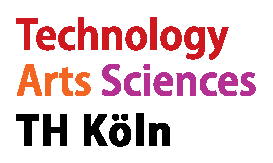
\includegraphics[scale=1.00]{img/logo_TH-Koeln_CMYK_22pt}\\
    \begin{center}
      \Large
      Technische Hochschule Köln\\
      Fakultät für Informatik und Ingenieurwissenschaften\\
      \hrule\par\rule{0pt}{2cm} % Horizontale Trennlinie  mit 2 cm Abtand nach unten erzeugen
      \LARGE
      \textsc{B A C H E L O R A R B E I T}\\
      \vspace{1cm} % Vertikaler Abstand von 1cm erzeugen
      \huge
      Entwicklung von Darstellungs- und Interaktionsmöglichkeiten in Virtual Reality für das Cranach Digital Archive\\
      \vspace{1cm}
      \large
      Vorgelegt an der TH Köln\\
      Campus Gummersbach\\
      im Studiengang\\
      Medieninformatik\\ 
      \vspace{1.0cm}
      ausgearbeitet von:\\
      \textsc{Nikolas Beckel}\\
      (Matrikelnummer: 11103435)\\
      \vspace{1.5cm}
      \begin{tabular}{ll} % Einfache Tabelle ohne Rahmen, mit 2 Spalten erzeugen
          \textbf{Erster Prüfer:} & Prof. Christian Noss \\
          \textbf{Zweiter Prüfer:} & Matthias Groß \\
      \end{tabular}
      \vspace{1.5cm}
      \\Gummersbach, im November 2020
    \end{center}    
  \end{titlepage}

  % Inhaltsverzeichnis
  \tableofcontents
  \newpage

  % Abbildungsverzeichnis
  \section*{Abbildungsverzeichnis}
  \addcontentsline{toc}{section}{Abbildungsverzeichnis} % Manuellen Eintrag im Inhaltsverzeichnis erzeugen
  \renewcommand{\listfigurename}{} % Name des Abbildungsverzeichnisses ändern
  \listoffigures

  % Tabellenverzeichnis
  \section*{Tabellenverzeichnis}
  \addcontentsline{toc}{section}{Tabellenverzeichnis} % Manuellen Eintrag im Inhaltsverzeichnis erzeugen
  \renewcommand{\listtablename}{} % Name des Abbildungsverzeichnisses ändern
  \listoftables
  \newpage

  \pagestyle{plain}

  % Die Bachelorarbeit
  \section{Einleitung}
    % \begin{itemize}
    %   \item Das Thema vorzustellen
    %   \item Das Ziel vorzustellen
    %   \item Den Leser neugierig machen
    %   \item Die Relevanz zu beschreiben
    % \end{itemize}
      
    Virtual Reality ist nicht mehr nur Zukunftsmusik oder ein Anwendungsbereich für Forscher
    großer Konzerne; immer mehr kommt Virtual Reality auf den Massenmarkt. Wo zu Beginn
    leistungsfähige Computer benötigt wurden, entstehen nun All-in-One VR-Brillen\footnote{Oculus Quest 2 - All-in-One VR-Brille | \url{https://www.oculus.com/quest-2/} (21.09.2020)}.
    Die Anwendungsbereiche von Virtual Reality sind vielfältig: Gaming, Unterhaltung durch VR-Filme oder
    das Treffen von Freunden in virtuellen Welten\footnote{Mozilla Hubs | \url{https://labs.mozilla.org/projects/hubs/} (21.09.2020)}.
    Die Pandemie durch das Virus SARS-CoV-2 hat uns auch gezeigt, dass immer mehr digitale Lösungen
    benötigt werden. Durch solche Krisen bekommen plötzlich Anwendungsbereiche, die nicht als
    notwendig betrachtet wurden, völlig neue Relevanz.
    Durch Virtual Reality ist man nicht mehr an einen Ort gebunden und kann gewisse Aktionen
    statt in der realen Welt, in einer virtuellen Welt ausführen. Von der realen Welt
    losgelöst, entstehen so auch völlig neue Möglichkeiten, diese aufzuführen.
    In dieser Bachelorarbeit wird das digitale Archiv der Cranachs\footnote{Cranach Digital Archive | \url{http://lucascranach.org/} (21.09.2020)}
    als Ressource genutzt, um neue Möglichkeiten der Darstellung für Kunst und Kultur zu erforschen.
    Dabei sollen aktuelle Entwicklungen, unter anderem aus dem musealen Bereich, miteinbezogen 
    und deren Erkenntnisse berücksichtigt werden.
    Auf Basis der recherchierten Ergebnisse sollen mehrere Prototypen entwickelt werden,
    die zeigen, wie Virtual Reality im Bereich Kunst und Kultur angewendet werden kann. 
    Dabei sollen die
    aktuellsten Technologien miteinbezogen und abgewägt werden, mit welcher die
    besten Ergebnisse erzielt werden können.

  \section{Grundlage und Datenbasis}
    In diesem Kapitel wird auf die Grundlagen von Virtual Reality, auf den Künstler Lucas Cranach 
    der Ältere und auf das Cranach Digital Archive eingegangen. Letzteres stellt 
    die Datenbasis für dieses Projekt dar, welches in der Entwicklung der Prototypen 
    eingesetzt wird. 
    Auf diesem Grundwissen baut das weitere Kapitel auf, welches genauer 
    die allgemeine Technologie von Virtual Reality thematisiert und weitergehend
    den musealen Anwendungsbereich miteinbezieht.

    \subsection{Das Cranach Digital Archive}
      Das Cranach Digital Archive ist eine Initative und ein visionäres Forschungsprojekt, 
      welches sich zum Ziel gesetzt hat, alle relevanten Informationen, Dokumente und 
      Werke der Cranachs in einer digitalen Datenbank der Forschung und Öffentlichkeit zur 
      Verfügung zu stellen.
      So konnten bisher über 1600 Gemälde und 14000 Abbildungen digitalisiert und auf der 
      Webseite \url{lucascranach.org} veröffentlich werden, welche frei über das
      Internet zugänglich ist.
      Bei den digitaliserten Aufnahmen der Werke handelt es sich nicht nur um hochauflösende
      Gemälde, sondern auch Röntgenaufnahmen, Infrarotreflektogramme und
      Archivalien. Dadurch lassen sich verschiedene
      Gemälde der Cranachs aus einer völlig neuen Perspektive betrachten, denn durch die
      Infrarotreflektogramme lassen sich zum Beispiel Unterzeichnungen
      eines Gemäldes erkennen, welches das bloße Auge niemals sehen könnte. [\cite{heydenreich2017lucas}]
    \subsubsection{Lucas Cranach der Ältere}
      Lucas Cranach d. Ä. war nicht nur ein erfolgreicher Künstler während der Renaissance,
      sondern auch ein guter Freund Martin Luthers. Gemeinsam ermöglichten sie eine moderne 
      Auffassung der Kunst.
      Lucas Cranach d. Ä. wurde 1472 als Sohn des Malers Hans Moller geboren,
      der ihn in der Zeichenkunst unterrichtete.
      Obwohl er früh mit dem Malen begonnen hatte, wurde Lucas Cranach d. Ä. erst in Wien
      um 1502 als Künstler bekannt. Um 1504/05
      verließ er Wien und nahm den Beruf des Hofmalers in Wittenberg für Friedrichs III. 
      entgegen, von welchem er auch sein zukünftig verwendetes Wappen verliehen bekommen 
      hatte.
      Dieses Wappen, eine \glqq geflügelte, bekrönte und einen Ring im Maul tragende
      Schlange\grqq{} [\cite[15]{heydenreich2017lucas}], sollte fortan als Signet von
      Lucas Cranach und seiner Werkstatt werden.
      Nach dem Tod von Friedrich III., diente er dessen Sohn und Nachfolger
      Johann I., welcher das Amt jedoch nur sieben Jahre lang führen konnte und
      schließlich an seinen Sohn, Johann Friedrich I. abgegeben hat.
      Bis zu seinem Tod stand Lucas Cranach d. Ä. im Dienst dieser drei Kurfürsten.
      Lucas Cranach d. Ä. zeichnete sich nicht nur durch die Qualität seiner Gemälde aus,
      sondern war auch dafür bekannt, produktiv zu arbeiten.
      Im Gegensatz zu seiner Konkurrenz malte er seine Gemälde nicht in freier
      Natur, sondern baute sich bereits in Wittenberg eine Werkstatt auf, die es
      ihm erlaubte, seine Produktivität auf eine neue Ebene zu bringen.
      Auch die Kunstgattung \glqq Druckgrafik\grqq{}, die Martin Luther 
      als Graben bezeichnete, erlaubte es
      Lucas Cranach d. Ä. einzelne Gemälde mehrfach zu drucken.
      Er war jedoch nicht nur als Künstler erfolgreich, sondern belegte in Wittenburg
      zwischen 1519 und 1544/45 das Amt des Ratsherren und einige Jahre davon auch als
      Kämmerer oder Bürgmeister.
      Die letzten Jahre von Lucas Cranach d. Ä. waren durch den Schmalkaldischen Krieg
      geprägt und beeinflusst, da Johann Friedrich I. mit seinen Truppen gegen den
      Kaiser kämpfte. Nach einer Niederlage und
      Verlusten seines Territoriums, foltge Lucas Cranach d. Ä. Johann Friedrich I.
      in die Gefangenschaft und verblieb dort von 1547 bis 1552.
      Nach der Gefangenschaft kehrte Lucas Cranach d. Ä. nach Weimar zurück und starb
      am 16. Oktober 1553 im Haus seiner Tochter.
      Zusammenfassend war Lucas Cranach d. Ä. nicht nur ein einfacher Künstler, sondern
      aufgrund seiner Qualität, Produktivität und humanistischem Denken
      seiner Zeit voraus. So legte er einen wichtigen Grundstein für die moderne
      Kunst. [\cite{heydenreich2017lucas}]
    \subsubsection{Martin Luther als Junker Jörg}
      Als Martin Luther 1511 nach Wittenburg zurückkehrte und 1512 die Professur für
      Bibelauslegung übernommen hatte, traf er zum ersten Mal auf Lucas Cranach d. Ä.
      Die beiden pflegten nicht nur engen Kontakt zueinander, sondern ergänzten sich auch
      in ihrer Arbeit. Martin Luthers Gedanken der Reformation konnten nicht nur in
      Schrift verbreitet werden, sondern auch durch das künstlerische Talent und die
      Produktivität von Lucas Cranach d. Ä. grafisch unterlegt werden. 
      Martin Luther nahm nachweislich die Dienste von 
      Lucas Cranach d. Ä. für Tiefenholzschnitte entgegen, welche auch für
      theologische Argumentationen benutzt wurden. Lucas Cranach d. Ä. trug auch
      dazu bei, dass es ein öffentliches Bild von Martin Luther gab und versuchte dieses
      zu manifestieren. Als 1521 die Reichsacht über Martin Luther verhängt wurde, 
      musste er aus Schutz seinen Tod durch einen inszenierten Überfall vortäuschen.
      Sein enger und guter Freund Lucas Cranach d. Ä. war jedoch über die Inszenierung 
      informiert. 
      Als Martin Luther zurück nach Wittenburg kehrte, um die dortigen Unruhen zu besänftigen, 
      trat er unter dem Pseudonym \glqq Junker Jörg\grqq{} auf. 
      Auch hier nahm Lucas Cranach d. Ä. eine entscheidende Rolle ein, da er in dieser 
      Zeit Bildnisse von Martin Luther anfertigte. 
      Beispielsweise wurde zu dieser Zeit ein Bildnisholzschnitt
      von Martin Luther als Junker Jörg gefertigt, welche absichtlich zur Medienstrategie
      verwendet wurde. So überbrachte Lucas Cranach d. Ä. die Nachricht, dass Martin Luther
      den inszenierten Überfall überlebte und vermittelte damit auch das Bild eines 
      entschlossenen und visionären Mannes. [\cite{heydenreich2017lucas}]
      \newline
      In diesem Forschungsprojekt wird sich auf die Datenbasis von Martin Luther als
      Junker Jörg des Cranach Digital Archive bezogen. Zur Entwicklung einer Antwort auf
      die Forschungsfrage wird nicht die gesamte Datenbasis des Cranach Digital Archive
      benötigt, da eine geringe Datenmenge zur Entwicklung von Virtual Reality-Szenen
      bereits ausreichen. Das Team hinter \url{lucascranach.org} hat die Daten bereits
      digitalisiert und aufgearbeitet, sodass Werke und Gemälde, die miteinander
      verwandt sind oder in Beziehung stehen, bereits zusammenhängend verknüpft sind.
    \subsection{Konzept und Nutzung von Virtual Reality} \label{Konzept und Nutzung von VR}
      Virtual Reality stammt aus dem Wissenschaftsgebiet der Computergrafik, denn eine
      virtuelle Realität besteht immer aus einer dreidimensionalen Simulation [\cite[13]{Dorner2013}].
      Es gibt mehrere Wege, eine virtuelle Realität zu simulieren. Nicht immer ist eine 
      VR-Brille notwendig, doch ist heutzutage das Nutzen solch einer Brille, um in eine 
      virtuelle Realität einzutauchen, state of the art. Das zeigt auch die schnelle 
      Entwicklung dieser Branche, die vermehrt auf VR-Brillen setzt, welche ohne einen
      zusätzlichen Computer auskommen. Die gesamte Echtzeitsimulation der virtuellen
      Realität wird innerhalb der VR-Brille berechnet\footnote{Oculus Quest 2 - All-in-One VR-Brille | \url{https://www.oculus.com/quest-2/} (21.09.2020)}.
      Sollte die Leistung der Brille nicht ausreichen, lassen sich diese optional mit einem
      Computer verbinden. Bei VR-Displays werden stereoskopische Verfahren angewandt [\cite[13]{Dorner2013}],
      wodurch Objekte, die durch die VR-Brille gesehen werden, einen Tiefeneffekt erhalten.
      Dieser Tiefeneffekt lässt virtuelle Objekte real erscheinen, da sie erstmals für unser
      Gehirn eine erkennbare räumliche Position aufweisen. Ein weiterer wichtiger
      Bestandteil von Virtual Reality ist die blickabhängige Bildgenerierung [\cite[13]{Dorner2013}].
      Bei der Bewegung des Kopfes, und damit des Blickpunktes des menschlichen Auges, wird
      die virtuelle Welt aus dem Blickwinkel, in welchen das
      menschliche Auge in der virtuellen Welt schaut, neu generiert. Da Virtual Reality 
      es erlaubt, Objekte
      aus verschiedenen Perspektiven zu sehen und auch mit diesen zu interagieren, gibt
      es vielfältige Einsatzmöglichkeiten. Das Virus SARS-CoV-2 hat gezeigt, dass es
      immer wichtiger wird von zu Hause aus arbeiten zu können oder Dienstleistungen von
      zu Hause aus entgegenzunehmen. Auch Museen oder Kunstgalerien können von
      Virtual Reality profitieren, da so die Kunst auf verschiedenen
      Wegen übermittelt werden kann. Die Darstellung ist nicht mehr an das klassische Bild 
      eines großen
      Raumes mit Gemälden an der Wand gebunden, sondern kann räumliche Limitierungen der
      realen Welt überwinden. Das Cranach Digital Archive ist eine große Datenbank mit
      vielen Gemälden und Archivalien. Einige Gemälde haben eine Beziehung zu anderen 
      Gemälden, da sie zum Beispiel zur selben Zeit entstanden sind, oder auf dem selben
      Bildträger angebracht wurden. Virtual Reality kann Forschern, aber auch 
      Kulturinteressierten, dabei helfen, die großen Datenmengen besser aufzunehmen und
      zu verstehen [\cite[9]{Dorner2013}]. Im nächsten Kapitel wird der aktuelle
      Forschungsstand von Virtual Reality erläutert und aufgezeigt wie dieser 
      aktuell für Museen eingesetzt werden kann.
      % Grundlagen von VR (Was ist VR überhaupt) und warum ist es im Kontext dieser BA wichtig? 
      % - Darstellung der Kunstwerke in 3D
  \section{Theoretische Einordnung}
    In diesem Kapitel wird das Thema Virtual Reality genauer behandelt, auf welchem
    Forschungsstand sich diese Branche befindet und welche Lösungen bereits auf 
    dem Markt sind. Mit Hilfe von Fachliteratur zu diesem Themenbereich sollen die
    aufgeworfenen Forschungsfragen beantwortet werden. Dieses Kapitel stellt das
    wissenschaftliche Fundament für die Entwicklung der Prototypen, die anhand der in
    diesem Kapitel gewonnenen Fakten entwickelt werden sollen. Zunächst wird der aktuelle
    Forschungsstand der VR-Branche betrachtet, welche technologischen
    Möglichkeiten und welche Produkte im musealen Bereich bereits existieren.
    Durch andere VR-Produkte, die ebenfalls im musealen Bereich entwickelt wurden, lassen
    sich Fehler vermeiden und etablierte Ideen für das eigene Produkt umsetzen.
    \subsection{Aktueller Forschungsstand von Virtual Reality}
      Virtual Reality ist mittlerweile eine Branche, welche Einzug in viele Bereiche der
      Industrie gefunden hat. Die Automobilindustrie nutzt Virtual Reality um Prototypen
      zu entwickeln. Durch dieses Vorgehen lassen sich Materialkosten sparen und auftretende
      Fehler frühzeitig erkennen. Die Medizin kann anhand von Virtual Reality die
      Ausbildung von angehenden Ärzten vereinfachen, da diese in einer virtuellen Welt
      den menschlichen Körper besser betrachten und dementsprechend verstehen können. Und
      die Spiele-Industrie, die einen großen Teil zur Entwicklung von
      VR-Brillen auf dem Massenmarkt beigetragen haben, erfährt ganz neue Möglichkeiten 
      den Spielern ein einzigartiges Spielerlebnis zu geben. Virtual Reality wird 
      in weiteren Branchen Anwendung finden und in naher Zukunft zu
      einer Technologie gehören, auf die sich nicht mehr verzichten lässt.
      \subsubsection{Entstehung}
        Virtual Reality ist keine neuartige Technologie, sondern existiert
        bereits seit den 60er Jahren. Ivan Sutherland forschte als Erster an immersiven 
        Technologien und führte so mit seinem Buch \glqq The Ultimate Display\grqq{} 
        den Rechner, das Design, die Konstruktion und Navigation virtueller Welten zusammen.
        In den 80er Jahren entwickelte die NASA erstmals mit dem Projekt VIEW (Virtual 
        Environment Interface Workstations) einen multisensorischen Arbeitsplatz, welcher für 
        die Simulation virtueller Weltraumstationen genutzt wurde.
        Der Begriff Virtual Reality wurde erstmals 1987 von einem Wissenschaftler namens Jaron
        Lanier verwendet. Er und Thomas Zimmermann gründeten gemeinsam die Firma VPL, welche
        am \glqq DataGlove\grqq{} arbeitete und diesen verkaufte. Dieser Handschuh konnte 
        mit Hilfe
        von Glasfasern Fingerdaten erfassen. Neben dem Handschuh verkauften sie auch das 
        \glqq EyePhone\grqq{}, eine Weiterentwicklung des Head-Mounted-Displays von Ivan
        Sutherland aus den 60ern.
        1989 wurde ein weiterer Meilenstein erreicht, denn die Firma Polhemus entwickelte 
        einen elektromagnetischen Tracker, welcher ein Ziel in bestimmter Entfernung vom 
        Rechner bestimmen konnte. 
        Zeitgleich entstand BOOM (Binocular Omni-Orientation Monitor) von Fake Space Labs.
        BOOM war ein 3D-Sichtgerät mit einem 1280x1024 Pixel Display, welches 1991 zum 
        ersten Mal Anwendung im \glqq Virtual Windtunnel\grqq{} von Steve Bryson fand, 
        einem Bereich der Luft- und Raumfahrt.
        1988 kamen mehr und verschieden hochwertige Arbeitsplätze für den Bereich Grafik 
        auf den Markt.
        Silicon Graphics konnte sich mit ihrer SGI Reality Engine 1995 weltweit durchsetzen
        und wurde so zum Standard dieser Branche. Damit kamen dann die ersten kommerziellen
        VR-Softwaresysteme auf den Markt.
        Die nächste große technologische Innovation wurde daraufhin vom Unternehmen SensAble
        Technologies Inc. vorgestellt, welches vom Massachusetts Institut of Technologies
        gegründet wurde. SensAble entwickelte ein haptisches Gerät namens 
        \glqq PHANtom\grqq{}, welches berührt werden musste, um eine
        Kraftrückkopplung spüren zu können.
        Anfang der 90er Jahre, nachdem schon einige technische Innovationen auf dem Markt
        erschienen sind, wurden viele wichtige Forschungen im Bereich der Virtual Reality
        unternommen, die sich vor allem auf Stereoleinwände konzentriert haben.
        Nach den Tracking-Systemen auf Basis von Elektromagnetismus folgten Systeme auf
        Basis von Ultraschall. Gegen 2000 wurde der Ultraschall jedoch von Infrarot
        abgelöst. Tracking-Systeme auf Basis von Infrafrot finden noch heute Anwendung im
        Bereich der modernen VR-Brillen.
        Die von Silicon Graphics entwickelte SGI Reality Engine, welche in vielen
        VR-Softwaresystemen verwendet wurde, wurde langfristig auch von Computern
        abgelöst. Die damit einhergehende Preissenkung (circa um $\frac{1}{5}$)
        erlaubte umfangreichere Forschungen.
        Historisch betrachtet hat auch Deutschland einige Unternehmen vorzuweisen, die sich
        bereits seit 1998 mit VR-Systemen beschäftigen. So sind beispielsweise VRCOM, 
        RTT und IC:IDO zu nennen.
        Ein ständiger Austausch zum Wissenschaftsgebiet Virtual Reality fand demnach international
        und auf Länderebene statt. Schließlich konnte sich die IEEE VR Konferenz
        international durchsetzen und ist jährlich mit etwa 500 Teilnehmern einer der
        größten Konferenzen zu diesem Thema.
        Seit 2003 hat zudem die Gesellschaft für Informatik eine Fachgruppe für das Thema
        Virtual und Augmented Reality. [\cite[19-21]{Dorner2013}] \\
        Heutzutage haben sich die Head-Mounted-Displays, oder einfach VR-Brillen genannt,
        mit Infrarot als Sensorik auf dem Massenmarkt durchgesetzt. Diese sind sehr kompakt
        und benötigen, je nach Anbieter, keinen Computer mehr. Sie funktionieren autark und
        übernehmen jegliche Berechnung in der VR-Brille. Vorreiter dieser Branche sind unter
        anderem Oculus von Facebook und Vive von HTC in Kooperation mit Valve.
      \subsubsection{Wahrnehmungsaspekte} \label{Wahrnehmungsaspekte}
        Wie Menschen Informationen wahrnehmen, ist ein wichtiger Aspekt für die Gestaltung
        von virtuellen Welten. In einer perfekten virtuellen Realität würde der Konsument
        alle Sinneseindrücke, die er aus der realen Welt kennt, in der simulierten Welt
        in gleicher Qualität und Quantität empfinden können [\cite[17]{Dorner2013}].
        Doch so eine perfekte virtuelle Realität zu entwickeln ist nach aktuellem Stand
        der Technik nicht möglich. Die heutigen VR-Systeme und -Technologien
        konzentrieren und beziehen sich auf den visuellen, akustischen und haptischen Sinn
        des Menschen [\cite[34]{Dorner2013}]. Dementsprechend nutzt ein ideales
        VR-System jene Effekte in Kombination mit einem
        Tracking-System [\cite{Slater2009}]. Die heutige Technologie ist bereits auf
        dem Stand, dass alle drei genannten Sinne angesprochen und beeinflusst
        werden können. Die VR-Brillen selbst besitzen ein Tracking-System für das
        Bewegen des Kopfes sowie die Veränderung der räumlichen Position und mehrere 
        3D-Eingabegeräte,
        die das Bewegen der Hände analysieren können. Die Immersion einer VR-Erfahrung
        wird auch nicht zwingend durch die Bildschirme und das Tracking-System bestimmt,
        sondern durch die Anzahl der ausführbaren Aktionen innerhalb der virtuellen 
        Welt [\cite{Slater2009}]. So hilft der technologische Fortschritt der 
        heutigen VR-Brillen
        sehr bei der Entwicklung von virtuellen Welten, jedoch müssen auch die
        durchführbaren Aktionen gut umgesetzt sein. Denn einer der wichtigsten Aspekte
        für das Wahrnehmen von virtuellen Welten ist das Gefühl der 
        Präsenz [\cite{Slater2009}]. \\
        Die Präsenz beschreibt das Gefühl, in der 
        virtuellen Welt zu sein [\cite{Slater2009}]. 
        Dabei weiß der Benutzer jedoch zu jedem Zeitpunkt, dass er
        nicht wirklich dort ist [\cite{Slater2009}]. Grundlegend lässt sich der 
        Aspekt der Präsenz in
        drei Unteraspekte aufteilen: Das Gefühl der Ortsillusion, die Plausibilitätsillusion
        und die Involviertheit [\cite[18-19]{Dorner2013}]. Eine virtuelle Welt sollte immer unter
        Berücksichtigung dieser drei Gefühle entwickelt werden, da eine gute Umsetzung
        dieser die beste Nutzungserfahrung für einen Benutzer sicherstellen kann. \\
        Bei der 
        Ortsillusion handelt es sich um die starke Illusion an einem Ort zu sein, mit dem
        Wissen, dass man nicht wirklich dort ist [\cite{Slater2009}]. Einer der wichtigsten
        Kriterien, um diese Illusion beim Benutzer zu erreichen, ist die in Kapitel 
        \ref{Konzept und Nutzung von VR}
        erwähnte blickpunktabhängige Bildgenerierung der VR-Brille [\cite[18]{Dorner2013}]. \\
        Bei der Plausibilitätsillusion handelt
        es sich um das Gefühl, dass die Geschehnisse innerhalb der virtuellen Welt 
        wirklich passieren, mit dem Wissen, dass dies nicht wirklich passiert
        [\cite{Slater2009}]. Eine Schlüsselkomponente, um diese Illusion hervorzurufen,
        sind Geschehnisse, die nicht vom Benutzer ausgelöst wurden, sich jedoch auf ihn
        beziehen [\cite{Slater2009}]. Das können beispielsweise auf den Benutzer zufliegende
        Projektile sein oder ein virtueller Mensch, der den Benutzer anspricht
        [\cite[18-19]{Dorner2013}]. Die Geschehnisse die innerhalb der virtuellen Realität
        stattfinden müssen jedoch nicht physikalisch realistisch sein [\cite{Slater2009}]
        und können dementsprechend auch fantasievoll und unrealistisch sein. Als Beispiel kann
        ein Spiel genommen werden, in welchem der Benutzer von einem Magier mit einem 
        Feuerball angeschossen wird; der Benutzer hat das Ereignis nicht selber ausgelöst,
        wird jedoch in das Geschehen eingebunden. Eine Plausibilitätsillusion entsteht,
        obwohl das Szenario unrealistisch ist. So kann diese durch das
        Einbauen von realistischen Effekten, wie Schatten oder die Darstellung des eigenen
        Körpers, verstärkt werden [\cite{Slater2009}]. \\
        Das Anzeigen des Körpers des Benutzers
        kann sogar den Effekt der Orts- und Plausibilitätsillusion verstärken, da das
        Gefühl in der virtuellen Realität zu sein realer erscheint und 
        dementsprechend auch Geschehnisse die den
        Benutzer betreffen [\cite{Slater2009}]. Genauso können beide Illusionen durch das
        Ausnutzen der Ängste eines Menschen hervorgerufen werden [\cite{Slater2009}].
        Leidet der Benutzer unter Höhenangst, dann wird er ebenfalls in der virtuellen
        Welt unter Höhenangst leiden, wenn er sich beispielsweise auf einem Hochaus 
        befindet und die Kante herunterschaut. 
        Demnach verstärkt sich das Gefühl, dass die virtuelle Realität Wirklichkeit sei,
        obwohl der Benutzer zu jedem Zeitpunkt weiß, dass es sich um eine Simulation handelt.
        So kann einer immersiven
        virtuellen Realität gesprochen werden, wenn der Benutzer so handelt und agiert, wie er es
        in einer realen Welt tun würde (\glqq Response-as-if-real\grqq{} (RAIR)) 
        [\cite{Slater2009}]. Diese genannten Aspekte (Immersion, Ortsillusion, 
        Plausibilitätsillusion und das Darstellen des eigenen Körpers) stellen ein 
        Framework dar, wonach virtuelle Realitäten entwickelt werden können 
        [\cite{Slater2009}]. Diese Aspekte stellen auch Gefühle dar, welche der Benutzer
        während seiner Erfahrung empfinden kann und die es gilt gut umzusetzen.
        Fehlerhafte Darstellungen können die Ortsillusion negativ beeinflussen.
        Darüber hinaus ist es durch das Beheben der Fehler jedoch möglich, jene Illusion
        wiederherzustellen [\cite{Slater2009}].
        Anders verhält sich die Plausibilitätsillusion, welche schwer
        zu erreichen ist. Sofern diese einmal gebrochen ist, kann sie in der aktuellen 
        Erfahrung des Benutzers nicht mehr oder nur schwer wieder aufgenommen werden 
        [\cite{Slater2009}].
        Ein Beispiel für den Bruch der Plausibilitätsillusion ist ein virtueller Mensch,
        mit dem kommuniziert werden kann, er aber nur in sehr einfachen Phrasen antwortet
        [\cite[19]{Dorner2013}]. So geht die Glaubwürdigkeit der Illusion verloren. 
        Deshalb 
        sollten virtuelle Realitäten so wenig Raum für Fehler bieten wie nur 
        möglich [\cite{Slater2009}]. \\
        Die Involviertheit ist neben der Orts- und Plausibilitätsillusion ein weiteres
        Gefühl, welches die Qualität der Nutzungserfahrung steigert. Sie
        beschreibt das Verhältnis der Aufmerksamkeit und des Interesses eines Benutzers zur
        virtuellen Realität [\cite[227]{Witmer1998}]. Je höher die Aufmerksamkeit und das
        Interesse des Benutzers, desto höher ist die Qualität der Nutzungserfahrung.
        Geräusche aus der realen Umgebung, oder das unbequeme Sitzen der VR-Brille, können
        bereits die Aufmerksamkeit und das Interesse stark senken und somit die Qualität
        der Erfahrung beeinträchtigen [\cite[227]{Witmer1998}].
        Abgesehen der drei oben genannten Aspekte, lässt sich die Nutzungserfahrung durch
        Berücksichtigung technischer Aspekte verbessern. Darunter fällt die
        Bildwiederholungsrate der Anwendung, die Bildschirmauflösung, das Gesamtausmaß und
        die Latenz des Trackings, der Grad des Sichtfelds und die visuelle Qualität der Umgebung
        und ihrer Objekte [\cite{Slater2009}].
        Unter Berücksichtigung dieser Gesichtspunkte können qualitativ hochwertige
        virtuelle Realitäten entwickelt werden, welche durch das Ansprechen 
        der richtigen Gefühle des Benutzers eine erfolgreiche 
        Nutzungserfahrung hervorbringen können.
      \subsubsection{VR-Brillen}
        Neben den gesamten Aspekten, die es für die Erstellung von
        Nutzungserfahrungen innerhalb virtueller Welten zu berücksichtigen gibt, 
        muss das technische System ebenfalls jene Aspekte
        abbilden können. In der heutigen Zeit haben sich VR-Brillen 
        (auch Head-Mounted-Displays genannt) in 
        Kombination mit 3D-Eingabegeräten durchgesetzt. Diese sind mittlerweile sehr kompakt,
        leistungsstark und preislich erschwinglich. Dadurch, dass Hardware kleiner
        und günstiger wird, kann der Trend beobachtet werden, dass VR-Brillen auch ohne
        einen stationären Computer funktionieren.
        Den Vorteil von VR-Brillen, im Gegensatz zu Projektionssystemen, bildet die 
        Möglichkeit, diese überall anziehen und nutzen zu können [\cite[129]{Dorner2013}].
        Dementsprechend haben sich Head-Mounted-Displays als VR-Systeme auf dem Massenmarkt
        durchgesetzt, da diese kompakt sind und nicht zwingend einen Computer benötigen.
        Zudem ist je nach Anwendungsfall eine VR-Brille nicht notwendig, da heutige 
        mobile Endgeräte, wie Smartphones, bereits genügend Leistung für eine 
        Echtzeit-Simulation mitbringen. So gibt es Aufsätze für das Smartphone,
        mit welchen es sich in eine VR-Brille umfunktionieren lässt (siehe Abb. \ref{fig:google-cardboard}\footnote{Google Cardboard | \url{https://arvr.google.com/cardboard/} (18.10.2020)}).
        Da diese Lösung kostengünstig und einfach umzusetzen ist, gilt dies als 
        gute Einstiegsmöglichkeit für Personen, die gerne
        VR-Erfahrungen erleben würden, sich jedoch nicht eine autarke VR-Brille leisten
        möchten.
        \begin{figure}[t]
          \centering
          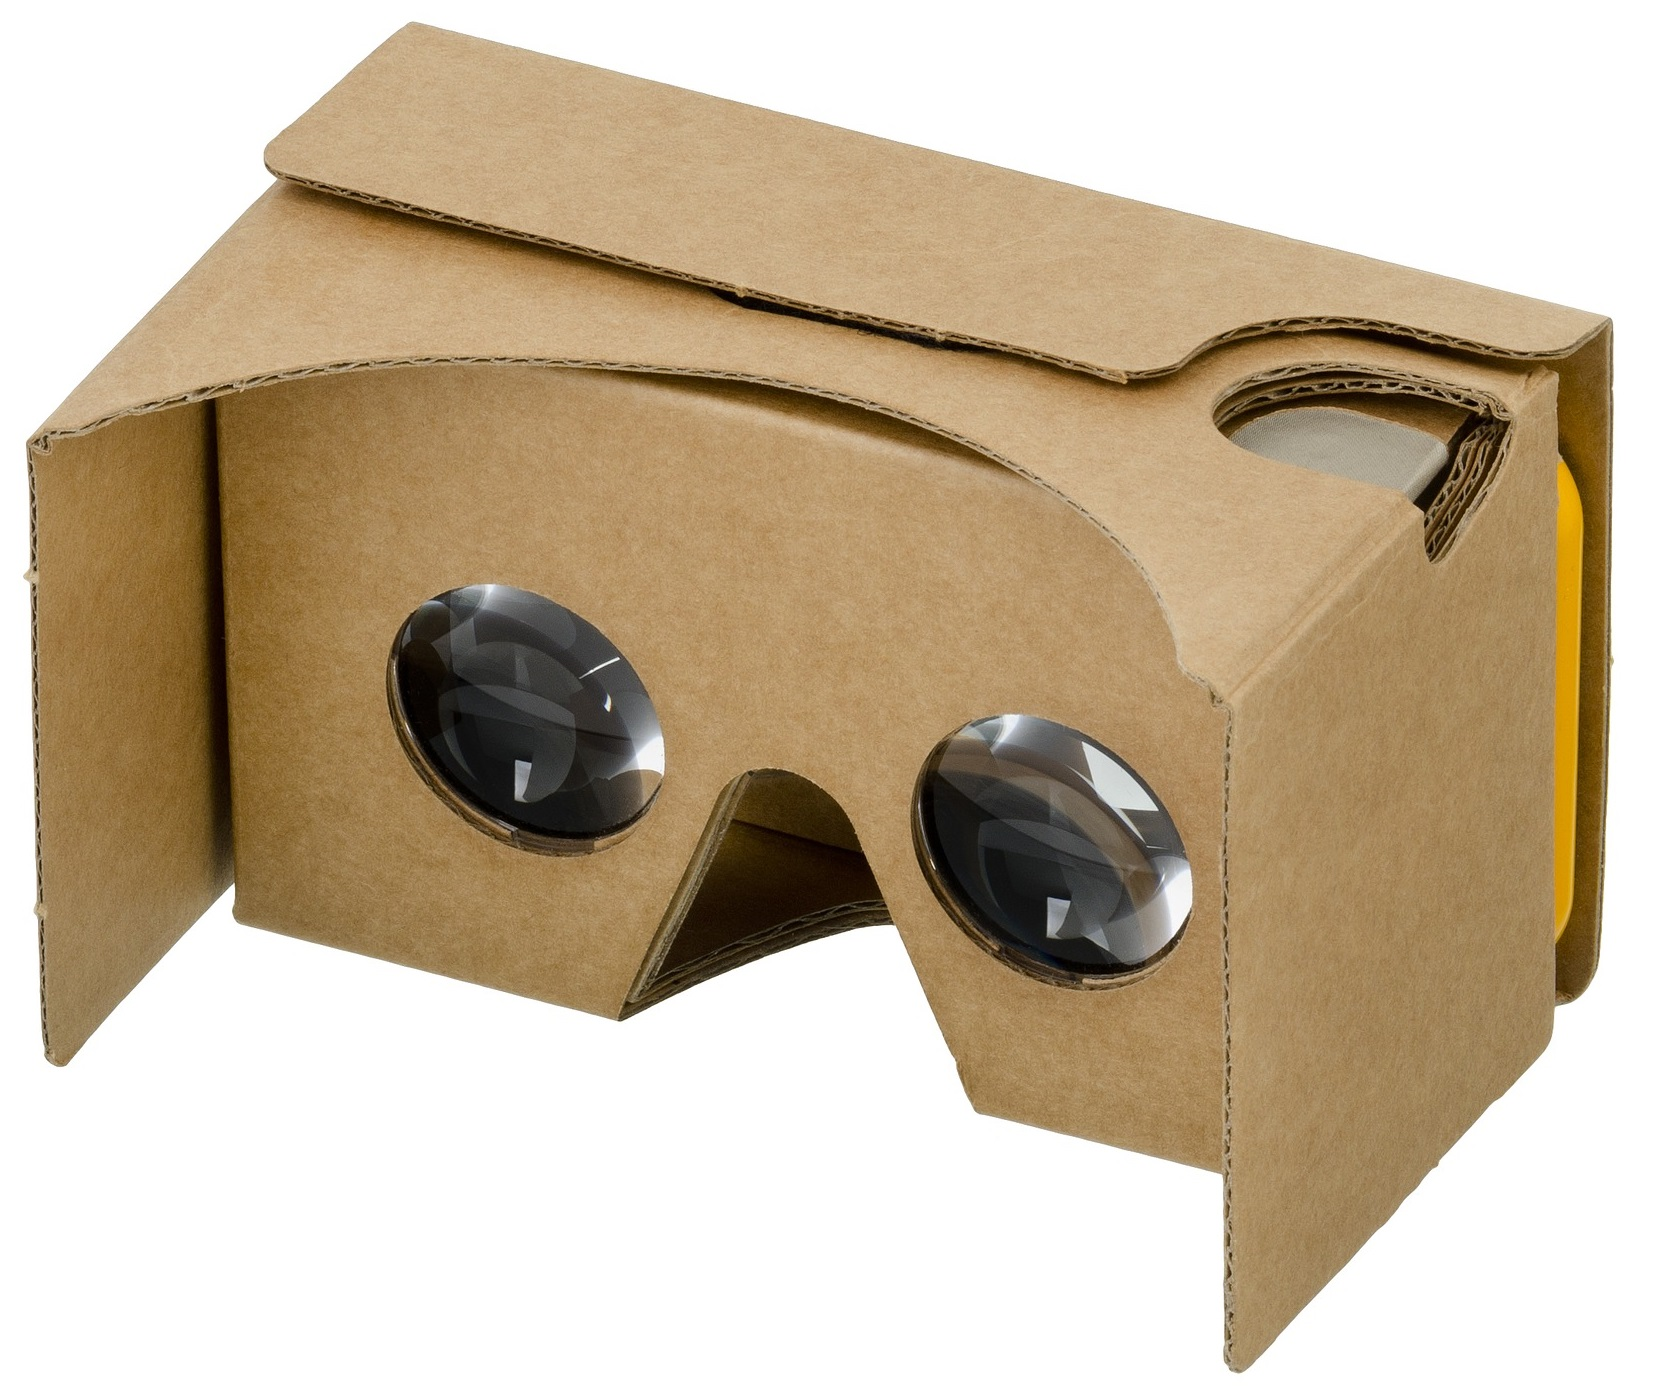
\includegraphics{img/google-cardboard.jpg}
          \caption{Google Cardboard für Smartphones.}
          \label{fig:google-cardboard}
        \end{figure}
        Doch ist durch das Fehlen der 3D-Eingaberäte bei dieser Lösung, je
        nach Anwendungsfall, eine Einschränkung festzustellen. Abhängig vom dem 
        jeweiligen Smartphone kann 
        auch eine geringe
        Bildschirmauflösung die in Kapitel \ref{Wahrnehmungsaspekte} genannten Aspekte
        beinträchtigen und einen Bruch der Illusionen hervorrufen.
        Projektionssysteme, die die simulierte Umgebung auf ganzen Leinwänden darstellen,
        haben den Vorteil, dass sich der Benutzer nicht unmittelbar vor dem Bildschirm
        befindet [\cite[134]{Dorner2013}]. Dadurch können keine einzelnen Pixel mit dem Auge 
        erfasst werden. Daraus ergibt sich, dass die Bildschirmauflösung ein wichtiges
        Kritierium zur guten Anwendung von VR-Brillen ist [\cite[134]{Dorner2013}].
        Aktuelle Unternehmen, die sich mit VR-Brillen beschäftigen und diese Technologie
        maßgeblich vorgeben, sind unter anderem Facebook mit Oculus
        \footnote{Oculus | \url{https://www.oculus.com/?locale=de_DE} (18.10.2020)}, 
        HTC mit Vive \footnote{HTC VIVE | \url{https://www.vive.com/de/} (18.10.2020)},
        Playstation mit PlaystationVR
        \footnote{PlaystationVR | \url{https://www.playstation.com/de-de/explore/playstation-vr/} (18.10.2020)}
        und Valve Corporation mit der Valve Index
        \footnote{Valve Index | \url{https://www.valvesoftware.com/de/index/headset} (19.10.2020)}.
        Samsung beschäftigt sich ebenfalls mit Virtual
        Reality, jedoch bieten diese nur eine hochwertige Brille ohne Rechenleistung an.
        Für den vollständigen Funktionsumfang wird zusätzlich ein Samsung Smartphone vorausgesetzt
        \footnote{Samsung Gear VR | \url{https://www.samsung.com/de/wearables/gear-vr-r323/} (18.10.2020)}.
        Auch Nintendo hat mit der Konsole Nintendo Switch den Weg zu Virtual Reality
        gefunden
        \footnote{Nintendo Labo VR-SET | \url{https://www.nintendo.de/Nintendo-Labo/Nintendo-Labo-1328637.html} (18.10.2020)}.
        Das VR-Set für die Nintendo Switch bietet sich hilfreich für Kinder an, um erste 
        Erfahrungen mit Virtual Reality machen zu können.
        Auch Google ist mit dem Google Cardboard in diesen Markt involviert, bietet jedoch keine 
        VR-Brille mit integrierter Hardware an.
      \subsubsection{Native und webbasierte Anwendungen}
        Viele VR-Brillen bedeuten auch viele Software-Development-Kits (SDK) die damit einhergehen. 
        VR-Anwendungen können heutzutage mit Hilfe von vielen Programmen oder Frameworks entwickelt
        werden. So kann ein Produkt nativ für eine Plattform entwickelt werden oder durch
        webbasierte Anwendungen plattformunabhängig funktionieren.
        Beide Ansätze bieten ihre Vor- sowie Nachteile und sind daher vom jeweiligen 
        Anwendungsfall abhängig.
        Native Lösungen bieten in der Softwareentwicklung eine geeignetere
        Performance, da diese Anwendungen mit Programmiersprachen entwickelt werden die
        effizient und maschinennah sind. Je nach Hersteller gibt es auch für das 
        Betriebssystem eigene Programmiersprachen, die dann für das jeweilige Ökosystem 
        optimiert werden können.
        Webanwendungen, die in der Regel auf Basis von JavaScript laufen, werden nicht 
        kompiliert sondern interpretiert und der Quellcode wird zur Laufzeit vom Browser 
        gelesen und ausgeführt.
        Durch eine große und aktive Community hat sich JavaScript in den letzten Jahren 
        zu einer universellen Programmiersprache entwickelt und findet Anwendung in
        fast allen Gebieten der Softwareentwicklung.
        Diese Entwicklung der letzten Jahre hat gezeigt, dass der Mensch weniger
        Zeit vor dem PC im Internet verbringt, sondern hauptsächlich mobil darauf zugreift 
        [\cite[1]{Ater2017}].
        Durch das Betrachten von Internetseiten auf einem mobilen Endgerät wurde der
        Ansatz mobile-first immer wichtiger [\cite[1]{Ater2017}]. Die Vorteile, die native
        Anwendungen mehrere Jahre mit sich brachten, waren, neben der besseren Leistung,
        erweiterte Grafikmöglichkeiten, Standortermittlung, Push-Benachrichtigungen,
        Offlineverfügbarkeit und Startbildschirm-Verknüpfungen [\cite[3]{Ater2017}]. Diese
        Funktionen waren damals notwendig für erfolgreiche Apps, da diese dem
        Benutzer eine bessere Nutzungserfahrung ermöglichten. 
        Heutzutage hat sich das Web als Plattform weiterentwickelt, sodass jene Funktionen nicht
        mehr nur nativen Anwendungen vorenthalten sind.
        Sogenannte Progressive Web Apps erlauben sich an nativen Funktionen der Plattform zu
        bedienen, bieten jedoch weiterhin die Flexibilität, die das Web mit sich bringt
        [\cite[2]{Ater2017}].
        So können webbasierte Anwendungen offlinefähig gestaltet werden. Darüber hinaus können
        Push-Benachrichtigungen von Webseiten verschickt werden und zudem lassen sich
        Desktop- und Startbildschirmverknüpfungen über moderne Browser anlegen [\cite[5-6]{Ater2017}].
        Durch das Ausblenden der URL-Leiste des Browsers
        undd as Ausführen der webbasierten Anwendung im Vollbildmodus, ähneln sich den
        native Anwendungen [\cite[6]{Ater2017}]. Für das Ziel einer Anwendung, diese
        möglichst zugänglich zu machen, ist die Entwicklung einer webbasierten Lösung
        vorteilhaft, da plattformunabhängig entwickelt werden kann und der
        Benutzer direkt am Ziel ist, sobald dieser die Webseite öffnet.
        Es muss kein zusätzlicher
        Download oder eine zusätzliche Installation erfolgen und auch das Pflegen mehrerer
        Versionen in den verschiedenen App Stores entfällt. So kann der Benutzer unabhängig
        seiner Plattform und seinem Gerät die Anwendung benutzen. Da der Benutzer 
        demnach an keine Plattform
        gebunden ist, ist die Möglichkeit höher, ein vielfaches mehr an potenziellen
        Benutzern zählen zu können [\cite[3]{Ater2017}].
        Es ist zunehmend schwieriger geworden Benutzer für den Download einer App 
        zu motivieren [\cite[3]{Ater2017}].
        Die meisten Benutzer gehen bereits auf dem Weg zum jeweiligen Store und der darauffolgenden
        Installation verloren [\cite[4]{Ater2017}]. Application Programming Interfaces (API) 
        wie die Web Share und Web Share Target
        API sind nur ein Teil der zukünftigen Entwicklung, die immer mehr Funktionen ins
        Web bringen, welche zuvor nur für native Anwendungen zur Verfügung standen [\cite[245]{Ater2017}].
        So findet auch Virtual Reality, durch die WebXR-Schnittstelle (ehemals WebVR),
        Anwendung im Browser [\cite[245]{Ater2017}]. In Kombination mit WebGL lassen sich komplexe,
        rechenintensive und überzeugende VR-Erfahrungen entwickeln [\cite[245]{Ater2017}].
        Die Schnittstelle WebXR ist kompatibel mit den gängigsten VR-Brillen und kann auch
        ihre jeweiligen 3D-Eingabegeräte lesen, wodurch der Entwickler Zugang zu allen Informationen
        bekommt, die auch eine native Desktop-Anwendung mitbringen würde [\cite[245]{Ater2017}].
        Im Punkt Leistung sind nach wie vor native Anwendungen einige Schritte voraus, doch
        gibt es jetzt schon bereits Lösungen, die an diesem Problem arbeiten. WebAssembly\footnote{Offizielle WebAssembly Webseite | \url{https://webassembly.org/} (02.11.2020)}
        ist eine niedere Programmiersprache, welche wenig Abstraktion zur Befehlssatzarchitektur
        des Computers bietet [\cite[185]{Haas2017Jun}]. Dadurch, dass WebAssembly zu ByteCode
        kompiliert wird, kann nahezu die native Leistung mit einer webbasierten Anwendung 
        erreicht werden
        [\cite[186]{Haas2017Jun}]. So bleibt weiterhin die Plattformunabhängigkeit geboten,
        da WebAssembly über den Browser ausgeführt werden kann.
        Jedoch ist WebAssembly noch nicht
        so verbreitet wie JavaScript und bietet deshalb weniger Technologien und Möglichkeiten,
        zur Entwicklung von VR-Anwendungen. Zum aktuellen Zeitpunkt bietet die Unity Engine
        die Möglichkeit, VR-Anwendungen mit Hilfe ihrer Engine zu entwickeln und
        diese für moderne Browser zu exportieren\footnote{WebAssembly in Unity | \url{https://blogs.unity3d.com/2018/08/15/webassembly-is-here/} (02.11.2020)}.
        Die Unreal Engine kompiliert den geschriebenen Code ebenfalls zu WebAssembly,
        hat die HTML5-Entwicklung jedoch als Erweiterung ausgelagert, die durch
        die Community weiterentwickelt werden soll\footnote{Unreal Engine Dokumentation für HTML5 Development | \url{https://docs.unrealengine.com/en-US/Platforms/HTML5/index.html} (02.11.2020)}.
        Da es in der klassischen Softwareentwicklung nicht sinnvoll ist in Assemblersprache
        zu entwickeln, macht es ebenfalls wenig Sinn selbstständig eine VR-Anwendung in 
        WebAssembly zu entwickeln. Deshalb wird eine höhere Programmiersprache benötigt, die
        eine höhere Abstraktion bietet. So ist es am einfachsten Unity oder Unreal Engine 
        als Software zu nutzen,
        um VR-Anwendungen auf Basis von WebAssembly zu generieren.
        Nach wie vor ist die Entscheidung, ob nativ oder für das Web entwickelt werden soll, 
        abhängig vom Anwendungsfall. 
        Für das Cranach Digital Archive bietet sich eine webbasierte Lösung
        an, da die Darstellung von Gemälden und Archivalien keine hochkomplexen Berechnungen
        benötigt. Das aktuelle Archiv ist über das Internet zu erreichen und lässt sich auf
        Desktop-PCs und mobilen Endgeräten betrachten. Das Archiv ist bereits über die größte
        Plattform aufzurufen, dementsprechend sollte die VR-Lösung ebenfalls
        über das Web zugänglich sein. So können auch Kunstinteressierte, die sich keine hochwertige
        VR-Brille leisten möchten, die Gemälde und Archivalien mit ihrem Smartphone erkunden.
        Durch eine plattformunabhängige Lösung ist weniger Wartung notwendig und das
        Bereitstellen in die jeweiligen App Stores entfällt, sodass viel Zeit und
        Ressourcen gespart werden können [\cite[248]{Ater2017}]. Webbasierte Anwendungen 
        benötigen die wenigsten Ressourcen für eine hohe Zugänglichkeit, wodurch sich dieser
        Entwicklungsansatz auch für das Forschungsprojekt anbietet, da die vorhandenen 
        Ressourcen gering sind.
    \subsection{Virtual Reality im musealen Kontext}
      Die Idee Kunst in einer virtuellen Realität darzustellen, ist keine neue Idee.
      Immer wieder wagten sich Museem daran, stellten Konzepte auf, sammelten
      Erfahrungsberichte und entwickelten eigene Produkte [\cite{Heidsiek2019}]. Es ist
      ein wichtiger und verständlicher Schritt, dass Virtual Reality
      im musealen Bereich vermehrt und umfangreich Anwendung findet. Museen versuchen Gefühle,
      Erfahrungen sowie Emotionen zu übermitteln und durch den Einsatz von Virtual Reality
      besteht die Möglichkeit, den Besucher in Szenarien zu versetzen, die in der
      Vergangenheit geschehen sind. Der Besucher kann auch Fantasiewelten der Künstler
      wahrnehmen, um ein besseres Verständnis für ihre Kunst zu erlangen. Umfragen ergaben, 
      dass ein generelles Interesse an neuartigen Technologien im Museum vorhanden ist [\cite[34]{Heidsiek2019}].
      Die Besucher erhoffen sich dadurch, dass Museen unterhaltsamer, lehrreicher und
      zugänglicher werden [\cite[34]{Heidsiek2019}]. Gerade Virtual Reality lässt Museen
      und Informationen für die breite Masse zugänglicher werden, denn die Besucher 
      sind nicht mehr gezwungen 
      das Museum physisch zu besuchen. Der Anwendungsbereich ist vielfältig und die 
      Technologie noch nicht ausgereizt.
      Doch birgen neue Technologien neben ihren Chancen auch Risiken, die berücksichtigt
      und disktutiert werden müssen. Deshalb wird in diesem Kapitel auf die
      Risiken und auch auf die Chancen eingegangen, die ein Museum bei einem Einsatz von
      Virtual Reality erwarten kann. Da das Cranach Digital Archive nicht das erste Museum ist, 
      welches Kunst digitalisiert, sollen bereits entwickelte Produkte analysiert
      werden, deren Erkentnisse und Ideen dabei helfen, bereits begangene Fehler zu 
      vermeiden und geeignete Prototypen zu entwickeln.
      \subsubsection{Chancen und Risiken}
        Museen sind Stätten des Wissens. Ihre Aufgabe besteht darin, Menschen Wissen zu
        vermitteln. Meist über vergangene Erfahrungen oder Geschehnisse. Durch die
        Digitalisierung und das Internet war es erstmals möglich, historische Gegenstände
        oder Gemälde mit der ganzen Welt zu teilen, unabhängig des Standortes eines
        Betrachters. Dementsprechend liegt der Mehrwert von digitalen Museen darin, eine
        erhöhte Vervielfältigung und Verbreitung von Wissen zu betreiben [\cite[17]{Huennekens2002}].
        Auch das Anwendunsgebiet Virtual Reality bietet nach dem Internet und der Digitalisierung
        eine neue Möglichkeit Informationen innovativ zu übermitteln [\cite[52]{Heidsiek2019}].
        So wird das Museum als Stätte des Wissens effizienter gestaltet und ermöglicht 
        mehr Menschen
        zu erreichen, als es vorher möglich war. Das Cranach Digital Archive geht hier mit
        gutem Beispiel voran und bietet eine umfangreiche Datenbank
        zu den Werken und Archivalien der Cranachs.
        Im Vergleich zu statischen Objekten, wie hängende Gemälde an Wänden, lassen sich 
        durch digitale Lösungen verschiedene und neue Darstellungen ermöglichen [\cite[17]{Huennekens2002}].
        Gerade Virtual Reality bietet hier eine sehr interessante Möglichkeit, völlig neue
        Perspektiven zu erschaffen, die niemals in der realen Welt erreicht werden können.
        Ein Vorteil in Virtual Reality liegt darin, dass die Gesetze von Raum und Zeit nicht
        in einer virtuellen Realität gelten [\cite[140]{Huennekens2002}]. So kann der Mensch
        seiner Begierde, alltägliche Erfahrungen zu überschreiten, nachkommen [\cite[140]{Huennekens2002}].
        Diese unendlichen Möglichkeiten bringen jedoch auch eine ethische 
        Verantwortung zur Präsentation musealer Gegenstände mit sich.
        Das Loslösen von Raum und Zeit kann sich negativ auf die historischen Inhalte auswirken
        [\cite[141]{Huennekens2002}]. So könnte sogar von Entweihung der historischen
        Gegenstände gesprochen werden [\cite[141]{Huennekens2002}]. Deshalb liegt es in der 
        Verantwortung der
        Museen die historische Integrität eines Gegenstandes oder einer Erfahrung nicht
        zu verletzen [\cite[38]{Heidsiek2019}]. Dies kann vermieden werden, indem 
        kenntlich gemacht wird, was original ist und was selbstständig hinzugefügt
        wurde [\cite[38]{Heidsiek2019}]. Sobald virtuelle Realitäten erfundene Aspekte 
        beinhalten, und diese nicht als solche gekennzeichnet wurden, handelt es sich nicht
        mehr um eine historische Überlieferung, sondern um persönliche und subjektive 
        Wahrnehmungen [\cite[38]{Heidsiek2019}]. Fotorealistische Darstellungen
        von unwahren Ereignissen oder Objekten können verstärkt dazu führen, dass der
        Benutzer von der fälschlichen Tatsache überzeugt wird [\cite[39]{Heidsiek2019}].
        So hat jedes Museum, dass Virtual Reality als Möglichkeit zur Betrachtung 
        kunstrelevanter Objekte anbieten möchte, die ethische Verantwortung, 
        dem Benutzer zu jedem Zeitpunkt kenntlich zu machen,
        was eine historische Übermittlung und was virtuelle Realität ist.
        Zudem besteht durch Virtual Reality die Gefahr, dass Museen, auf lange Sicht 
        betrachtet, obsolet werden und alles über eine VR-Brille erforscht werden kann
        [\cite[142-143]{Huennekens2002}]. Besucher die Virtual Reality in Museen genutzt
        haben, betrachten diese Technologie jedoch als Ergänzung zum Museum und nicht als
        einen vollständigen Ersatz, da der Hauptgrund eines Museumsbesuchs die Betrachtung
        der Originalobjekte sei [\cite[79]{Heidsiek2019}]. Originale Ausstellungsstücke
        haben demnach weiterhin einen nicht reproduzierbaren Charakter, welcher sich nicht 
        in einer
        virtuellen Realität darstellen lässt [\cite[93]{Heidsiek2019}]. So schwächt die
        Darstellungen von Originalobjekten als Kopie in einer virtuellen Welt
        die Authentizität dieser [\cite[93]{Heidsiek2019}]. 
        Besucher, die vorher eine Online-Ausstellung eines Museums gesehen haben,
        entschieden sich sogar aufgrund dessen für das Besuchen des Museums in der 
        realen Welt [\cite[777-778]{Katz2015}]. So kann eine VR-Erfahrung, die über
        das Web zu erreichen ist, nicht als Ersatz für das Museum gesehen werden,
        sondern auch als innovatives und modernes Marketingwerkzeug.
        Dementsprechend ist nach aktuellem
        Stand nicht davon auszugehen, dass die Technologie Virtual Reality das Museum in
        naher oder mittlerer Zukunft obsolet macht.
        Die Museumslandschaft sieht in Virtual Reality die Chancen, neue und andere
        Geschichten zu vermitteln, langfristig für Besucher attraktiv zu bleiben und
        auch eine neue Zielgruppe zu erreichen [\cite[34-35]{Heidsiek2019}].
        Da Emotionen Teil eines Museumsbesuchs sind, lassen sich durch den Einsatz
        von Virtual Reality neue und intensivere Emotionen hervorrufen. Empfundene
        Emotionen steigern bei einem Lernprozess nachweislich den erhöhten Lernerfolg
        [\cite[29]{Heidsiek2019}]. So konnte nachgewiesen werden, dass VR-Erfahrungen
        bei musealen Ausstellungen zu erhöhtem Interesse, erhöhter Zufriedenheit und 
        Vergnügen geführt haben [\cite[69-72]{Heidsiek2019}]. Dadurch können schwer
        verständliche Themen leichter übermittelt werden und der Informationsaustausch
        zwischen Museum und Mensch optimiert werden. Das deckt sich auch mit der Chance,
        langfristig für Besucher attraktiv zu bleiben und eine neue Zielgruppe anzusprechen,
        die vorher nichts mit Museen anfangen konnte.
        Aber auch die aktuelle Zielgruppe eines Museums kann, unabhängig des Alters, 
        etwas mit Virtual Reality anfangen [\cite[75]{Heidsiek2019}]. Dadurch wird keine 
        bestimmte Zielgruppe ausgeschlossen.
      \subsubsection{Optimierung des Lernprozesses} \label{Optimierung des Lernprozesses}
        Wie bereits im vorherigen Unterkapitel erwähnt, tragen Emotionen nachweislich zum
        Lernerfolg bei. Um diese Emotionen bei Besuchern zu aktivieren und entsprechende
        Gefühle hervorzurufen, bietet es sich an, Lebensräume der darzustellenden Personen
        oder Objekte in der virtuellen Welt nachzustellen [\cite[35-36]{Heidsiek2019}].
        Anhand dessen kann sich der Benutzer noch besser in die Situation hineinbegeben
        und komplexe Gefühle und Emotionen besser wahrnehmen. Storytelling stellt hierbei
        eine mögliche Methode dar [\cite[35-39]{Heidsiek2019}].
        Bei VR-Erfahrungen im Museum lassen sich zwei Emotionen beobachten: 
        Die erfahrungsbezogene und inhaltsbezogene Emotion [\cite[69]{Heidsiek2019}]. 
        Erstere beschreibt die
        empfundene Emotion, die während der gesamten Nutzungserfahrung entstanden ist und
        letztere die Emotion, die empfunden wird, während sich mit einem genauen
        Ausstellungsstück beschäftigt wird. Virtual Reality ruft vermehrt die 
        erfahrungsbezogenen Emotionen hervor [\cite[69]{Heidsiek2019}], was im Hinblick auf
        die Technologie logisch erscheint. Denn durch Virtual Reality liegt der
        Fokus nicht nur auf genau einem einzigen Objekt, sondern meist auf einer ganzen
        Szene und die Erfahrung innerhalb dieser. Die erfahrungsbezogenen Emotionen 
        sind diejenigen, die einen besseren
        Lerneffekt mit sich bringen, sodass Museen dadurch als unterhaltsamer und
        aufregender bezeichnet [\cite[69]{Heidsiek2019}]. Traditionelle Museen rufen 
        hauptsächlich inhaltsbezogene Emotionen hervor [\cite[69]{Heidsiek2019}], da der
        Fokus bei Ausstellungen oft auf einzelnen Ausstellungsstücken liegt.
        Immersive Umgebungen, die Virtual Reality in hoher Form bieten kann, tragen ebenfalls
        zu einem optimierten Lernprozess bei, da der Lernende den Inhalt selbstständig steuern
        und manipulieren kann [\cite[777]{Katz2015}]. Ebenso kann der Lernende
        die Lerngeschwindigkeit eigenmächtig bestimmen [\cite[777]{Katz2015}],
        was die Konzentration erhöht. Nichtsdestotrotz muss berücksichtigt werden,
        dass nicht jeder Anwender sofort perfekt mit der virtuellen Umgebung agieren
        kann. So kann durch zu komplizierte Interaktionen und Darstellungen
        eher eine negative Erfahrung hervorgerufen werden, die dem Lernprozess eher
        schadet [\cite[777]{Katz2015}]. An dieser Stelle ist die
        Studie des Deutschen Auswandererhauses zu erwähnen, welche eine einfache
        Bedienung durch blickgesteuerte Interaktion gewährleistet [\cite[38]{Heidsiek2019}].
        Dadurch müssen die Benutzer lediglich eine Brille aufsetzen und können
        sofort innerhalb der Anwendung navigieren, da keine Tasten der Eingabegeräte
        auswendig gelernt werden müssen.
        Auch das Gefühl der Präsenz, welches bereits in Kapitel \ref{Wahrnehmungsaspekte}
        behandelt wurde, trägt dazu bei, wie gut der Lernende Informationen aufnimmt
        [\cite[777]{Katz2015}].
      \subsubsection{Aktuelle Lösungen und Umsetzung} \label{Aktuelle Lösungen und Umsetzung}
        Da es viele unterschiedliche Technologien und Hardware für die Umsetzung von 
        VR-Ausstellungen 
        gibt, lassen sich auch viele verschiedene Wege fassen, solche VR-Erfahrungen 
        zu entwickeln.
        Das Deutsche Auswandererhaus beispielsweise entschied sich für das Samsung Odyssey
        Virtual Reality Headset, welches ohne Controller funktioniert und intuitiv
        bedienbar ist [\cite[35]{Heidsiek2019}]. Sie entwickelten eine VR-Erfahrung, die
        durch Storytelling vermittelt wurde [\cite[35-39]{Heidsiek2019}]. Dabei
        konnten zwei VR-Erfahrungen erlebt werden. Eine der beiden bestand aus einer 
        auditiven und
        blickgesteuerten Interaktion, während sich die Andere aus 
        einem 360-Grad-Video zusammensetzte [\cite[38]{Heidsiek2019}].
        Aufgrund der positiven Studienergebnisse und Bewertungen der Probanten, scheint
        die Entwicklung einer VR-Erfahrung mit blickgesteuerter Interaktion sinnvoll, da
        keine Einarbeit in die Eingabegeräte der VR-Brille notwendig ist. Dadurch erhält
        die Anwendung eine intuitive Steuerung. Auch das Vermitteln einer Geschichte 
        innerhalb der VR-Erfahrung fördert das Interesse der Benutzer [\cite[35-39]{Heidsiek2019}].
        Google bietet ebenfalls eine simple Anwendung, die über ein Google Daydream
        kompatibles Smartphone ausgeführt werden kann\footnote{Google Arts \& Culture VR | \url{https://play.google.com/store/apps/details?id=com.google.vr.museums&hl=de} (04.11.2020)}.
        Hierbei lassen sich Gemälde aus verschiedenen Perspektiven betrachten, so zum 
        Beispiel durch Heranzoomen.
        Besondere Funktionen oder ein Storytelling weist diese App nicht auf. Sie immitiert
        letztlich einen Museumsbesuch in einer virtuellen Welt.
        Das Archäologische Museum in Hamburg bietet ebenfalls einen Rundgang durch
        das Museum in 3D und Virtual Reality an\footnote{Archäologisches Museum Hamburg | \url{https://amh.de/digitales-angebot/google-art-project/} (05.11.2020)}.
        Dabei handelt es sich auch über eine Webanwendung, welche mit einem Smartphone und
        Google Cardboard erkundet werden kann. Wer eine vollwertige VR-Brille besitzt,
        unabhängig vom Hersteller, kann dieses VR-Erlebnis ebenfalls über einen VR-Browser
        erfahren. Somit spricht das Archäologische Museum aus Hamburg die größtmögliche 
        Nutzerzahl an.
        Die Umsetzung relativ simpel, da es sich um eine einfache Museumsrundführung
        ohne bestimmte Funktionen handelt.
        Das Deutsche Museum in München bietet ein VRlab an, in dem Besucher in die Vergangenheit
        reisen und dort mit Objekten interagieren können\footnote{Deutsches Museum | \url{https://www.deutsches-museum.de/ausstellungen/sonderausstellungen/vrlab/} (05.11.2020)}.
        Auch eine Fahrt über den Mond ist möglich. Das Deutsche Museum in München 
        zeigt an dieser Stelle,
        dass die Möglichkeiten von Virtual Reality vor allem zur Erkundung physikalisch unmöglicher
        Szenarien genutzt werden sollten. An 
        diesem Beispiel lässt sich gut erkennen, dass Virtual Reality nicht als Ersatz, sondern
        als Ergänzung zu einem klassischen Museumsbesuch genutzt werden kann.
        Das Städel Museum bietet auch eine Zeitreise an, mit der das Museum im 19. Jahrhundert
        betrachtet werden kann\footnote{Zeitreise Städel Museum | \url{https://zeitreise.staedelmuseum.de/vr-app/} (05.11.2020)}.
        Die entwickelte Lösung wurde in Kooperation mit Samsung entwickelt, weshalb die App
        nur mit einem Samsung Smartphone oder einer VR-Brille von Oculus betrachtet werden
        kann. So schränkt das Städel Museum ihre Zielgruppe enorm ein. 
        Darüber hinaus bieten sie jedoch den Benutzern, durch das Veröffentlichen der App
        in einem Store, die Möglichkeit, die Erfahrung auch von zu Hause aus zu erleben.
        Eine weitere Möglichkeit, um den Inhalt einer VR-Erfahrung verständlicher zu übermitteln
        ist der Einsatz von Museumsführern. Entweder durch eine einfache Vertonung 
        oder das zusätzliche Einbauen eines Avatars. 
        Virtuelle Museumsführer können nachweislich zu einem höheren
        Engagement und höherer Aufmerksamkeit des Betrachters führen, da der Inhalt.
        verständlicher wird [\cite[299-300]{Carrozzino2018}].
        Den Ansatz, mit Vertonung zu arbeiten, hat das Deutsche Auswandererhaus ebenfalls in
        ihrer Studie durchgeführt.
        Soll ein ideales VR-System entwickelt werden, muss, wie in Kapitel \ref{Wahrnehmungsaspekte}
        bereits erwähnt, auch der akustische Sinn miteinbezogen werden. Je mehr Sinne miteinbezogen
        werden, desto besser sei die VR-Erfahrung für den Benutzer.
  \section{Prototyping}
    Das Prototyping ist eine Methode in der Softwareentwicklung, um schnell und mit 
    wenig Ressourcen an Ergebnisse zu gelangen. Diese Ergebnisse können als frühzeitiges
    Feedback zur Eignung eines Lösungsansatzes und der genutzten Technologien dienen.
    Diese Methode wird im vorliegenden Forschungsprojekt angewandt, um mehrere Ergebnise im
    Hinblick auf technische Möglichkeiten der Darstellung erzielen und erörtern zu können.
    Diese Ergebnisse können weiterführend
    verwendet werden, um eine vollwertige Software in diesem Anwendungsbereich
    entwickeln zu können.
    Zu Beginn müssen die Anforderungen des VR-Systems analysiert und gestellt werden. Da
    die Forschungsfrage keine eindeutige Lösung fordert, sondern herausfinden möchte,
    wie solch ein System für das Cranach Digital Archive entwickelt werden kann, werden
    die Anforderungen auf Basis von Erfahrungen der bereits entwickelten Produkte und der 
    Literaturergebnisse festgelegt.
    Zunächst muss dazu eine geeignete Technologie
    gewählt werden, um eine VR-Anwendung entwickeln zu können. So werden die aktuellsten
    und populärsten Frameworks und Librarys in Betracht gezogen und kritisch
    hinterfragt, welche sich für den vorliegenden Anwendungsfall am besten eignen.
    Sobald die genutzten Technologien feststehen, werden die ersten Prototypen entwickelt
    und mit einer VR-Brille getestet. Sofern diese die festgelegten Ziele erfüllen, können
    anhand dieser Erkenntnisse die Prototypen enwickelt beziehungsweise
    weiterentwickelt werden.
    Die Ergebnisse werden, basierend auf den fertigen Prototypen, im 
    nächsten Kapitel vorgestellt und analysiert.
    \subsection{Anforderungen an das VR-System}
      Das aktuelle Cranach Digital Archive ist bereits eine Webanwendung und kann 
      über jedes browserfähige Gerät aufgerufen werden. Somit soll dieser Ansatz 
      der maximalen Zugänglichkeit im vorliegenden Forschungsprojekt 
      weiterhin aufgegriffen werden.
      Zudem sollte das Ziel eines Museums, dem Verbreiten von Wissen, keiner Zielgruppe
      durch die Technologieauswahl verwehrt werden.
      Deshalb ist die erste Anforderung an das VR-System die Zugänglichkeit
      über das Web als webbasierte Anwendung.
      Diese Anwendung, welche unter Umständen vom Benutzer auch auf einem 
      Smartphone aufgerufen werden möchte, muss dementsprechend ohne 
      3D-Eingabegerät funktionieren.
      Darüber hinaus ist durch eine blickorientierte Steuerung die Anwendung für
      den Benutzer zugänglicher und kann daher, wie bereits in
      Kapitel \ref{Optimierung des Lernprozesses}
      und \ref{Aktuelle Lösungen und Umsetzung} erwähnt, ohne erschwerte Einarbeitung
      genutzt werden. 
      So ist eine blickorientierte Steuerung intuitiv und benötigt weniger
      Hardware. Dies stellt auch die zweite Anforderung an das VR-System dar.
      Um dem Benutzer eine immersive und interessante VR-Erfahrung zu ermöglichen, sollen
      möglichst viele Sinne miteinbezogen werden. In Kapitel \ref{Wahrnehmungsaspekte}
      wurde festgehalten, dass ein perfektes VR-System alle Sinne des Menschen miteinbezieht.
      Da dies aktuell technisch jedoch nicht möglich ist, sollen so viele Sinne
      wie möglich angesprochen werden. Deshalb soll, neben dem
      visuellen Sinn der bei einer VR-Erfahrung immer
      verwendet werden muss, zusätzlich der akustische Sinn angesprochen werden.
      Das Cranach Digital Archive ist neben kunstinteressierten Benutzern auch für
      Forscher und Mitarbeiter des Teams zugänglich. In diesem Kontext soll der
      Fokus der Prototypen nicht nur auf den visuell schönen VR-Erfahrungen liegen,
      sondern auch auf der Verbesserung des generellen Datenverständnisses.
      Wie bereits in Kapitel \ref{Konzept und Nutzung von VR}
      erwähnt wurde, kann Virtual Reality dabei helfen, komplexe Datenstrukturen besser
      zu verstehen. Demnach gibt es zwei Arten von VR-Systemen: Jene die für die 
      Zielgruppe eines Museums entwickelt werden und sich daher auf immersive 
      und visuell ansprechende VR-Erfahrungen fokussieren 
      und Andere, die versuchen das Verständnis für die Daten zu verbessern. 
      Jedoch ist zu erwähnen, dass beide Ansätze der VR-Systeme auch von
      beiden Zielgruppen angenommen werden können. So kann die Zielgruppe eines Museums 
      ebenfalls das Bedürfnis für ein besseres Verständnis der Daten empfinden.\\
      Die folgende Auflistung fasst alle Anforderungen der zu entwickelnden 
      VR-Systeme zusammen: \\
      \begin{tcolorbox}[title={Die Anforderungen}]
          \begin{itemize}
          \item Webbasierte Anwendung
          \item Blickorientierte Steuerung
          \item Bezug auf den akustischen Sinn
          \item VR-System mit Fokus auf die Zielgruppe der Museumsbesucher
          \item VR-System mit Fokus auf besseres Verständnis von Daten
        \end{itemize}
      \end{tcolorbox}
    \subsection{Auswahl der Technologien}
      In diesem Kapitel werden die Vor- und Nachteile der einzelnen Frameworks, Librarys
      oder Softwares gegenübergestellt, die zur Umsetzung des Forschungsprojektes genutzt
      werden sollen. Anhand der zuvor aufgelisteten Anforderungen sowie der vorhandenen
      Ressourcen dieses Projektes wird eine entsprechende Technologielösung 
      ausgewählt.
      Die Technologien werden durch eine einfache Internetrecherche über WebVR gesucht.
      Damit eine Technologie in Betracht gezogen werden kann, muss diese eine gewisse
      Verbreitung und Community mit sich bringen, denn Software, die regelmäßig erweitert
      und von einer Community unterstützt wird, bringt viele Vorteile mit sich. 
      Durch die umfangreiche Nutzung durch eine Community ist es einfacher Lösungen
      für auftretende Entwicklungsprobleme zu finden. Zudem erleichtert eine große
      Anzahl an bereits geschriebener Code-Pakete die Entwicklung des vorliegenden 
      Forschungsprojektes. \\
      Unity\footnote{Unity | \url{https://unity.com/de} (09.11.2020)} und die 
      Unreal Engine\footnote{Unreal Engine | \url{https://www.unrealengine.com/en-US/} (09.11.2020)} 
      sind Softwarelösungen, hinter welchen zwei große
      Firmen stehen, die diese seit Jahren entwickeln. Beide Spiele-Engines bieten eine
      große Community und zudem eine ausführliche Dokumentation
      \footnote{Unreal Engine Dokumentation | \url{https://docs.unrealengine.com/en-US/index.html}; Unity Dokumentation | \url{https://docs.unity3d.com/Manual/index.html} (11.11.2020)}
      .
      So werden jene Softwarelösungen in die Auswahl der Technologie des vorliegenden
      Forschungsprojektes miteinbezogen. \\
      Ein weiteres populäres Framework ist React 360\footnote{React 360 | \url{https://facebook.github.io/react-360/} (09.11.2020)}
      (8.400 Stars auf GitHub\footnote{React 360 auf GitHub | \url{https://github.com/facebook/react-360} (09.11.2020)})
      und wird von Facebook entwickelt. 
      Zusätzlich zu dem React-Ökosystem bietet dieses in Kombination mit WebGL und WebXR
      die Möglichkeit, VR-Systeme für das Web zu entwickeln
      \footnote{React 360 auf GitHub | \url{https://github.com/facebook/react-360} (11.11.2020)}.      
      Da das React-Ökosystem sehr beliebt und verbreitet
      ist, wird dieses ebenfalls in die Auswahl der vorliegenden 
      Entwicklung miteinbezogen.\\
      Das nächste Framework, welches laut GitHub (12.000 Stars\footnote{A-Frame auf GitHub | \url{https://github.com/aframevr/aframe} (09.11.2020)}) 
      populärer als React 360 ist, ist A-Frame\footnote{A-Frame | \url{https://aframe.io/} (09.11.2020)}
      von Mozilla und Supermedium. Mit A-Frame lassen sich ebenfalls dank
      WebGL und WebXR VR-Systeme für das Web entwickeln
      \footnote{A-Frame Dokumentation | \url{https://aframe.io/docs/1.0.0/introduction/} (11.11.2020)}
      . A-Frame ist für seine große und
      hilfsbereite Community bekannt und hat eine sehr ausführliche und umfangreiche
      Dokumentation
      \footnote{A-Frame Community | \url{https://aframe.io/community/}; A-Frame Dokumentation | \url{https://aframe.io/docs/1.0.0/introduction/} (11.11.2020)}
      . Da dies wichtige Kritierien für eine Entwicklung darstellen, 
      wird auch dieses Framework in die Auswahl miteinbezogen.\\
      Als letzte Library wird Three.js\footnote{Three.js | \url{https://threejs.org/} (09.11.2020)}
      in Betracht gezogen. Three.js bietet eine umfangreiche
      Library für das Entwickeln von 3D-Anwendungen im Web. Virtual Reality wird ebenfalls
      unterstützt
      \footnote{Three.js WebVR Dokumentation | \url{https://threejs.org/docs/index.html\#manual/en/introduction/How-to-create-VR-content} (11.11.2020)}
      . Da Three.js sehr mächtig ist, wird diese Library sogar von React 360
      und A-Frame genutzt, um komplexe Berechnungen und Darstellungen 
      im Browser möglich zu machen
      \footnote{Three.js in A-Frame | \url{https://aframe.io/docs/1.0.0/introduction/developing-with-threejs.html}; Three.js in React 360 | \url{https://facebook.github.io/react-360/docs/what-is.html} (11.11.2020)}
      .
      Three.js ist mit fast 65.000 Stars\footnote{Three.js auf GitHub | \url{https://github.com/mrdoob/three.js/} (09.11.2020)}
      auf GitHub die populärste der auf GitHub 
      vorhandenen Librarys / Frameworks, um WebXR-Anwendungen zu entwickeln. Dementsprechend
      groß ist auch die Community von Three.js. Deshalb fällt auch diese Library in
      die engere Auswahl zur Entwicklung des vorliegenden Forschungsprojektes. \\
      In den folgenden Kapiteln wird genauer auf die einzelnen Technologien 
      eingegangen sowie deren Vor- und Nachteile erörtert.
      \subsubsection{Unity}
        Unity ist eine Laufzeit- und Entwicklungsumgebung für Spiele der Firma Unity
        Technologies. Dem Namen zufolge bedeutet dies jedoch nicht, dass damit 
        hauptsächlich Spiele entwickelt werden können. 
        Durch den großen Funktionsumfang von Unity lassen sich auch
        Anwendungen entwickeln, welche sinnvoll für Industrie aber auch Museen sind.
        Die Entwicklungsumgebung bietet viele grafische Oberflächen, womit sich ganze
        3D-Szenen per Maus gestalten lassen (siehe Abb. \ref{fig:unity1}). 
        \begin{figure}[t]
          \centering
          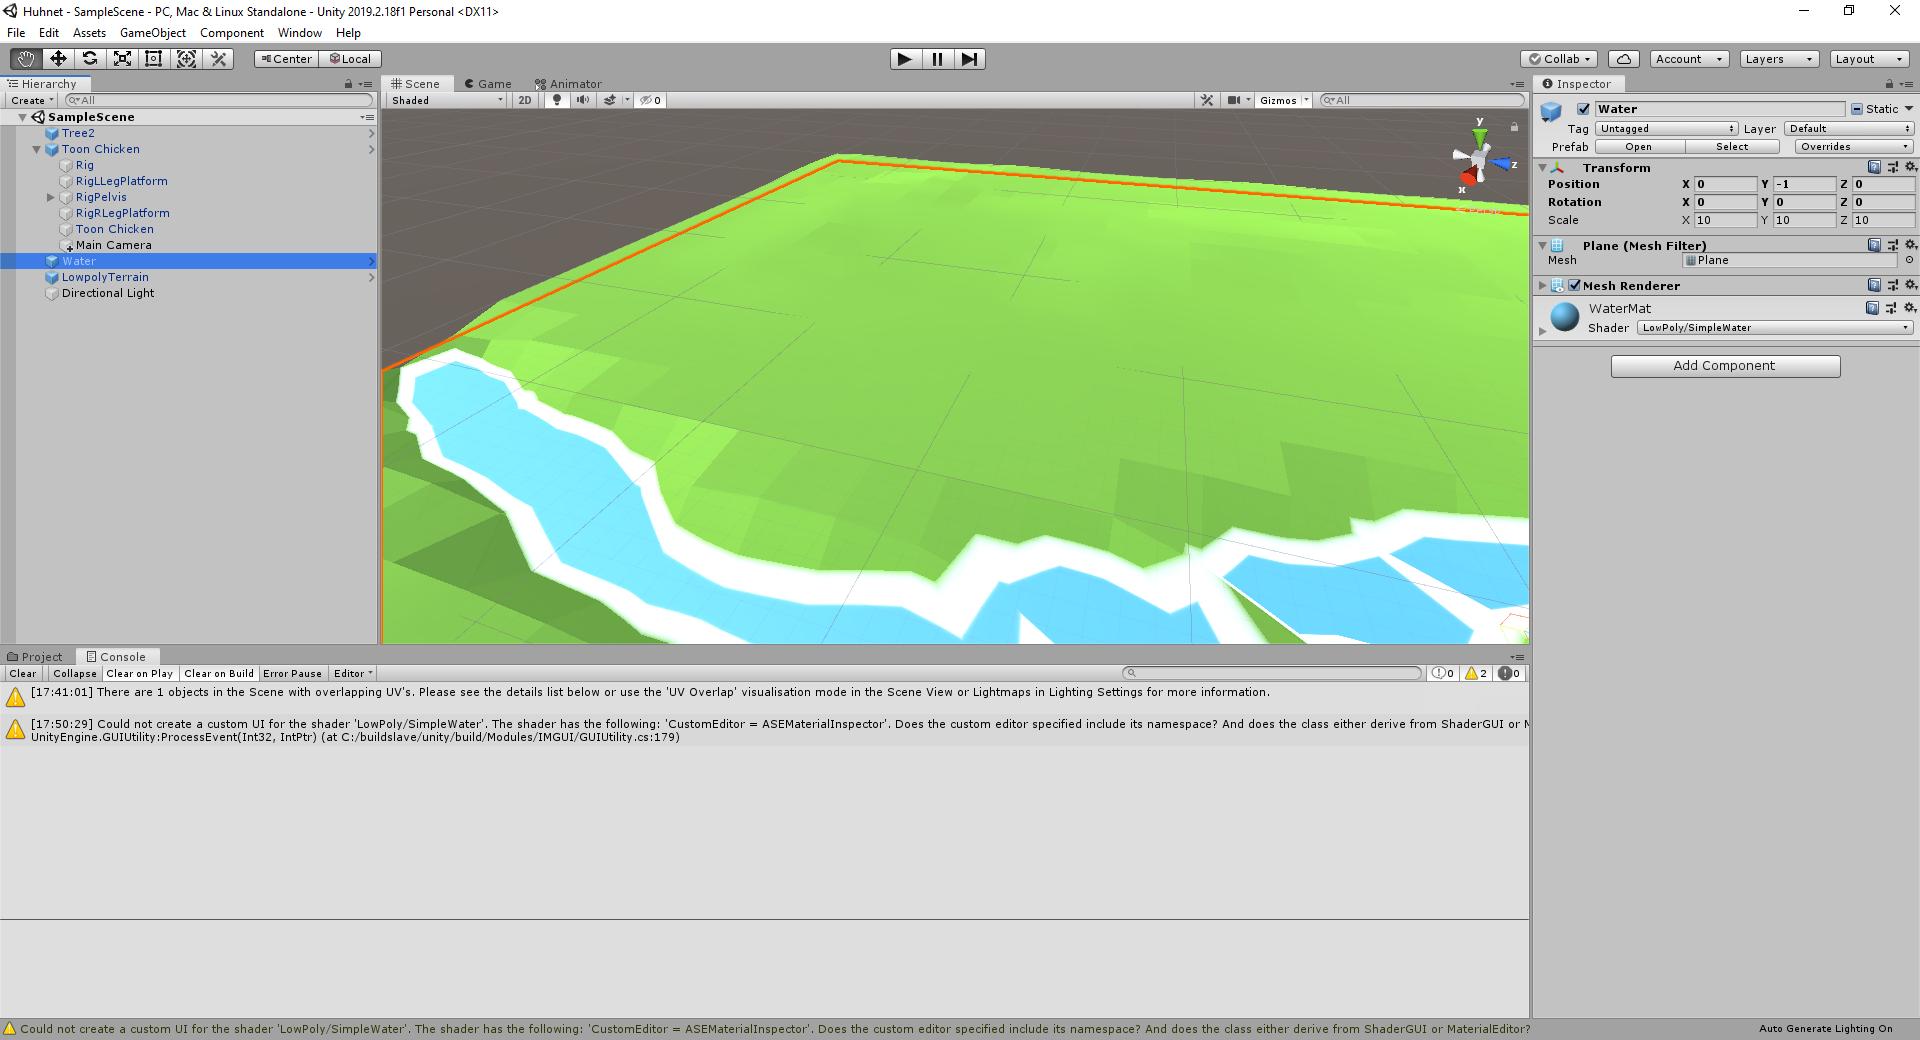
\includegraphics[scale=0.3]{img/unity1.png}
          \caption{Unity Entwicklungsumgebung.}
          \label{fig:unity1}
        \end{figure}
        Zudem bietet Unity nicht nur eine grafische Benutzeroberfläche, 
        sondern auch viele weitere Funktionen, die im Folgenden aufgelistet werden:
        \begin{itemize}
          \item Grafik gemäß dem aktuellen Stand der Technik
          \item Animationen, um Charaktere oder andere Modelle animieren zu können
          \item Physik für das Verhalten von Objekten in einer Welt
          \item Musik und Geräusche, welche Stereofonie ermöglichen
          \item Programmierung, um die einzelnen Entitäten durch eigene Skripte
          zu erweitern
          \item Toolkits für User Interfaces
          \item Unterstützung für Netzwerk- und Multiplayer-Anwendungen
          \item Cross-Plattform-Entwicklung, um die entwickelte Anwendung auf mehrere
          Plattformen zu veröffentlichen
        \end{itemize}
        Unity bietet eine umfangreiche Dokumentation für jede dieser Funktionen.
        Entwickelt werden die sogenannten Skripts, welche dann in der Programmiersprache
        C\# zu verschiedenen Entitäten hinzugefügt werden können. Dementsprechend ist eine
        gewisse Erfahrung in dieser Programmiersprache notwendig, um effektiv Prototypen
        entwickeln zu können. 
        Unity stellt zusätzlich zu ihrem 3D-Editor die 
        Entwicklungsumgebung MonoDevelop zur Verfügung, mit welcher die Skripte 
        geschrieben sowie Fehlersuche und -beseitigung betrieben werden können.
        Durch die umfangreiche Benutzeroberfläche und den Funktionen benötigt Unity jedoch 
        eine lange Einarbeitungszeit. 
        Im Rahmen dieses Forschungsprojektes werden jedoch nicht alle Funktionen,
        die Unity überliefert, benötigt.
        \footnote{Unity Dokumentation | \url{https://docs.unity3d.com/Manual/} (11.11.2020)}
        \\
        Unity ist kostenlos nutzbar und bietet dabei den vollen Funktionsumfang. Betrug der
        Umsatz in den letzten zwölf Monaten jedoch über 100.000\$, muss eine kommerzielle
        Lizenz erworben werden \footnote{Unity Pläne | \url{https://store.unity.com/\#plans-individual} (11.11.2020)}.
        \\
        Die vorliegende Tabelle stellt zusammenfassend die Vor- und Nachteile der Nutzung
        von Unity für das eigene Forschungsprojekt dar (siehe Tabelle \ref{tab:vor-und-nachteile-unity}).
        \begin{table}[h]
          \begin{center}
            \begin{tabular}{| c | c |}
              \hline
              \textbf{Vorteile} & \textbf{Nachteile} \\ \hline
              Stetige Weiterentwicklung & Lange Einarbeitungszeit \\ \hline
              Umfangreicher Funktionsumfang & \\ \hline
              Grafische Benutzeroberfläche inklusive Editor & \\ \hline
              Mitgelieferte Entwicklungsumgebung & \\ \hline
              Cross-Plattform-Entwicklung & \\ \hline
              Kostenlos nutzbar & \\
              \hline
            \end{tabular}
            \caption{Vor- und Nachteile der Unity Engine.\label{tab:vor-und-nachteile-unity}}
          \end{center}
        \end{table}
      \subsubsection{Unreal Engine}
        Die Unreal Engine ist, verglichen mit den anderen Technologien, ähnlich zur 
        Unity Engine. Dennoch hat diese Software einige andere Ansätze. Was sehr ähnlich
        zur Unity Engine ist, ist der weitläufige Funktionsumfang und die grafische 
        Benutzeroberfläche (siehe Abb. \ref{fig:unreal1}). 
        Auch mit Hilfe dieser Technologie lassen sich über 
        einen 3D-Editor Entitäten bearbeiten und in Szenen positionieren.
        \begin{figure}[t]
          \centering
          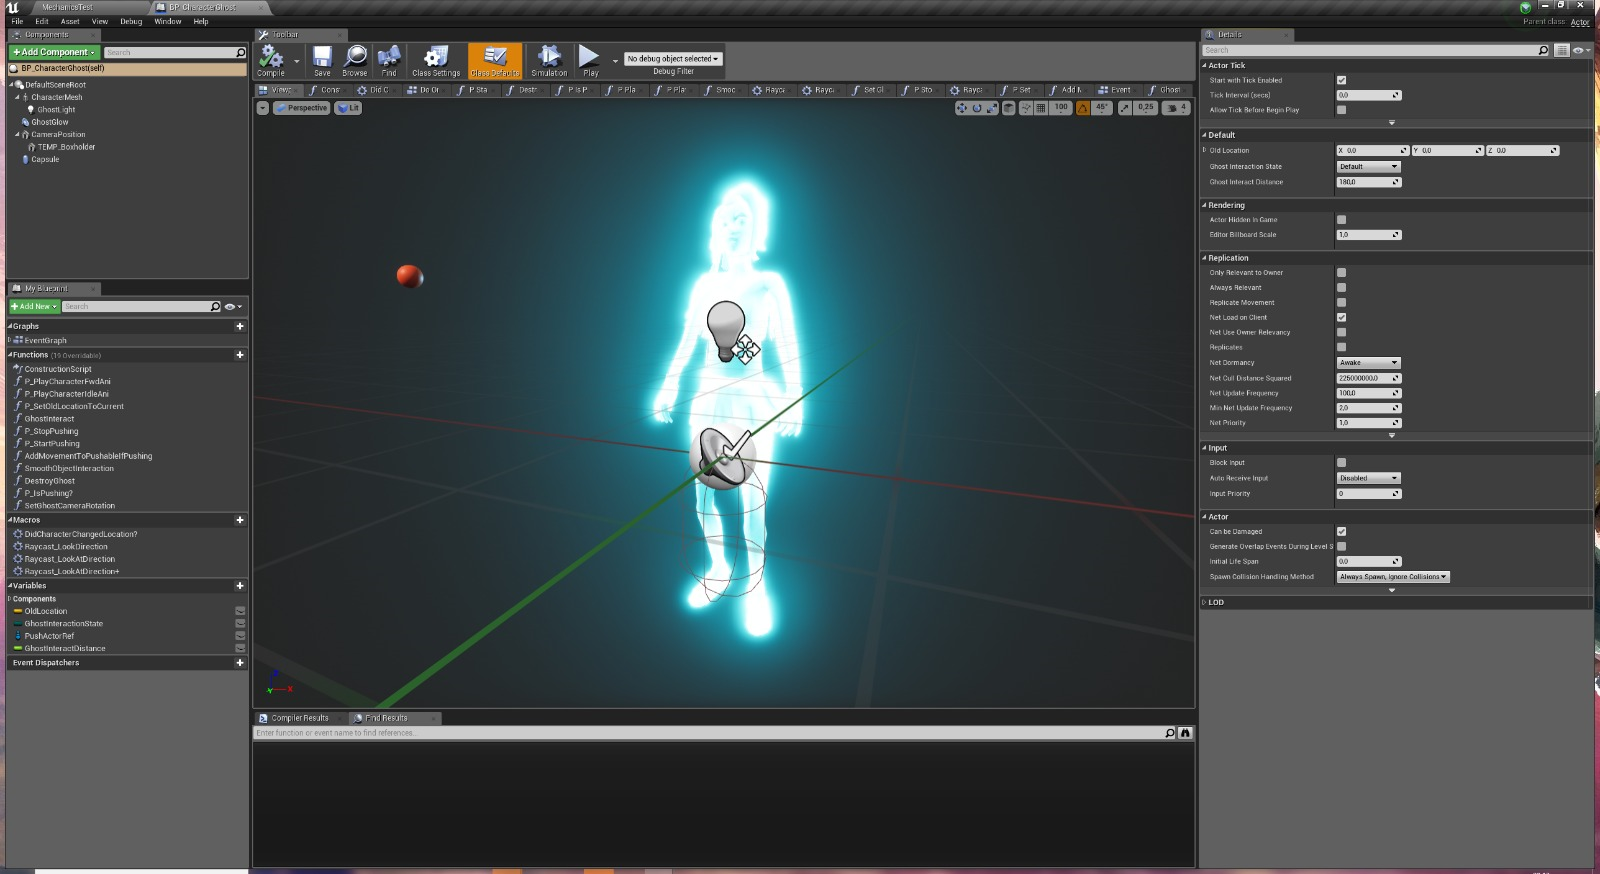
\includegraphics[scale=0.35]{img/unreal1.png}
          \caption{Unreal Engine Entwicklungsumgebung.}
          \label{fig:unreal1}
        \end{figure}
        Zusätzlich verfügt die Unreal Engine,
        für Personen die nicht programmieren können, über ein sogenanntes Blueprint-System
        (siehe Abb. \ref{fig:unreal2}).
        Damit lassen sich per Drag and Drop Algorithmen grafisch zusammenstellen. Somit
        ist Unreal Engine einsteigerfreundlich für Nicht-Entwickler.
        Wenn jedoch komplexere Algorithmen gewünscht sind, wird empfohlen die 
        Programmiersprache C++ anzuwenden. Dazu sollten Kenntnisse im Bereich C++
        mitgebracht werden. Auch dabei muss, wie bereits bei der Unity Engine aufgezeigt
        wurde, eine gewisse Einarbeitungszeit berücksichtigt werden. \\
        \begin{figure}[h]
          \centering
          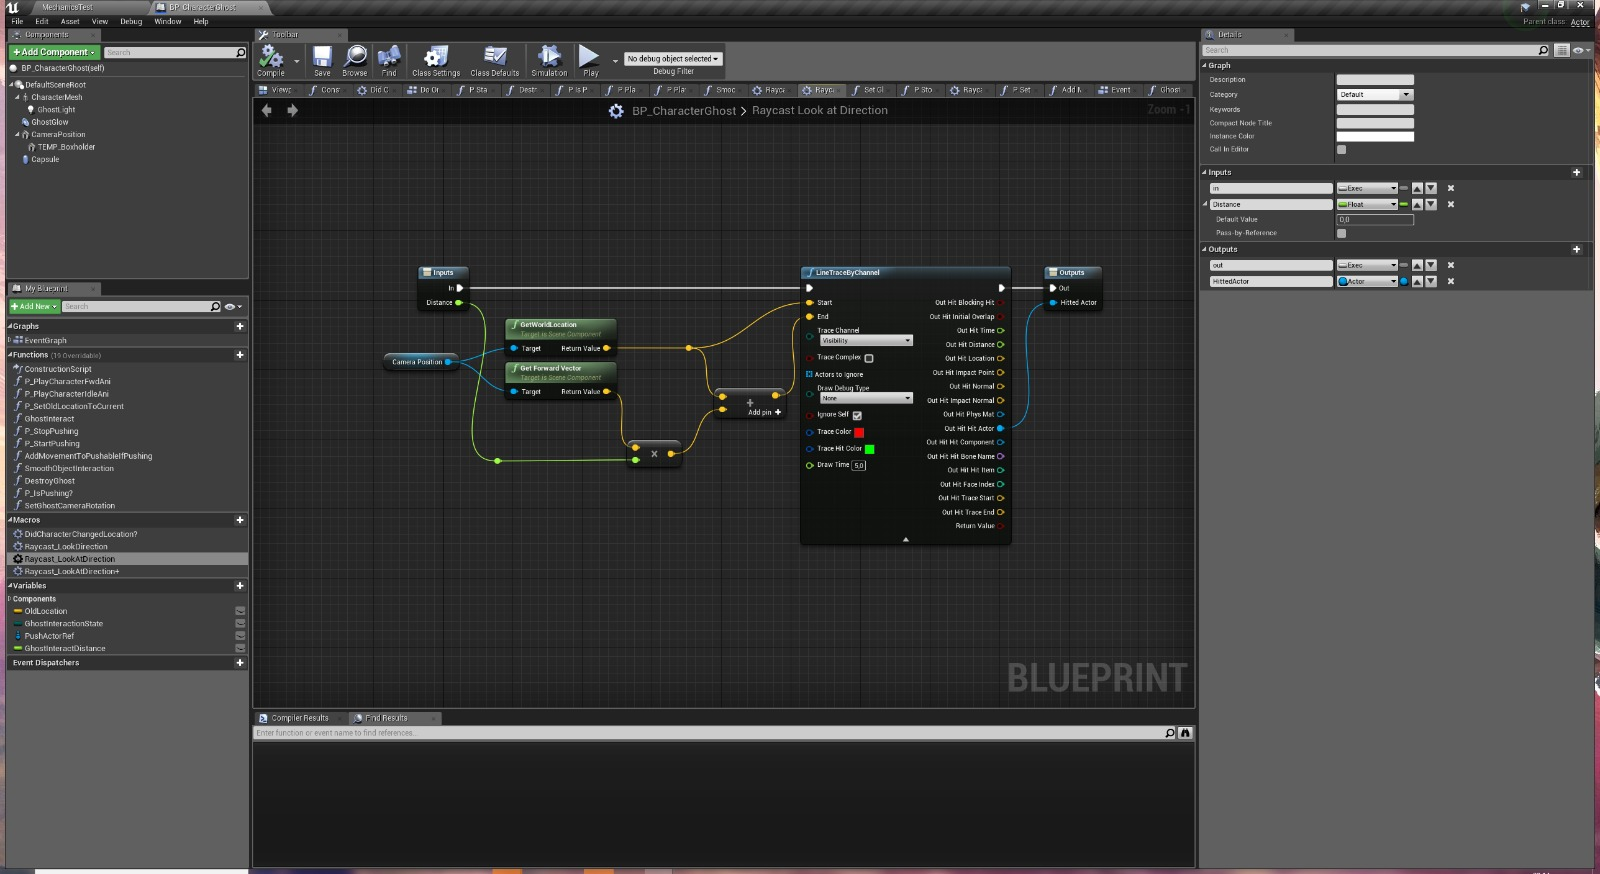
\includegraphics[scale=0.35]{img/unreal2.png}
          \caption{Unreal Engines Blueprint-System.}
          \label{fig:unreal2}
        \end{figure}
        Das Endprodukt einer Software kann daraufhin sowohl auf viele verschiedene Plattformen 
        als auch in das Web portiert werden. Die Entwicklung von Webanwendungen
        in der Unreal Engine ist jedoch nur über eine Erweiterung möglich, welche von 
        der Community entwickelt wird. Darin zeichnet sich nicht unbedingt ein Nachteil ab, 
        kann aber unter Umständen problematisch sein. Dies ist von der Aktivität 
        der Community abhängig, die an dieser Erweiterung arbeitet. Zum aktuellen
        Zeitpunkt wird die Erweiterung von der Community weiterentwickelt
        \footnote{Unreal Engine Dokumentation | \url{https://docs.unrealengine.com/en-US/index.html} (11.11.2020)}.
        \\
        Die Unreal Engine ist ebenfalls kostenlos nutzbar, sofern kein kommerzieller
        Hintergrund bei der Entwicklung einer Anwendung ist\footnote{Unreal Engine Pläne für Nicht-Spiele | \url{https://www.unrealengine.com/en-US/get-now/non-games} (11.11.2020)}.
        \\
        Die vorliegende Tabelle zeigt zusammenfassend die Vor- sowie Nachteile der Unreal
        Engine für dieses Forschungsprojekt auf (siehe Tabelle \ref{tab:vor-und-nachteile-unreal}).
        \begin{table}[h]
          \begin{center}
            \begin{tabular}{| c | c |}
              \hline
              \textbf{Vorteile} & \textbf{Nachteile} \\ \hline
              Stetige Weiterentwicklung & Lange Einarbeitungszeit \\ \hline
              Umfangreicher Funktionsumfang & \\ \hline
              Grafische Benutzeroberfläche inklusive Editor & \\ \hline
              Mitgelieferte Entwicklungsumgebung & \\ \hline
              Cross-Plattform-Entwicklung & \\ \hline
              Blueprint-System für Nicht-Entwickler & \\ \hline
              Kostenlos nutzbar & \\
              \hline
            \end{tabular}
            \caption{Vor- und Nachteile der Unreal Engine.\label{tab:vor-und-nachteile-unreal}}
          \end{center}
        \end{table}
      \subsubsection{React 360}
        React 360 ist ein Framework zur Entwicklung von Cross-Plattform-Anwendungen auf
        Basis von JavaScript. Wie der Name bereits sagt, stammt React 360 von React ab.
        Da das React-Ökosystem eine große Community mit sich bringt, gibt es viele
        Code-Pakete die zur Entwicklung von Webanwendungen mit React genutzt werden können.
        React 360 baut auf Three.js auf, bietet jedoch ein weiteres Abstraktionslevel und
        vereinfacht dadurch die Entwicklung. Durch die JavaScript Syntax Extension (JSX)
        ist es möglich, einfaches HTML mit JavaScript in einer Datei zu kombinieren 
        \footnote{JSX bei React | \url{https://reactjs.org/docs/introducing-jsx.html} (11.11.2020)}.
        Dadurch ist der Programmcode für den Entwickler lesbarer und einfacher nachzuvollziehen.
        Ein Nachteil ist jedoch, dass React 360 keinen 3D-Editor anbietet und dementsprechend
        auch keine grafische Benutzeroberfläche. 3D-Modelle die
        an eine bestimmte Position sollen, müssen über den Programmcode positioniert und
        daraufhin kontrolliert werden. Das bringt einen Mehraufwand mit sich.
        \footnote{React 360 | \url{https://facebook.github.io/react-360/} (11.11.2020)} \\
        React 360-Anwendungen werden mit JavaScript entwickelt, was einen leichten Einstieg
        erlaubt. C\# und C++ sind im Gegensatz zu JavaScript komplexe
        Programmiersprachen. Unter anderem aufgrund der strengen Typsicherung. Dieser
        Punkt ist aber auch für einige Entwickler ein Nachteil von JavaScript. Dieses
        Problem lässt sich aber durch Hilfsmittel für JavaScript und die passende 
        Entwicklungsumgebung beheben. \\
        React 360 ist Open Source und steht unter der BSD-Lizenz. Demnach darf man diese
        Software kostenlos verwenden, verändern und bei Bedarf kommerziell vertreiben. Der
        Vorteil an Open Source Software ist, dass der Quellcode frei einsehbar ist und 
        sich bei Bedarf sogar verändern lässt. Das ist auch einer der Gründe, weshalb
        React und React 360 eine große und aktive Community besitzt. \\
        Nachfolgend können in der vorliegenden Tabelle (siehe Tabelle \ref{tab:vor-und-nachteile-react}) 
        die Vor- und Nachteile für das React 360 Framework als Technologie für dieses 
        Forschungsprojekt festgehalten werden.
        \begin{table}[h]
          \begin{center}
            \begin{tabular}{| c | c |}
              \hline
              \textbf{Vorteile} & \textbf{Nachteile} \\ \hline
              React-Ökosystem & Kein 3D-Editor \\ \hline
              Einsteigerfreundlich & Keine grafische Benutzeroberfläche \\ \hline
              Open Source & \\ \hline
              Kostenlos nutzbar & \\ \hline
              Cross-Plattform-Entwicklung & \\
              \hline
            \end{tabular}
            \caption{Vor- und Nachteile von React 360.\label{tab:vor-und-nachteile-react}}
          \end{center}
        \end{table}
      \subsubsection{A-Frame}
        A-Frame ist, wie React 360, ein Framework, mit welchem WebXR-Anwendungen
        entwickelt werden können. Dazu muss ebenfalls in der Programmiersprache 
        JavaScript entwickelt werden. A-Frame erweitert HTML um eigene 
        HTML-Elemente, was das Benutzen von geometrischen Entitäten oder 3D-Modelle
        vereinfacht (siehe Abb. \ref{fig:aframe1}). Damit schafft A-Frame ein 
        weiteres Abstraktionslevel, was das Programmieren einer VR-Anwendung 
        deklarativ macht. Prototypen lassen sich bereits ohne das Anwenden von 
        JavaScript entwickeln, was vor allem den Einstieg immens vereinfacht.
        \begin{figure}[h]
          \centering
          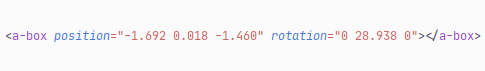
\includegraphics{img/aframe1.png}
          \caption{HTML-Element aus A-Frame.}
          \label{fig:aframe1}
        \end{figure}
        Ein weiterer Vorteil von A-Frame ist die mitgelieferte grafische 
        Benutzeroberfläche die im Browser läuft (siehe Abb. \ref{fig:aframe1-gui}).
        Darüber lassen sich Entitäten positionieren und Komponenten zu diesen 
        hinzufügen. Wie bereits erwähnt verfügt A-Frame über eine aktive und große
        Community und bietet deshalb einen Discord-Server an\footnote{Discord ist eine Software zum Schreiben und Telefonieren. Es können öffentliche Server eingerichtet werden mit verschiedenen Chat-Kanälen, in denen sich ausgetauscht werden kann. | \url{https://discord.gg/tGYjkYr} (12.11.2020)}.
        Auf diesem können jederzeit Fragen zu A-Frame gestellt werden.
        \begin{figure}[h]
          \centering
          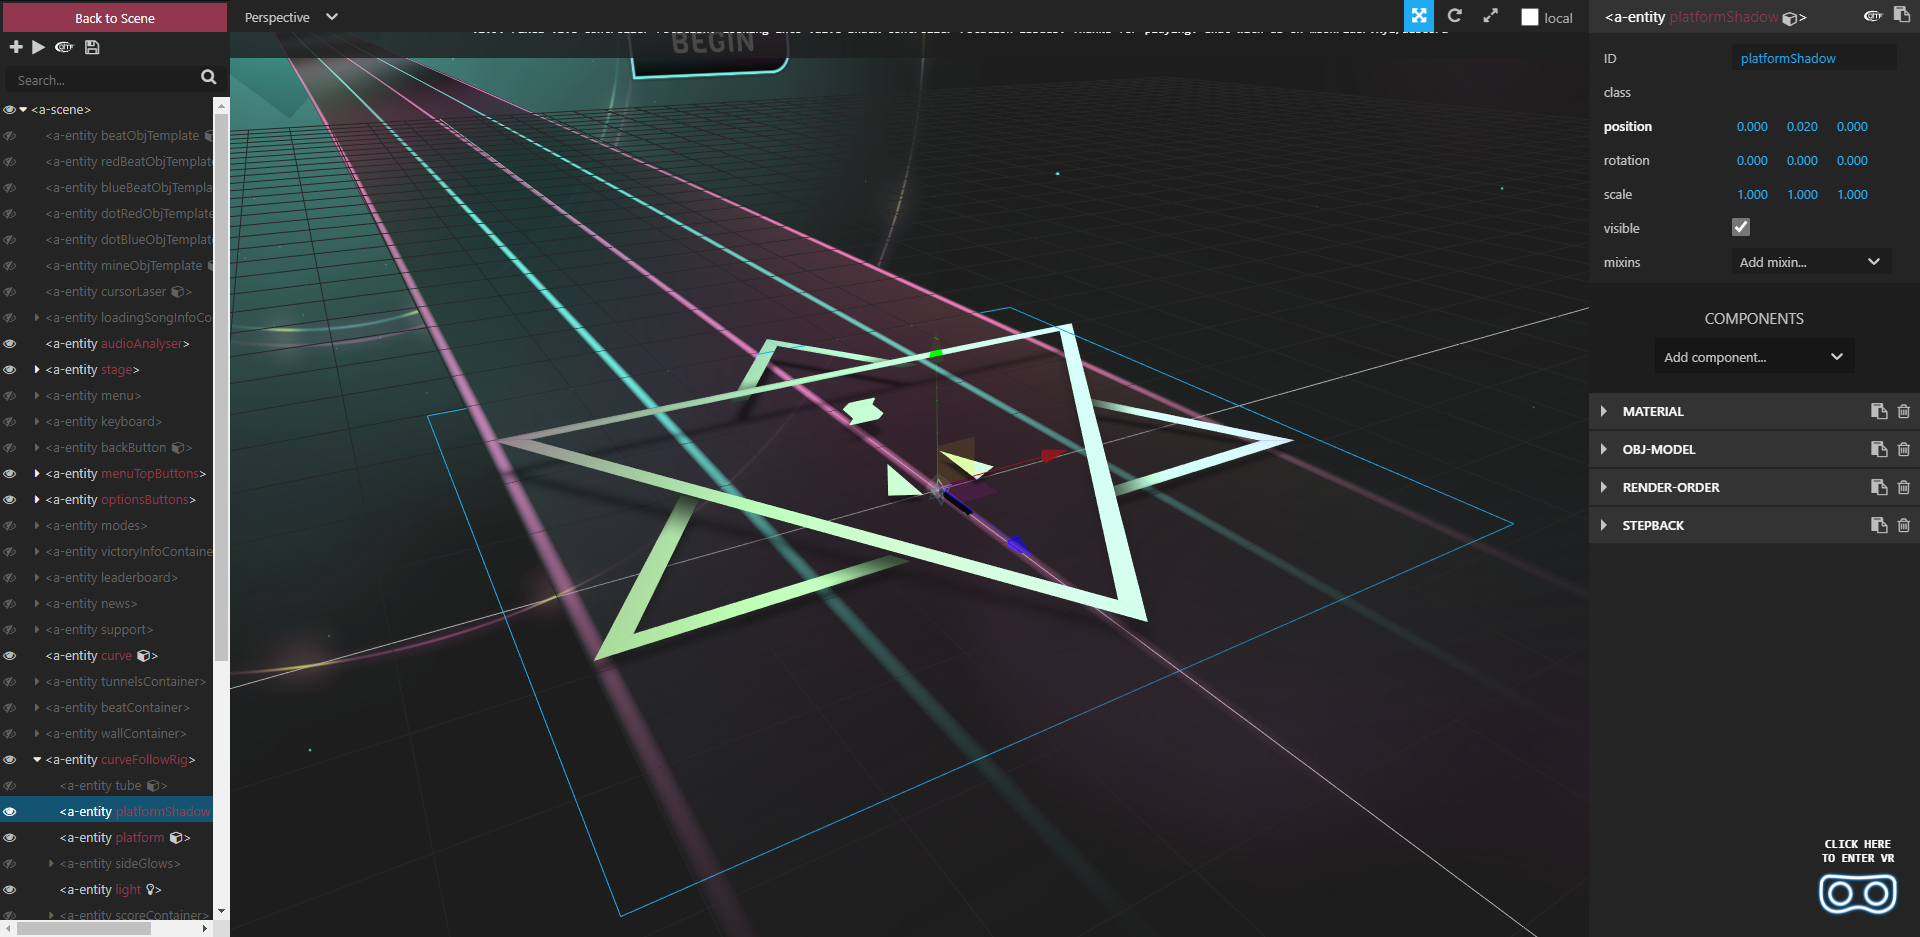
\includegraphics[scale=0.3]{img/aframe-editor.png}
          \caption{Grafische Benutzeroberfläche von A-Frame.}
          \label{fig:aframe1-gui}
        \end{figure}
        A-Frame baut ebenfalls auf Three.js auf, weshalb es auch die Funktionen
        dieser Library mitbringt. Bei Bedarf lässt sich über JavaScript auf 
        den vollen Funktionsumfang von Three.js innerhalb von A-Frame Komponenten
        zugreifen. Das macht das Framework sehr flexibel und mächtig. \\
        A-Frame ist Open Source und steht unter der MIT-Lizenz. Somit kann dieses
        Framework kostenlos und ohne Einschränkungen zur Entwicklung der 
        Prototypen verwendet werden. \\
        In der vorliegenden Tabelle werden die Vor- sowie Nachteile von A-Frame als
        Technologie für dieses Forschungsprojekt aufgezeigt (siehe Tabelle \ref{tab:vor-und-nachteile-aframe}).
        \footnote{A-Frame Dokumentation | \url{https://aframe.io/docs/1.0.0/introduction/}}
        \begin{table}[h]
          \begin{center}
            \begin{tabular}{| c | c |}
              \hline
              \textbf{Vorteile} & \textbf{Nachteile} \\ \hline
              3D-Editor & \\ \hline
              Grafische Benutzeroberfläche & \\ \hline
              Einsteigerfreundlich & \\ \hline
              Keine Programmierkenntnisse notwendig & \\ \hline
              Communityserver & \\ \hline
              Open Source & \\ \hline
              Kostenlos nutzbar & \\ \hline
              Cross-Plattform-Entwicklung & \\ 
              \hline
            \end{tabular}
            \caption{Vor- und Nachteile von A-Frame.\label{tab:vor-und-nachteile-aframe}}
          \end{center}
        \end{table}
      \subsubsection{Three.js}
        Three.js ist eine Library die auf JavaScript basiert und demnach auch
        für diese Programmiersprache vorgesehen ist. Ähnlich wie A-Frame bietet
        Three.js eine Anlaufstelle für ihre Community. Neben einem Discord-Server
        lässt es sich auch über ein Forum austauschen. Auf der Webseite findet man
        auch viele Beispielprojekte, die Three.js nutzen. Darunter finden sich auch
        A-Frame und React 360. \\
        Three.js bietet wie Unity und Unreal Engine vorprogrammierte Funktionen an
        wie Physik, Animationen oder einen 3D-Editor. Der Editor ist jedoch, anders
        als bei A-Frame, nicht im eigenen Projekt integriert, sondern über die
        Webseite von Three.js erreichbar. In diesem Editor können die
        Funktionen anhand einer grafischen Benutzeroberfläche ausprobiert und
        erprobt werden. \\
        Auf der Webseite wird eine eigene Tutorialreihe angeboten in der auch
        auf die Entwicklung von WebVR-Anwendungen eingegangen wird. \\
        Da keine grafische Benutzeroberfläche mitgeliefert wird und alles über den
        Programmcode erstellt werden muss, steigt die Komplexität bei dieser
        Technologie. \\
        Three.js ist Open Source, steht unter der MIT-Lizenz und lässt sich daher
        kostenfrei ohne Einschränkungen nutzen für die Entwicklung der Prototypen.
        \footnote{Three.js Webseite | \url{https://threejs.org/}}
      \subsubsection{Ergebnis}
        Nachfolgend lassen sich in der Tabelle \ref{tab:funktionsumfang-technologien} 
        die Vor- und Nachteile der einzelnen Technologien festhalten.

        \begin{table}[h]
          \begin{center}
            \begin{tabular}{| c | c | c | c | c | c | c |}
              \hline
              & \textbf{Unity} & \textbf{Unreal Engine} & \textbf{React 360} & \textbf{A-Frame} & \textbf{Three.js} \\ \hline
              \textbf{Graf. Benutzeroberfläche} & \checkmark & \checkmark & X & \checkmark & X \\ \hline
              \textbf{3D-Editor} & \checkmark & \checkmark & X & \checkmark &  \checkmark \\ \hline
              \textbf{Einsteigerfreundlich} & X & X & \checkmark & \checkmark & \checkmark \\ \hline
              \textbf{Große Community} & \checkmark & \checkmark & \checkmark & \checkmark & \checkmark \\ \hline
              \textbf{Open Source} & X & X & \checkmark & \checkmark & \checkmark \\ \hline
              \textbf{Kostenlos nutzbar} & \checkmark & \checkmark & \checkmark & \checkmark & \checkmark \\ \hline
            \end{tabular}
            \caption{Funktionsumfang aller Technologien.\label{tab:funktionsumfang-technologien}}
          \end{center}
        \end{table}

        Diese Tabelle zeigt, dass die meisten Vorteile A-Frame und Three.js 
        mitbringen. Da in diesem Forschungsprojekt auch Kentnisse im Bereich
        JavaScript und Webentwicklung mitgebracht werden, spricht dies 
        zusätzlich für die Entwicklung in einer der 
        beiden Technologien. \\
        A-Frame bietet zusätzlich zu Three.js eine grafische Oberfläche, welche
        in jedem Projekt automatisch integriert und über den Browser zu
        bedienen ist. Der volle Funktionsumfang von Three.js ist 
        auch weiterhin in A-Frame
        enthalten, da das Framework auf dieser Library aufbaut. Dadurch, dass
        A-Frame auf ein weiteres Abstraktionslevel setzt und viele vorgefertigte
        Funktionen mitbringt, die in Three.js selbst implementiert werden
        müssten, ist der Einsatz von A-Frame sinnvoll und benötigt keine große
        Einarbeitungszeit. \\
      \subsubsection{Weitere Hilfsmittel}
        Zusätzlich zur Wahl der Technologie lassen sich weitere Hilfsmittel
        in die Entwicklung der Prototypen hinzuziehen. Diese sollen das
        Entwickeln und Verwalten des Codes und der Dateien vereinfachen und
        auch Optimierungen der Peformanz der Anwendung mit sich
        bringen. \\
        Zur Versionsverwaltung wird \textbf{Git} in Kombination mit GitHub
        verwendet. Dadurch können Funktionen implementiert werden ohne den
        aktuellen und lauffähigen Code zu beeinflussen. Bei erfolgreichen
        Tests der neuen Funktionen kann dieser Code in die aktuelle Version
        hinzugefügt werden. Bei Bedarf kann auf alten Code zugegriffen und
        der Code auch auf diesen Stand zurückgebracht werden. \\
        Für eine verbesserte Typsicherheit in JavaScript und produktiveres
        Programmieren wird \textbf{TypeScript} verwendet. So finden Konstrukte
        wie Interfaces aus der objektorientierten Programmierung auch
        Anwendung in JavaScript. Das vereinfacht die Entwicklung mit JavaScript
        und ist skalierbarer. \\
        Das letzte Hilfsmittel welches verwendet wird ist \textbf{Webpack}. Dies
        hilft bei der Optimierung des Codes, da es den gesamten JavaScript-Code
        in eine Datei zusammenfügt und diese keine Leerzeichen, Tabulatoren
        oder Umbrüche beinhaltet. Dadurch ist die Größe der Datei minimiert.
    \subsection{Entwicklung der Prototypen}
      Zu Beginn wird sich mit dem Framework auseinandergesetzt und ein Bereich
      zum Entwickeln geschaffen, in dem verschiedene Ansätze zum Darstellen von
      Gemälden und Archivalien in einer virtuellen Welt ausprobiert werden
      können. \\
      Entwickelt wird in der Entwicklungsumgebung WebStorm von Jetbrains. Die
      VR-Brille, mit der die Anwendungen getestet werden, ist die Oculus Quest,
      welche von der Technischen Hochschule Köln gestellt wird. Diese verwendet
      den Browser Firefox Reality, da dieser viele Funktionen für Entwickler 
      bietet. \\
      Das erste Ziel ist einen technischen Prototypen zu entwickeln, welcher das
      Fortbewegen in der virtuellen Welt durch das Angucken von Objekten ermöglicht.
      Auch sollen Gemälde und deren Beschreibung angezeigt werden können. Sobald
      die ersten technischen Anforderungen erfüllt wurden, 
      sollen weitere Prototypen entwickelt werden.
      \subsubsection{Technischer Prototyp}
        Der erste technische Prototyp soll zeigen, wie eine blickorientierte
        Steuerung und die Gemälde von Lucas Cranach mit Hilfe von A-Frame 
        entwickelt werden können. Dieser soll auch das Fundament für die
        weiteren Prototypen darstellen. \\
        Um den ersten Prototypen zu entwickeln, muss vorerst das Prinzip
        von A-Frame verstanden werden und wie Inhalte mittels HTML
        und JavaScript dargestellt werden können. \\
        Bevor mit der Entwicklung eines Prototypen mit JavaScript begonnen
        werden kann, soll erstmal ein Gemälde von Lucas Cranach innerhalb
        einer virtuellen Welt dargestellt werden. Dafür wird eine statische
        \texttt{index.html}-Datei benötigt, welche die aktuelle stabile 
        Version von A-Frame importiert (siehe Abb. \ref{fig:index1}).
        \begin{figure}[h]
          \centering
          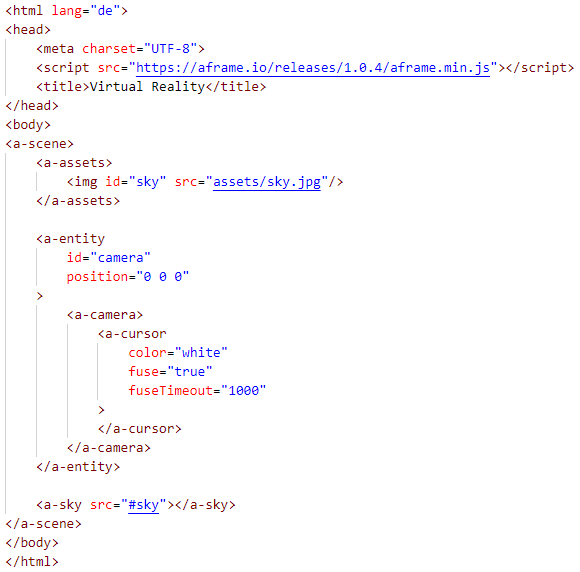
\includegraphics[scale=0.9]{img/coding/index1.png}
          \caption{Erste Version einer \texttt{index.html}-Datei.}
          \label{fig:index1}
        \end{figure}
        Neben den notwendigen HTML-Tags, die für eine valide HTML-Datei
        notwendig sind, kommen \texttt{<a-scene>}, \texttt{<a-assets>},
        \texttt{<a-entity>}, \texttt{<a-camera>}, \texttt{<a-cursor>}
        und \texttt{<a-sky>} hinzu. A-Frame-HTML-Tags lassen sich durch
        das Präfix \texttt{a} erkennen. \\
        Das HTML-Tag \texttt{\textbf{<a-scene>}} ist immer das erste und notwendige
        einer A-Frame-Anwendung. Durch dieses Tag weiß das Framework, 
        dass es sich hierbei um eine A-Frame-Szene handelt. Alles weitere,
        welches im Rahmen von A-Frame entwickelt wird, muss innerhalb
        dieses Tags platziert werden. \\
        \texttt{\textbf{<a-assets>}} beinhaltet alle notwendigen Assets für die 
        VR-Anwendung. Darin können 3D-Modelle oder 
        Bilder (Texturen, Icons, etc.) eingefügt werden. A-Frame empfiehlt,
        sofern möglich, alle Assets die benötigt werden in \texttt{<a-assets>}
        hinzuzufügen, da diese im Cache gespeichert werden und ein Neuladen
        der Anwendung beschleunigt. \\
        Bei \texttt{\textbf{<a-entity>}} handelt es sich um eine einfache Entität,
        welche vorerst keine Darstellung innerhalb der VR-Anwendung haben
        muss. Oft kann dieses Tag auch als Wrapper für mehrere Tags verwendet
        werden. Das hat zum Beispiel den Vorteil, dass nur diese Entität
        angesprochen werden muss, um alle Entitäten innerhalb dieser bewegen
        zu können. Das HTML-Attribut \texttt{id} innerhalb des 
        \texttt{a-entity}-Tags ist keine A-Frame-spezifische Definition,
        sondern hat die selbe Funktion wie in normalem HTML.
        \texttt{position} hingegen gibt die Position als 3D Vektor, 
        relativ zum Nullpunkt der Weltkoordinaten an. In diesem Fall befindet
        sich die Entität genau auf dem Nullpunkt der Weltkoordinaten.
        Das HTML-Tag \texttt{\textbf{<a-camera>}} stellt die Kamera und
        somit die Augen des Benutzers innerhalb der VR-Anwendung dar. Die
        Position der Kamera ist auch die des Benutzers. Eine Kamera
        muss platziert werden, da ansonsten keine virtuelle Welt gesehen
        werden kann. Somit ist dieser HTML-Tag zwingend notwendig. \\
        Innerhalb der \texttt{<a-camera>}-Entität befindet sich 
        \texttt{\textbf{<a-cursor>}}. Mit diesem Cursor kann der Benutzer
        auf bestimmte Entitäten innerhalb einer virtuellen Welt zeigen. Durch
        die Attribute \texttt{fuse} und \texttt{fuseTimeout} lassen sich mit
        diesem auch Entitäten anklicken. A-Frame bietet an der Stelle bereits
        eine Lösung für die blickorientierte Steuerung. Durch 
        \texttt{fuse=true} wird die blickorientierte Steuerung aktiviert.
        \texttt{fuseTimeout="1000"} gibt an, wie viel Millisekunden 
        auf eine Entität geschaut werden muss, 
        damit bei dieser der EventListener
        \texttt{click} ausgelöst wird. Somit muss bei einer Entität ein
        EventListener für \texttt{click} festgelegt werden, damit diese auf
        einen blickorientierten Klick reagieren kann. Das Attribut 
        \texttt{color} legt die Farbe des Cursors fest. \\
        Das HTML-Tag \texttt{\textbf{<a-sky>}} bietet eine fertige Lösung,
        um einen Himmel innerhalb der virtuellen Welt anhand einer Bilddatei
        anzuzeigen. Durch das Attribut \texttt{src="\#sky"} wird die
        Bilddatei mit der ID \texttt{\#sky} aus den Assets geladen. Diese
        Schreibweise ersetzt letztlich die Angabe eines Pfades. \\
        Beim Aufrufen der \texttt{index.html} erscheint folgendes Bild
        (siehe Abb. \ref{fig:vr-welt1}).
        \begin{figure}[h]
          \centering
          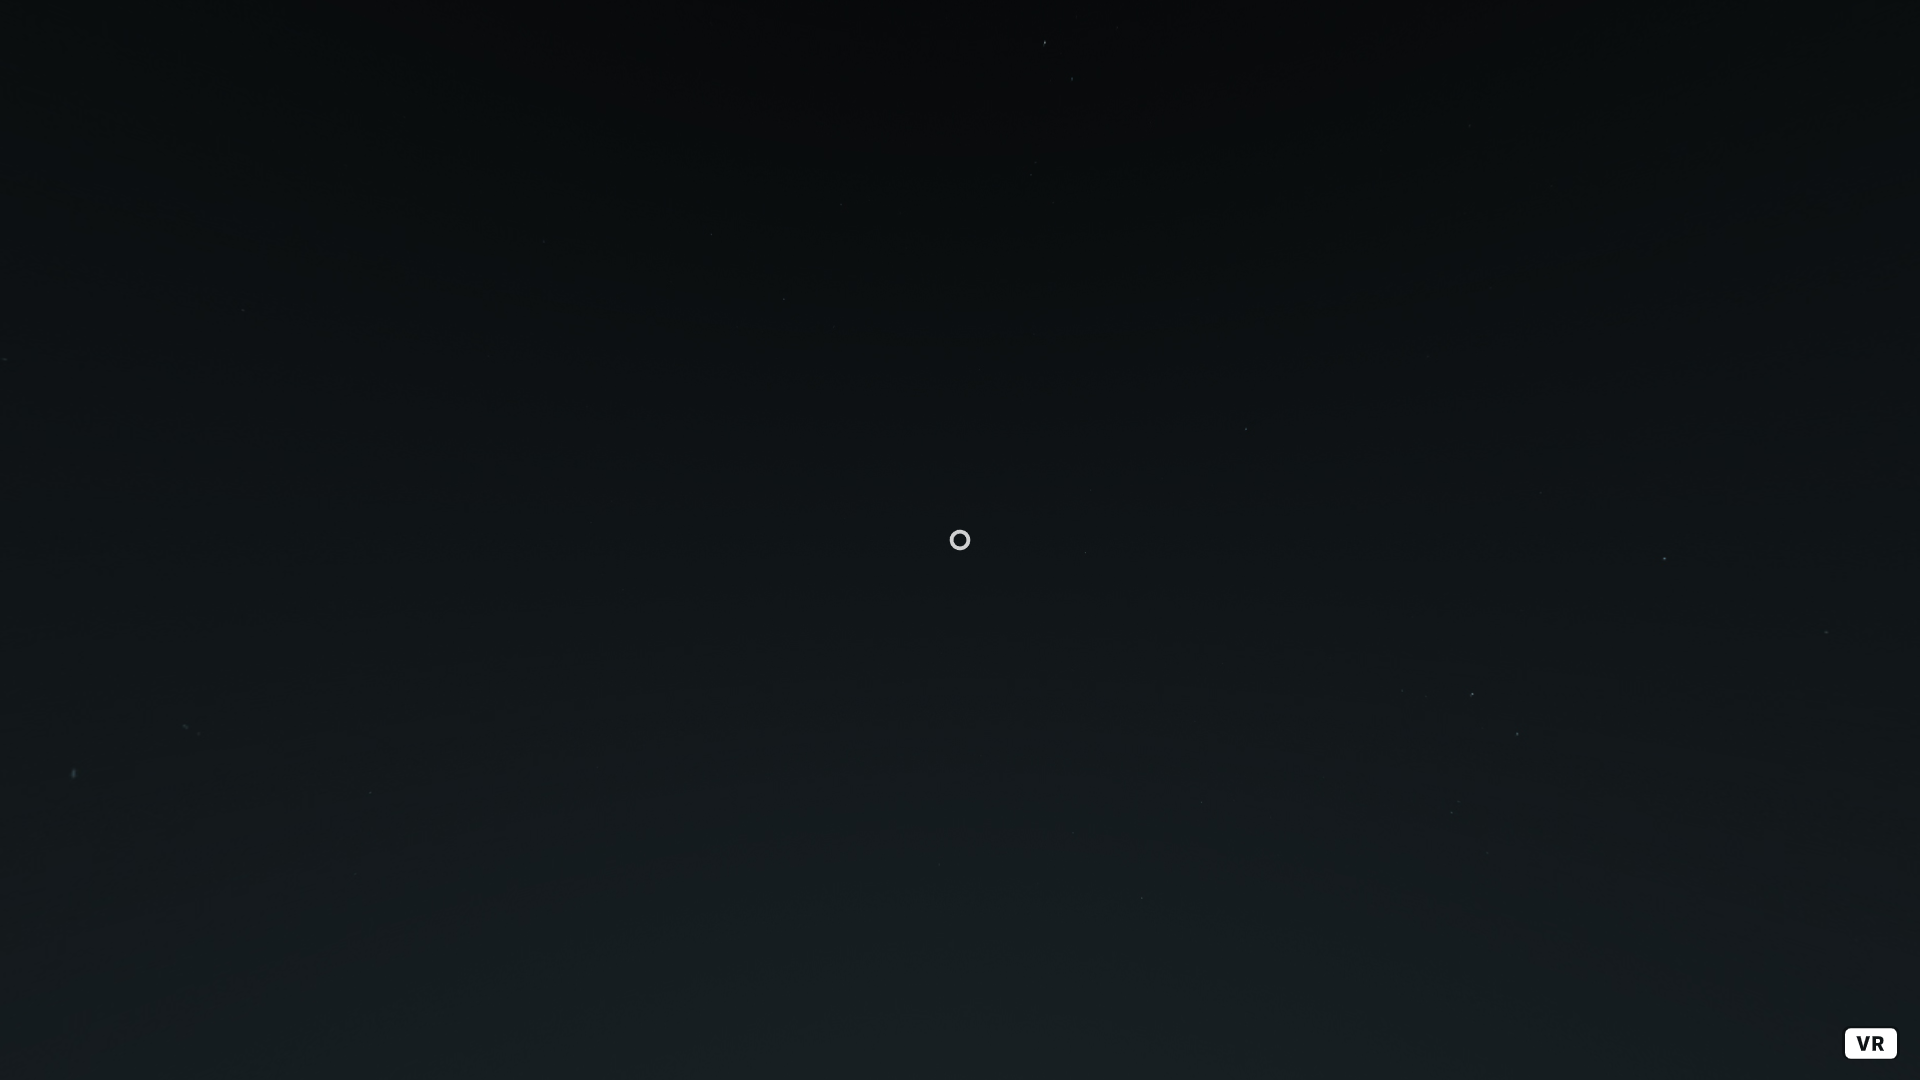
\includegraphics[scale=0.3]{img/coding/vr-welt1.png}
          \caption{Erste virtuelle Welt.}
          \label{fig:vr-welt1}
        \end{figure}
        Der Cursor der Anwendung befindet sich in der Mitte und ist als weißer
        Kreis dargestellt. Unten rechts befindet sich der VR-Button, welcher
        immer von A-Frame mitgerendert wird. Ein Klick auf diesen Button 
        aktiviert den VR-Modus der Webanwendung. \\
        Als nächster Schritt soll ein Gemälde angezeigt werden. In diesem
        Beispiel wird das Gemälde aus dem Cranach Digital Archive
        mit der ID \texttt{DE\_MdbKL\_946} verwendet. A-Frame bietet 
        den HTML-Tag \texttt{\textbf{<a-image>}}, um Bilder anzuzeigen.
        Das Seitenverhältnis der Bilder wird nicht beibehalten, weshalb
        diese durch die Attribute \texttt{width} und \texttt{height} 
        festgelegt werden muss. Das Tag wird einfach innerhalb der
        \texttt{<a-scene>} platziert (siehe Abb. \ref{fig:a-image1}).
        An dieser Stelle bietet A-Frame die Möglichkeit, häufig benutzte
        Eigenschaften von Three.js wie \texttt{height}, \texttt{width}
        oder \texttt{color} über HTML-Attribute festzulegen. Durch diese
        Abstraktion muss nicht über JavaScript die Entität manipuliert
        werden und vereinfacht den Prozess des Prototypings.
        \begin{figure}[h]
          \centering
          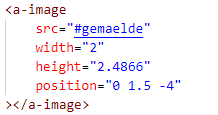
\includegraphics{img/coding/a-image1.png}
          \caption{Image-Tag von A-Frame für das Einbinden von Bildern.}
          \label{fig:a-image1}
        \end{figure}
        Bei den Einheiten innerhalb des Attributs \texttt{position} handelt
        es sich um Angaben in Meter. Die Verschiebung einer Entität ist immer 
        vom Mittelpunkt dieser ausgehend. Betrachtet man das Ganze innerhalb der
        virtuellen Welt, erscheint das Gemälde vor dem Benutzer
        (siehe Abb. \ref{fig:vr-welt2}).
        \begin{figure}[h]
          \centering
          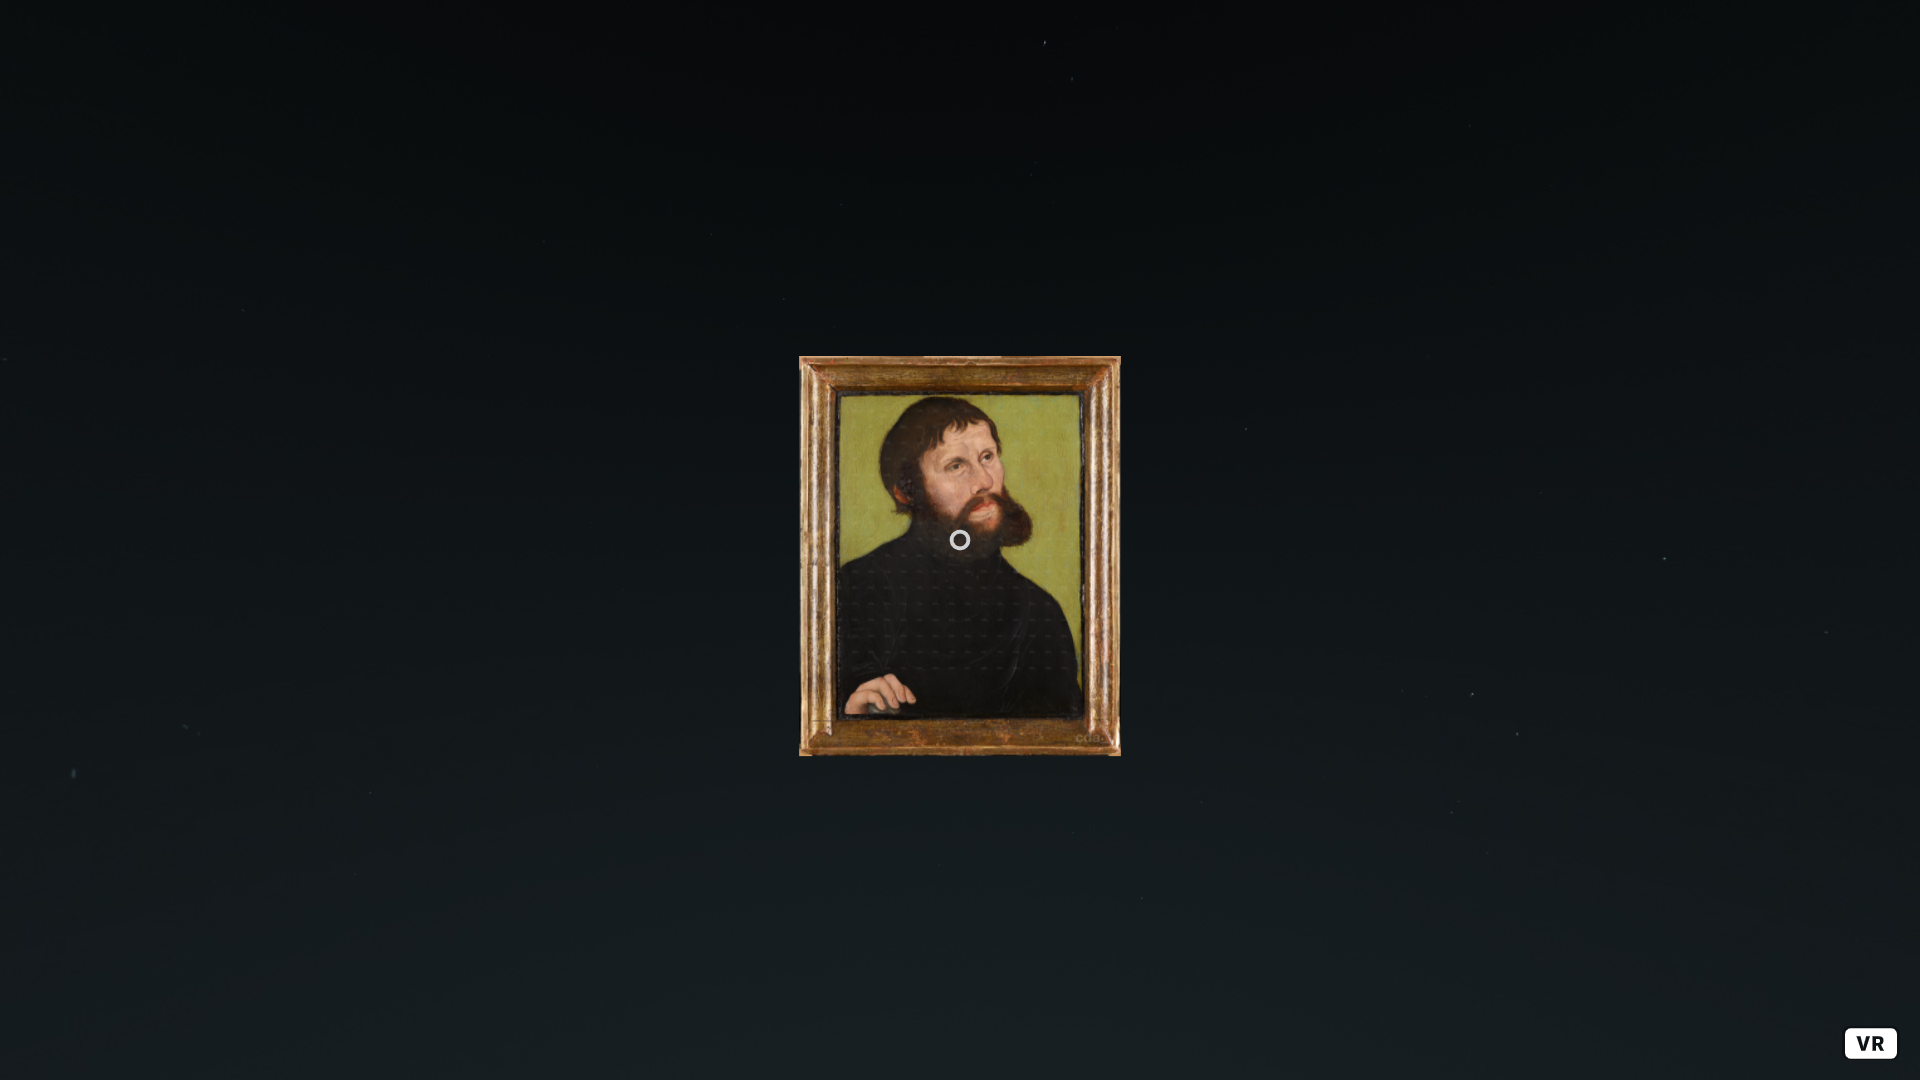
\includegraphics[scale=0.3]{img/coding/vr-welt2.png}
          \caption{Gemälde innerhalb der virtuellen Welt.}
          \label{fig:vr-welt2}
        \end{figure}
        Als nächstes soll eine Steuerung durch das Anschauen von Entitäten
        ermöglicht werden. Da A-Frame bereits eine Lösung für das 
        blickorientierte Klicken zur Verfügung stellt, muss zunächst eine
        Entität erzeugt werden, welches auf Klicken reagiert. Das Framework
        bietet zwei Möglichkeiten EventListener zu registrieren. Die eine
        Möglichkeit besteht darin, die EventListener ebenfalls in HTML
        als Attribut festzulegen. In Abbildung \ref{fig:a-image2} wird
        ein \texttt{click}-EventListener registriert, welches die Komponente 
        sichtbar über \texttt{visible=true} macht. Die zweite Möglichtkeit
        ist das Registrieren eines EventListeners über JavaScript. Diese
        bietet mehr Möglichkeiten und erlaubt den Zugriff auf Three.js
        innerhalb einer Entität.
        \begin{figure}[h]
          \centering
          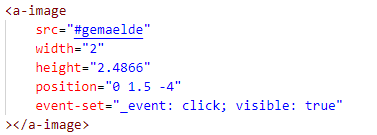
\includegraphics{img/coding/a-image2.png}
          \caption{Event Registrierung innerhalb von HTML.}
          \label{fig:a-image2}
        \end{figure}
        Um einen EventListener mit JavaScript umzusetzen, muss eine Komponente
        entwickelt werden. Komponenten in A-Frame sind wiederverwendbare
        Code-Module, welche zu beliebigen Entitäten hinzugefügt werden
        können. Diese Entitäten übernehmen dann die Logik der Komponente.
        Eine Komponente hat folgenden Aufbau (siehe Abb. \ref{fig:komponente1}).
        \begin{figure}[h]
          \centering
          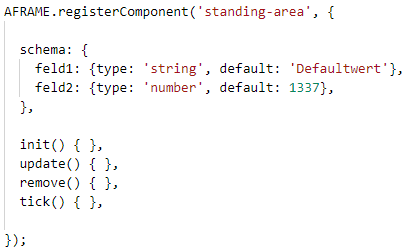
\includegraphics{img/coding/komponente1.png}
          \caption{Aufbau einer Komponente in A-Frame.}
          \label{fig:komponente1}
        \end{figure}
        Um auf A-Frame Funktionen innerhalb der TypeScript-Datei zugreifen
        zu können, muss A-Frame zuerst mit einem Packetmanager wie yarn
        oder npm installiert werden. Aufgrund dessen kann die Importierung
        von A-Frame innerhalb der HTML-Datei entfernt werden, da nun
        nurnoch die \texttt{bundle.js}, welche von Webpack generiert wird,
        importiert werden muss. Diese beinhaltet jeglichen Code, auch den
        der importierten Module innerhalb einer Komponente. \\
        Die in Abbildung \ref{fig:komponente1} gezeigte Komponente lässt
        sich dann über HTML einer Entität hinzufügen 
        (siehe Abb. \ref{fig:komponente2}).
        \begin{figure}[h]
          \centering
          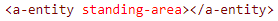
\includegraphics{img/coding/komponente2.png}
          \caption{A-Frame Entität mit hinzugefügter Komponente.}
          \label{fig:komponente2}
        \end{figure}
        Mit \texttt{AFRAME.registerComponent(...)} wird eine
        Komponente für A-Frame erstellt. 
        Das erste Argument ist vom Typ \texttt{string}
        und beinhaltet den Namen der Komponente. Das zweite Argument
        ist ein Objekt, welches die Lifecycle-Methoden und ein Schema 
        einer A-Frame Komponente enthält. \\
        Das Feld \texttt{\textbf{schema}} gibt an, welche Werte
        innerhalb des HTML über das Attribut \texttt{standing-area} 
        in die Komponenten hineingeben werden können. \texttt{feld1}
        und \texttt{feld2} sind die Namen der Eigenschaften. Mit \texttt{type}
        lässt sich der Typ für den Wert festlegen und \texttt{default}
        gibt einen Standardwert zurück, sofern keine Information zu dieser
        Eigenschaft mitgegeben wurde. In Abbildung \ref{fig:komponente2} müsste
        das Attribut um \texttt{standing-area="feld1: Hallo!; feld2: 1338"}
        erweitert werden, damit der Standardwert überschrieben und ein
        neuer hineingegeben wird. Die Werte in \texttt{schema} können dann
        über \texttt{this.data.feld1} oder \texttt{this.data.feld2} 
        innerhalb der Komponente aufgerufen werden. \\
        Die \texttt{\textbf{init}}-Methode wird beim ersten Laden einer
        Entität mit dieser Komponente ausgeführt. Darin lassen sich
        Werte festlegen, die sich im Laufe der Anwendung nicht mehr 
        verändern. \\
        Die \texttt{\textbf{update}}-Methode wird einmalig nach der
        \texttt{init}-Methode ausgeführt und immer, wenn sich Attribute
        der Entität verändern. \\
        Wird die Entität und ihre Komponente gelöscht, wird einmalig
        die \texttt{update}-Methode ausgeführt. \\
        Die \texttt{\textbf{tick}}-Methode ist abhängig von der Bildrate der
        Anwendung. Beträgt die FPS (Bilder pro
        Sekunde) der Anwendung 60, dann wird diese Methode 60 mal ausgeführt. \\
        Um das Teleportieren eines Benutzers auf die Position der Entität, 
        welche angeguckt wird, umzusetzen, wird eine \texttt{<a-box>}
        verwendet. Diese erhält die Komponente \texttt{standing-area}
        (siehe Abb. \ref{fig:standing-area1}).
        \begin{figure}[h]
          \centering
          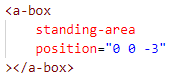
\includegraphics{img/coding/standing-area1.png}
          \caption{a-box mit der Komponente \texttt{standing-area}.}
          \label{fig:standing-area1}
        \end{figure}
        Der Code innerhalb der Komponente \texttt{standing-area} sieht
        wie folgt aus (siehe Abb. \ref{fig:standing-area2}).
        \begin{figure}
          \centering
          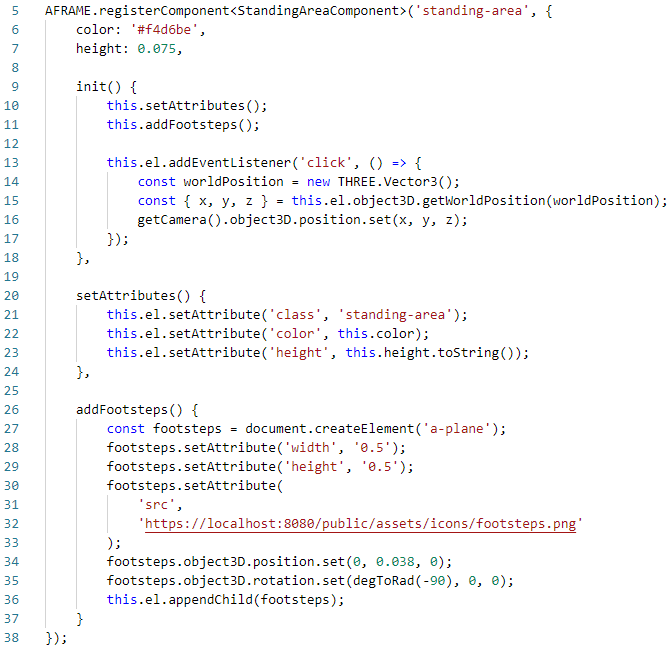
\includegraphics{img/coding/standing-area2.png}
          \caption{TypeScript-Code der Komponente \texttt{standing-area}.}
          \label{fig:standing-area2}
        \end{figure}
        In diesem Beispiel zeigen sich wieder einige Vereinfachungen
        die A-Frame bietet. Soll die Oberflächentextur einer
        Entität verändert werden, so lässt sich das über das HTML-Attribut
        \texttt{src} machen
        (siehe Abb. \ref{fig:standing-area2}, Zeile 30-33). 
        Diese Schreibweise erinnert an das klassische
        HTML-Attribut von einem \texttt{img}-Tag.
        HTML-Attribute, wie \texttt{width},
        \texttt{height} oder \texttt{src} können auch über den Code
        festgelegt werden 
        (siehe Abb. \ref{fig:standing-area2}, Zeile 28-33). \\
        A-Frame Tags lassen sich über JavaScript wie normale HTML-Tags
        generieren und auch beispielsweise mit der Methode \texttt{querySelector}
        selektieren
        (siehe Abb. \ref{fig:standing-area2}, Zeile 27). Über \texttt{this.el}
        lässt sich auf die Entität der Komponente zugreifen. \\
        \texttt{color} legt die Farbe
        einer Entität fest und
        \texttt{color} und \texttt{height} 
        (siehe Abb. \ref{fig:standing-area2}, Zeile 6-7)
        sind zwei selbst festgelegte
        Eigenschaften, welche nicht zwingend in einer A-Frame Komponente
        vorhanden sein müssen. Selbst festgelegte Eigenschaften können
        auch genutzt werden, um den state (Zustand) einer Komponente
        zu speichern. \texttt{color} gibt die Farbe der \texttt{<a-box>}
        an und \texttt{height} die Höhe. \\
        Die Komponente \texttt{standing-area} führt in ihrer \texttt{init}-
        Methode zunächst die beiden internen Methoden \texttt{setAttributes}
        und \texttt{addFootsteps} aus. Erste fügt die notwendigen
        Attribute hinzu, im das Erscheingungsbild der Entität in der
        virtuellen Welt festzulegen. \texttt{class} hingehen ist nicht
        zwingend notwendig, erleichtert jedoch zukünftig das selektieren
        dieser Entität. Die zweite Methode erzeugt das Element 
        \texttt{<a-plane>}
        (siehe Abb. \ref{fig:standing-area2}, Zeile 27). 
        Dabei handelt es sich um eine zweidimensionale
        Fläche. Durch das Attribut \texttt{src} erhält es Fußabdrücke
        als Textur (siehe Abb. \ref{fig:standing-area2}, Zeile 30-33).
        Anders als die Attribute \texttt{height} oder \texttt{width},
        sollen laut A-Frame Eigenschaften wie position und rotation,
        sofern diese über den Code angegeben oder verändert werden,
        über Three.js manipuliert werden
        \footnote{A-Frame Best Practices | \url{https://aframe.io/docs/1.0.0/introduction/best-practices.html} (17.11.2020)}.
        Dies ist schneller als über HTML und spart Leistung ein. \\
        Das \texttt{<a-plane>}-Tag wird etwas über die \texttt{<a-box>}
        positioniert. Dadurch, dass das Element der \texttt{<a-box>} angehängt
        wird, befindet sich dieses Element im DOM innerhalb des \texttt{<a-box>}
        -Tags. Wenn sich Entitäten innerhalb einer anderen Entität befinden,
        werden deren Positionsangaben relativ zum Mutterelement angegeben
        (siehe Abb \ref{fig:standing-area2}, Zeile 35-36). \\
        Zuletzt wird in der \texttt{init}-Methode der \texttt{click}-EventListener
        hinzugefügt (siehe Abb. \ref{fig:standing-area2}, Zeile 13-17).
        Durch den Aufruf von \texttt{.object3D} eines HTML-Elements kann
        auf die Object3D Repräsentation von Three.js zugegriffen werden.
        Bei einem Klick auf die Entität wird die aktuelle Weltposition
        ausgelesen und der Kamera hinzugefügt 
        (siehe Abb. \ref{fig:standing-area2}, Zeile 15-16). Die \texttt{getCamera}
        -Methode ist eine globale Methode, welche das Kamera-Element 
        zurückliefert. \\
        Somit wird der Benutzer nun zu den Standfläche teleportiert, wenn
        er diese für 1 Sekunde anschaut 
        (siehe Abb. \ref{fig:standing-area3}).
        \begin{figure}[h]
          \centering
          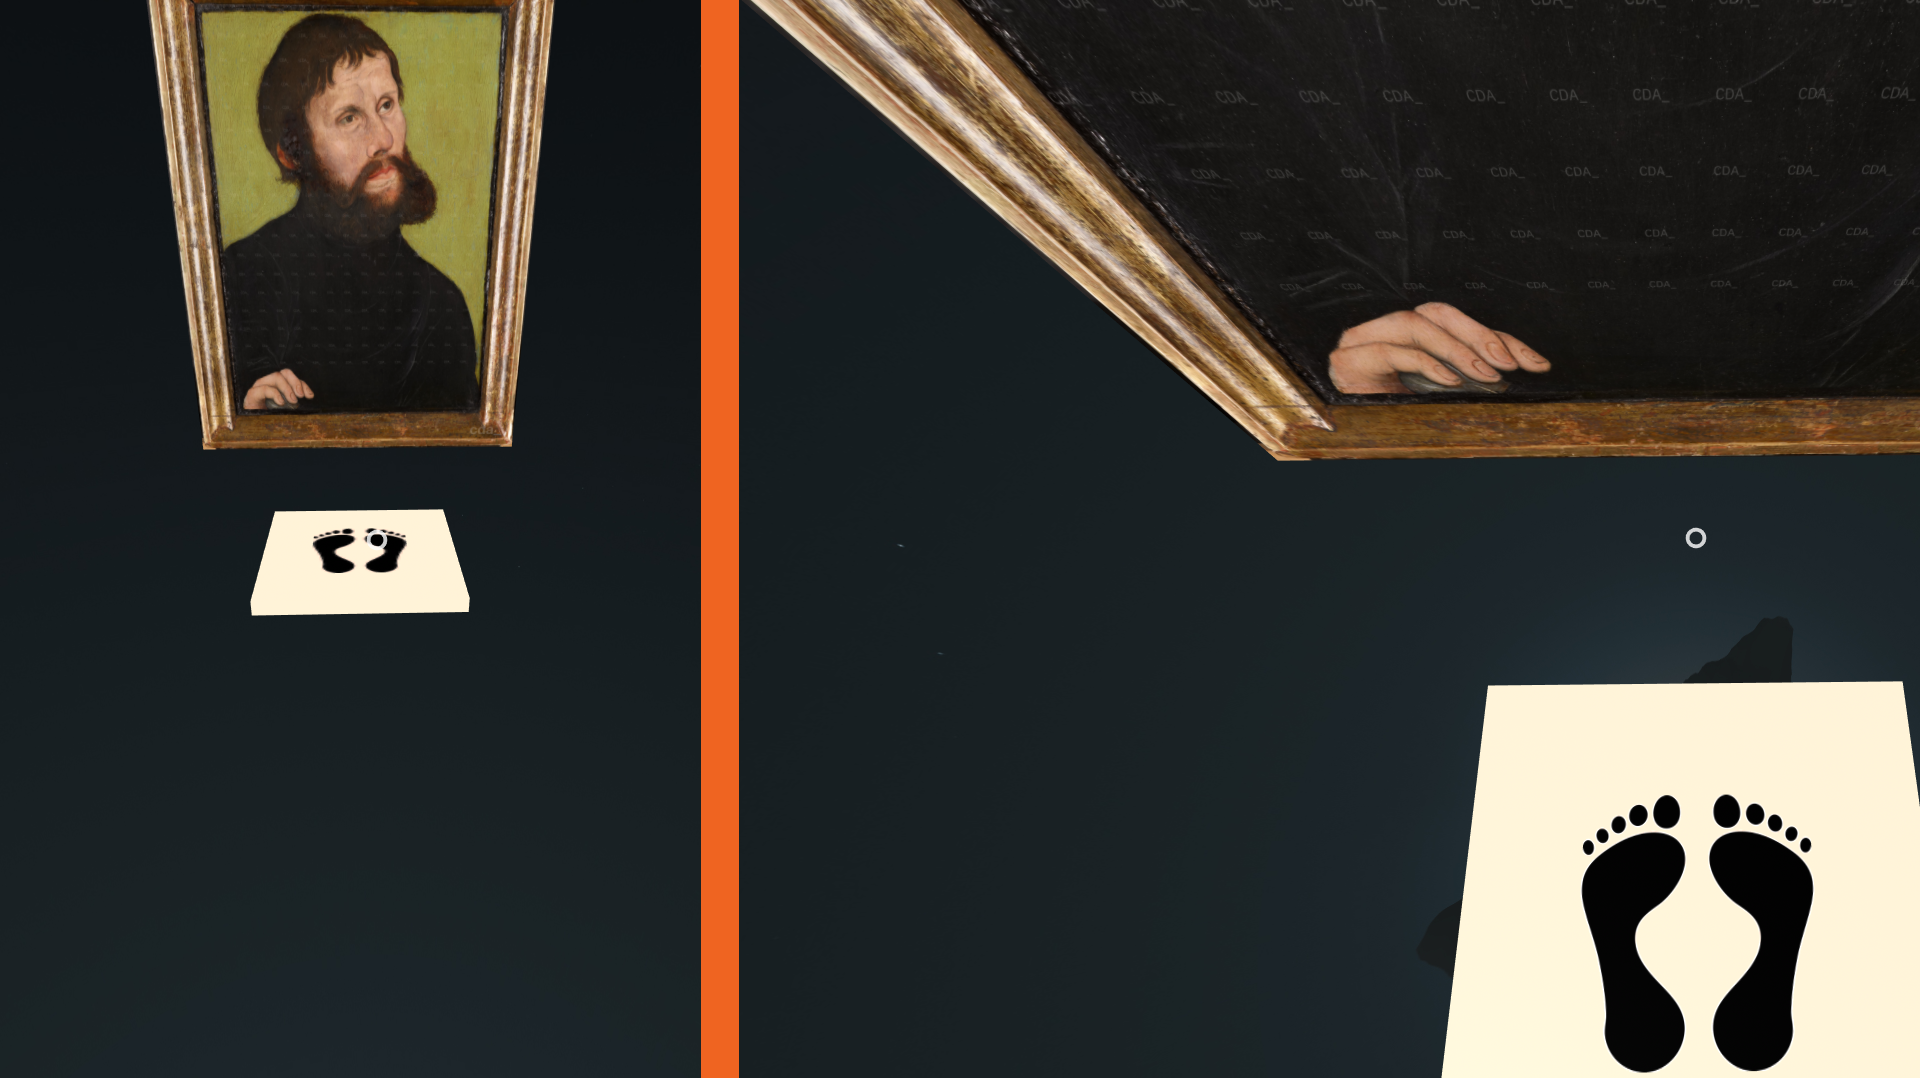
\includegraphics[scale=0.3]{img/coding/standing-area3.png}
          \caption{Funktionsfähige Standing Area zum Teleportieren.}
          \label{fig:standing-area3}
        \end{figure}
        Auf der linken Seite der Abbildung \ref{fig:standing-area3} schaut
        der Benutzer auf die Standing Area. Rechts daneben zeigt die neue
        Position des Benutzers auf der Standing Area an. Er befindet sich
        nun vor dem Gemälde und kann dies genauer betrachten. \\
        Damit der Benutzer nicht vor einem Gemälde ohne Informationen
        steht, soll neben dem Gemälde einige Details zu diesem angezeigt
        werden. A-Frame bietet das Tag \texttt{<a-text>}, womit man 
        zweidimensionalen Text in der virtuellen Welt anzeigen lassen kann.
        Damit die Inhalte nicht unübersichtlich werden, wurden die Inhalte
        auf Autor, Datierung, Zuschreibung und Bildträger beschränkt. 
        Über das Attribut \texttt{value} kann ein Text festgelegt werden,
        welches in der virtuellen Welt angezeigt wird
        (siehe Abb. \ref{fig:description2}). \\
        \begin{figure}
          \centering
          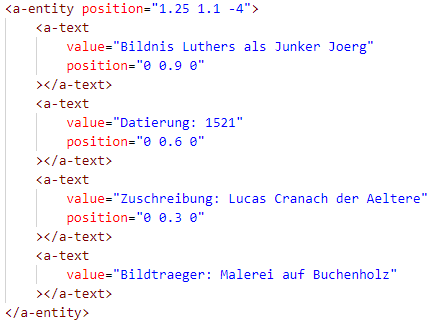
\includegraphics{img/coding/description2.png}
          \caption{Beschreibung zum Gemälde der ID \texttt{DE\_MdbKL\_946}.}
          \label{fig:description2}
        \end{figure}
        Durch die richtige Positionierung erscheint der Text neben
        dem Gemälde (siehe Abb. \ref{fig:description1}).
        \begin{figure}
          \centering
          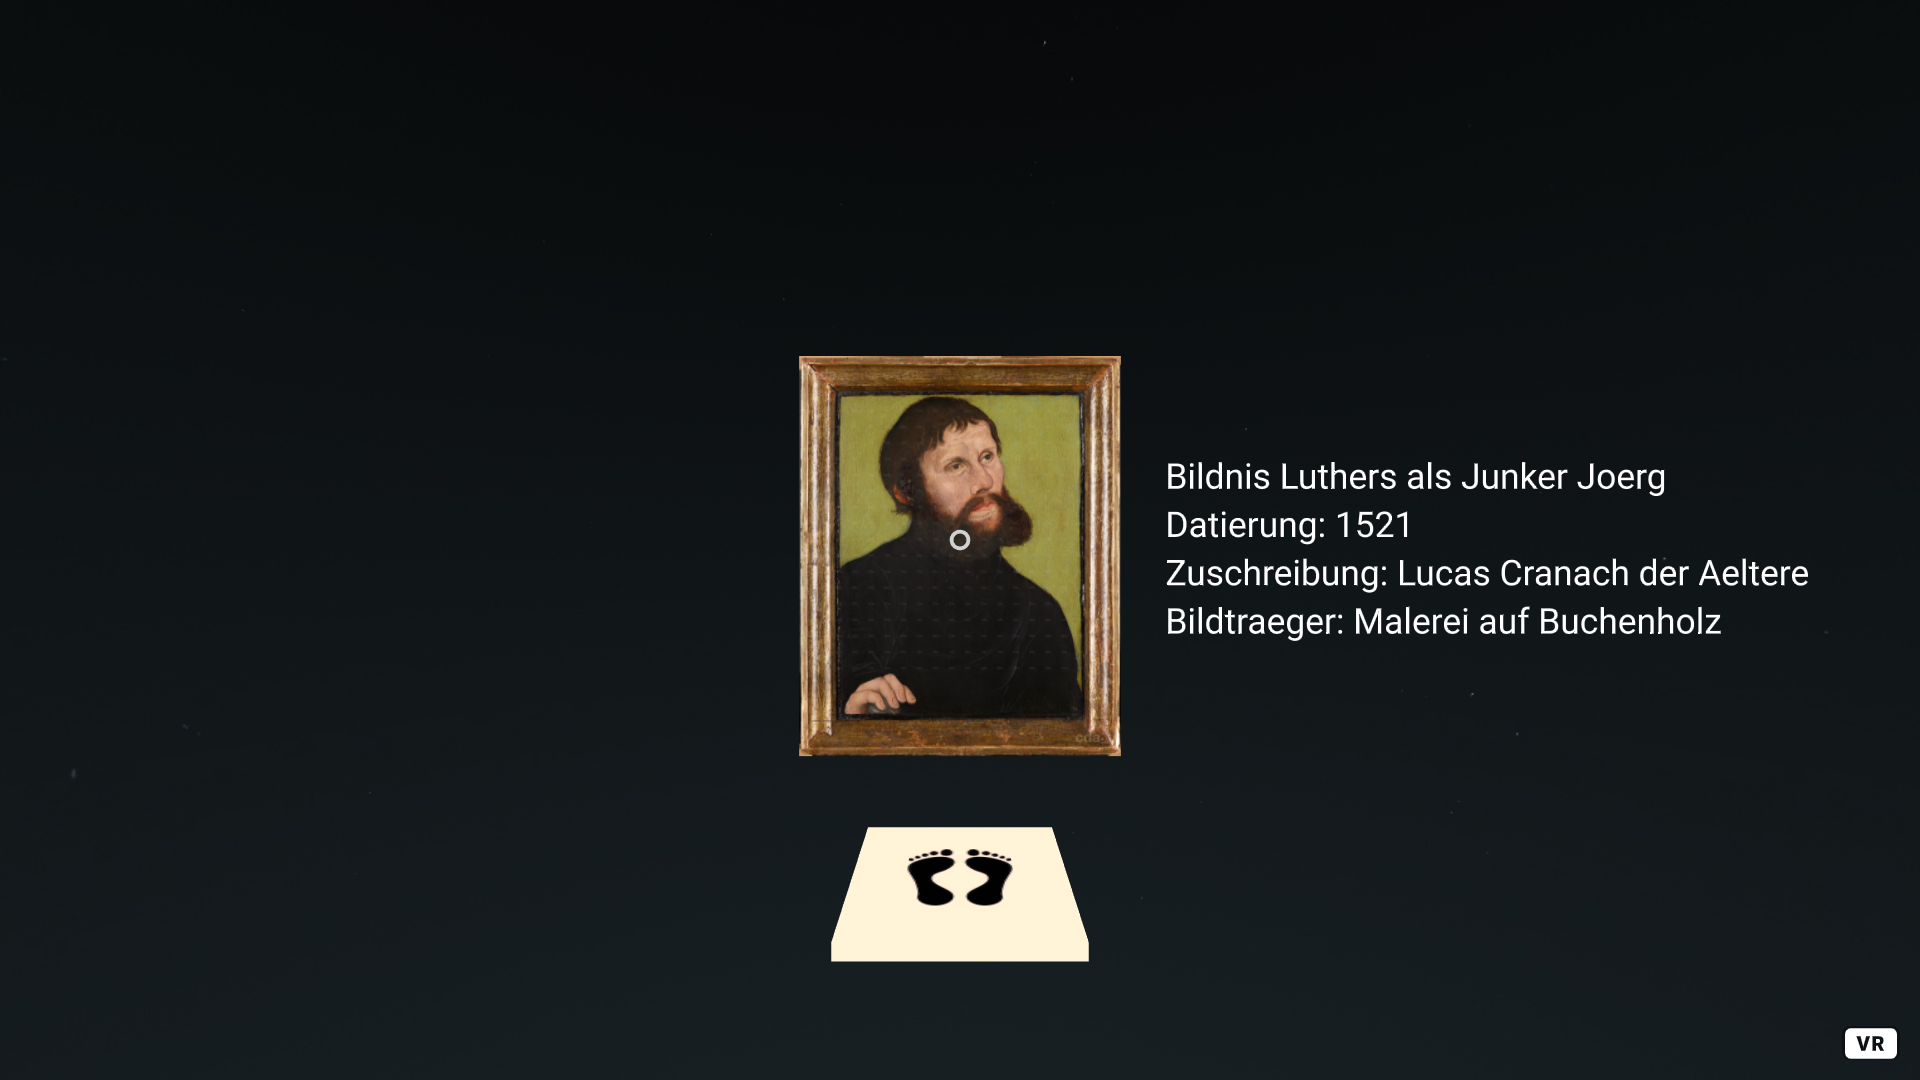
\includegraphics[scale=0.3]{img/coding/description1.png}
          \caption{Beschreibung zum Gemälde der ID \texttt{DE\_MdbKL\_946} innerhalb der virtuellen Welt.}
          \label{fig:description1}
        \end{figure}
        Neben den Informationen zu einem Gemälde besitzt dieses im Cranach
        Digital Archive auch mehrere Detailaufnahmen. Diese zeigen besondere
        Stellen im Gemälde auf und bieten eine hochauflösende Nahaufnahme.
        Für den Benutzer soll es die Möglichkeit geben diese auch ansehen zu
        können. Dafür soll ein Button unter den Informationen angezeigt werden,
        welcher sich anklicken lässt. Wurde dieser angeklickt, erscheinen
        Punkte auf dem Gemälde, die dort positioniert sind, an denen sich
        die Nahaufnahmen befinden. Wird einer dieser Punkte angeklickt, 
        erscheint statt dem Gemälde die Nahaufnahme vor dem Benutzer. Um
        diese Funktion umzusetzen, müssen zwei weitere Komponenten entwickelt
        werden. Zum einen der Button, mit welchem die Punkte innerhalb
        des Gemäldes erscheinen und zum anderen die Punkte selbst, welche
        das Gemälde durch eine Nahaufnahme ersetzen. Dafür muss das
        \texttt{src}-Attribut des Gemäldes verändert werden. A-Frame reagiert
        auf Veränderungen innerhalb des DOM und aktualisiert die Anwendung
        in Echtzeit. \\
        Mittlerweile wird der technische Prototyp komplexer und eine
        Datenstruktur für die Gemälde wird notwendig, da mehrere Nahaufnahmen
        zu einem Gemälde existieren. Auch die Punkte, die auf dem Gemälde 
        angezeigt werden, haben eine statische Position innerhalb des 
        Gemäldes. Da die Datenpflege über HTML langfristig zu komplex und
        unübersichtlich wird, muss diese ausgelagert werden.
        Zuerst muss, anhand der Daten die 
        zur Verfügung stehen, eine Struktur für ein einzelnes
        Gemälde entwickelt werden.
        Betrachtet man das aktuelle Cranach Digital Archive und deren Struktur,
        kommen folgende Informationen zusammen (siehe Tabelle \ref{tab:gemaeldeinfos}).        
        \begin{table}[h]
          \begin{center}
          \begin{tabular}{| c |}
            \hline
            \textbf{Gemäldeinformationen} \\ \hline
            Gemälde ID \\ \hline
            Titel \\ \hline
            Zuschreibung \\ \hline
            Datierung \\ \hline
            Eigentümer / Besitzer / Standort \\ \hline
            Maße \\ \hline
            Bildträger \\ \hline
            Signatur / Datierung \\ \hline
            Inschriften / Stempel / Siegel / Beschriftungen \\ \hline
            Kurzbeschreibung \\ \hline
            Provenienz \\ \hline
            Ausstellungen \\ \hline
            Quellen / Publikationen \\ \hline
            Forschungsgeschichte / Diskussion \\ \hline
            Verwandte Arbeiten \\ \hline
            Material / Technik \\ \hline
            Erhaltungszustand \\ \hline
            Restaurierungsgeschichte \\ \hline
          \end{tabular}
          \caption{Informationen eines Gemäldes auf \url{http://lucascranach.org}.\label{tab:gemaeldeinfos}}
          \end{center}
        \end{table}
        Nun müssen die folgenden Informationen auf die beschränkt werden, welche in
        einer virtuellen Realität angezeigt werden sollen. Dabei sollen nur die 
        Informationen genutzt werden, die sich von ihrer Inhaltsmenge abbilden lassen
        und für den Benutzer interessant sind. Möchte der Benutzer weitere
        Informationen erhalten, soll dieser auf einen Button klicken können, um
        zum Archiv weitergeleitet zu werden. Da es sich um eine Webanwendung und
        handelt und der Benutzer bereits im Browser ist, stellt dies kein Problem 
        dar. Nur muss gekennzeichnet werden, dass ein neues Fenster geöffnet wird,
        denn dies führt zur Brechung der Ortsillusion 
        aus Kapitel \ref{Wahrnehmungsaspekte}. \\        
        Um die Informationen in der Anwendung auslesen zu können, werden diese im
        JavaScript Object Notation (JSON) Format gespeichert. Dieses Format erlaubt das
        Auslesen von Informationen in JavaScript und anschließend das Speichern dieser
        in JavaScript-Objekte. \\
        Folgende Informationen werden für
        ein Gemälde innerhalb einer virtuellen Welt zur Darstellung benötigt
        (siehe Abb. \ref{fig:json-aufbau1}).
        \begin{figure}[h]
          \centering
          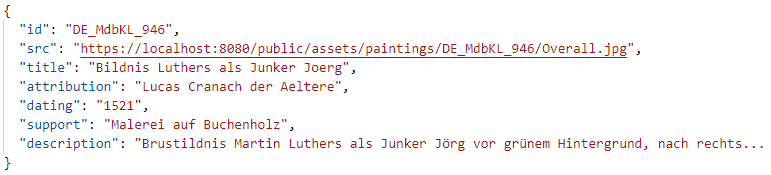
\includegraphics[scale=0.8]{img/coding/json-aufbau1.png}
          \caption{JSON-Struktur eines Gemäldes.}
          \label{fig:json-aufbau1}
        \end{figure}
        Da JavaScript beim Auslesen einer JSON-Datei nicht wissen kann,
        um was für ein Objekttyp es sich handelt, wird zusätzlich ein
        Objekt in TypeScript angelegt, um innerhalb des Codes Typssicherheit
        und eine verbesserte Unterstützung der Code Completion innerhalb
        einer Entwicklungsumgebung gewährleisten 
        zu können (siehe Abb. \ref{fig:painting-type1}). \\
        \begin{figure}[h]
          \centering
          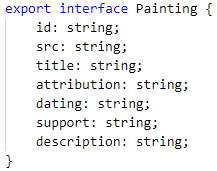
\includegraphics{img/coding/painting-type1.png}
          \caption{Gemälde-Interface in TypeScript.}
          \label{fig:painting-type1}
        \end{figure}
        Um ein Gemälde anhand einer JSON-Datei zu generieren,
        muss das Generieren vollständig auf JavaScript
        basieren, da das dynamische Auslesen aller Informationen
        nicht im HTML umgesetzt werden kann. Dafür wird eine 
        Komponente benötigt,
        welche die JSON-Datei ausließt und anhand der Daten ein Gemälde,
        dessen Informationen und Nahaufnahmen-Buttons generiert.
        Die Komponente \texttt{paintings-builder} wird der 
        \texttt{<a-scene>} hinzugefügt, da
        dies beim Erstellen der Szene ausgeführt werden soll. Die
        Komponente ist im Plural geschrieben, da die Option freigehalten
        werden soll, mehrere Gemälde generieren zu können.
        In ihrer \texttt{init}-Methode wird zuerst die JSON-Datei
        ausgelesen und bei Erfolg \texttt{createPainting(...)}
        ausgeführt (siehe Abb. \ref{fig:paintings-builder1}).
        Diese Methode bekommt ein Objekt des Typs \texttt{Painting}
        (Typdefinition siehe Abb. \ref{fig:painting-type1}). Zum aktuellen
        Zeitpunkt befindet sich in der JSON-Datei die Informationen
        zu nur einem Gemälde. Der Code ist jedoch so entwickelt wurden,
        dass er ohne viel Mehraufwand mehrere Gemälde entgegennehmen kann.
        \begin{figure}
          \centering
          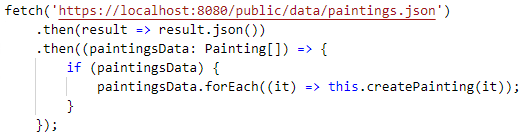
\includegraphics{img/coding/paintings-builder1.png}
          \caption{Abrufen der Daten innerhalb der \texttt{paintings.json}.}
          \label{fig:paintings-builder1}
        \end{figure}
        Innerhalb der \texttt{createPainting}-Methode wird das Gemälde
        , die Informationen und die Standing Area erzeugt. Bei der Standing
        Area handelt es sich um das selbe HTML, nur wurde dies in das
        JavaScript übersetzt. Da jedes Gemälde eine Standing Area benötigt,
        wird diese immer mit einem Gemälde mitgeneriert. Für das Verständnis
        der Umsetzung und um nicht den Rahmen zu sprengen, wird nicht 
        vollständig auf die \texttt{paintings-builder}-Komponente 
        eingegangen. \\
        Die relevantesten Codestellen innerhalb der 
        \texttt{paintings-builder} sind die, welche das Gemälde und
        die Informationen dazu generiert (siehe Abb. \ref{fig:paintings-builder2}).
        \begin{figure}
          \centering
          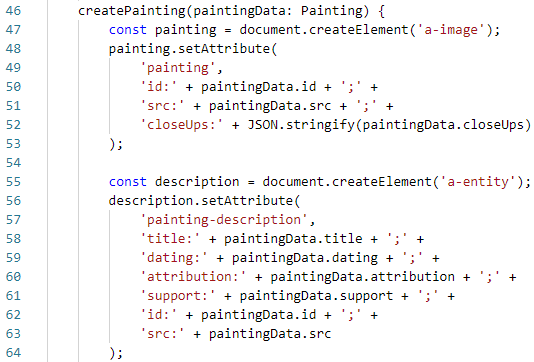
\includegraphics{img/coding/paintings-builder2.png}
          \caption{Codeabschnitt für die Generierung des Gemäldes und dessen Informationen.}
          \label{fig:paintings-builder2}
        \end{figure}
        Im Gegensatz zum vorherigen HTML, bekommen die Entitäten ihre Daten
        in ihre zugehörigen Komponenten hineingegeben. Das \text{<a-image>}
        -Tag bekommt nun eine Komponente namens \texttt{painting} und die 
        Informationen zum Gemälde werden weiterhin in einem \texttt{<a-entity>}
        -Tag gebündelt, jedoch bekommt dieses ebenfalls eine Komponente mit dem
        Namen \texttt{painting-description}. Beide Komponenten bekommen
        über ihr Schema die notwendigen Informationen, die sie benötigen
        (siehe Abb. \ref{fig:paintings-builder2}, Zeile 48-53 und Zeile 56-64).
        So wird kein HTML benötigt und die Daten können dynamisch ausgelesen
        und in die einzelnen Komponenten hineingegeben werden. \\
        Die \texttt{painting}-Komponente bekommt neben ihrer eigenen Gemälde-ID
        und deren Pfad zur Bilddatei noch die Informationen der einzelnen
        Nahaufnahmen, da diese innerhalb des Gemäldes generiert werden müssen.
        In der \texttt{init}-Methode dieser Komponente wird die 
        \texttt{createDetailPoints}-Methode aufgerufen 
        (siehe Abb. \ref{fig:painting1}).
        \begin{figure}
          \centering
          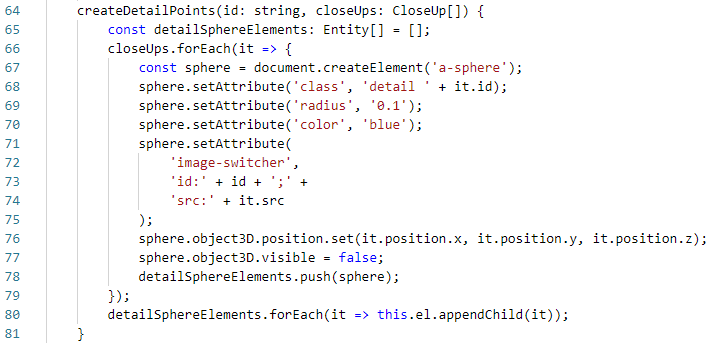
\includegraphics{img/coding/painting1.png}
          \caption{\texttt{createDetailPoints} innerhalb der \texttt{painting}-Komponente.}
          \label{fig:painting1}
        \end{figure}
        Diese nimmt folgende Argumente entgegen: \texttt{id: string} und
        \texttt{closeUps: CloseUp[]}. Die \texttt{id} des Gemäldes wird
        innerhalb der \texttt{image-switcher} Komponente benötigt. Die
        Informationen der Nahaufnahmen sind in dem Parameter 
        \texttt{closeUps} gespeichert. Dieses Objekt beinhaltet neben
        der \texttt{id} und \texttt{src} auch die Positionen der Punkte
        relativ zum Gemälde. In der \texttt{image-switcher}-Komponente
        wird der \texttt{click}-EventListener registriert, welcher bei
        einem Klick das Gemälde mit einer Nahaufnahme ersetzt und die 
        aktivierten Punkte ausblendet. Durch
        \texttt{visible = false} werden die Punkte initital unsichtbar gestellt
        (siehe Abb. \ref{fig:painting1}, Zeile 77). \\
        Die \texttt{painting-description}-Komponente aus Abbildung 
        \ref{fig:paintings-builder2} hat sich nicht stark
        zu seiner HTML-Version verändert. Er generiert zusätzlich noch
        eine \texttt{<a-box>}, welche den Button darstellen soll. Dieser
        Button erhält eine Komponente namens \texttt{detail-button}, welche
        bei Klicken das Anzeigen der möglichen Nahaufnahme-Punkten
        ermöglicht. Dabei erhält der Button den Schriftzug \glqq Zurück\grqq{}, 
        um von einer Nahaufnahme wieder zurück zum Gemälde umzuschalten. \\
        Der erste Prototyp ist somit fertig und zeigt ein Gemälde mit 
        Informationen an und einen Button, um die Details einzublenden
        (siehe Abb. \ref{fig:paintings-builder3}).
        \begin{figure}
          \centering
          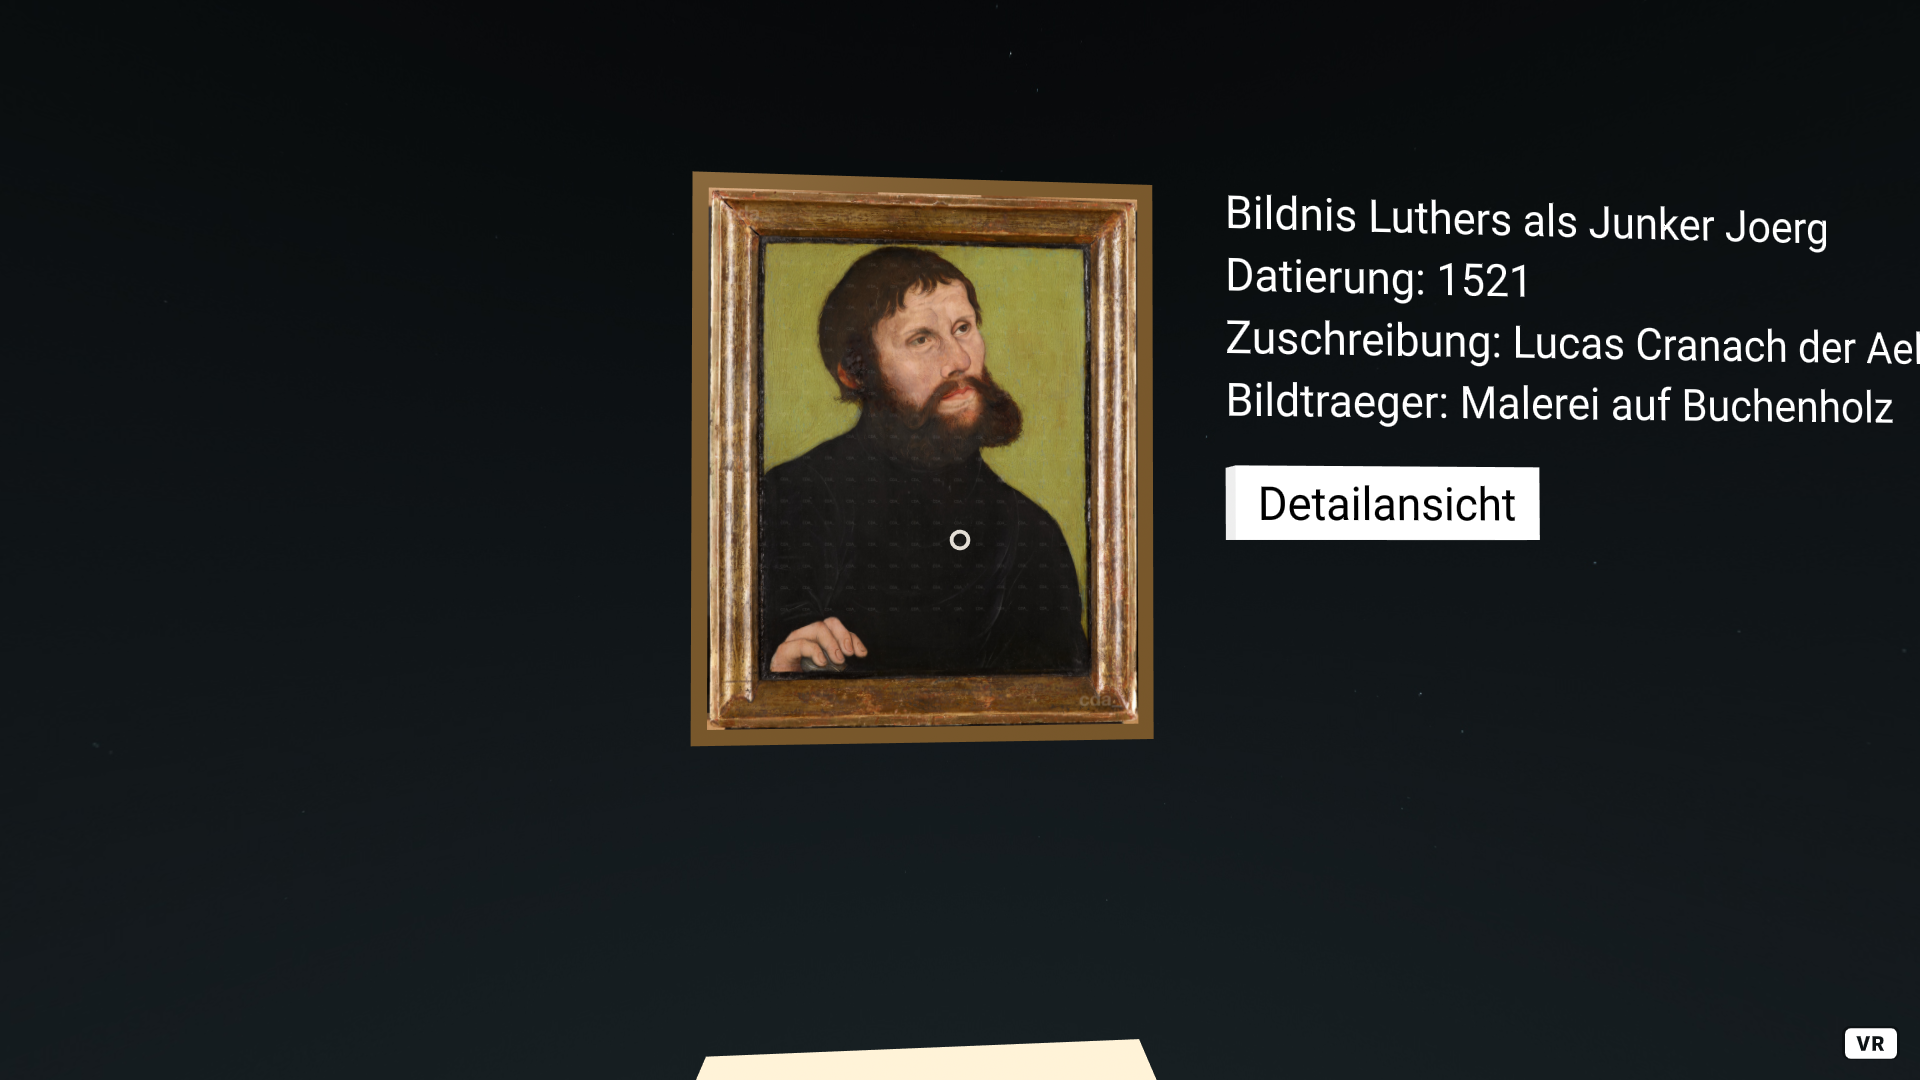
\includegraphics[scale=0.3]{img/coding/paintings-builder3.png}
          \caption{Ansicht des ersten fertigen Prototypen.}
          \label{fig:paintings-builder3}
        \end{figure}
        Klickt der Benutzer auf den Button \glqq Detailansicht\grqq{},
        erscheinen blaue Punkte auf dem Gemälde.
        (siehe Abb. \ref{fig:paintings-builder4}).
        \begin{figure}
          \centering
          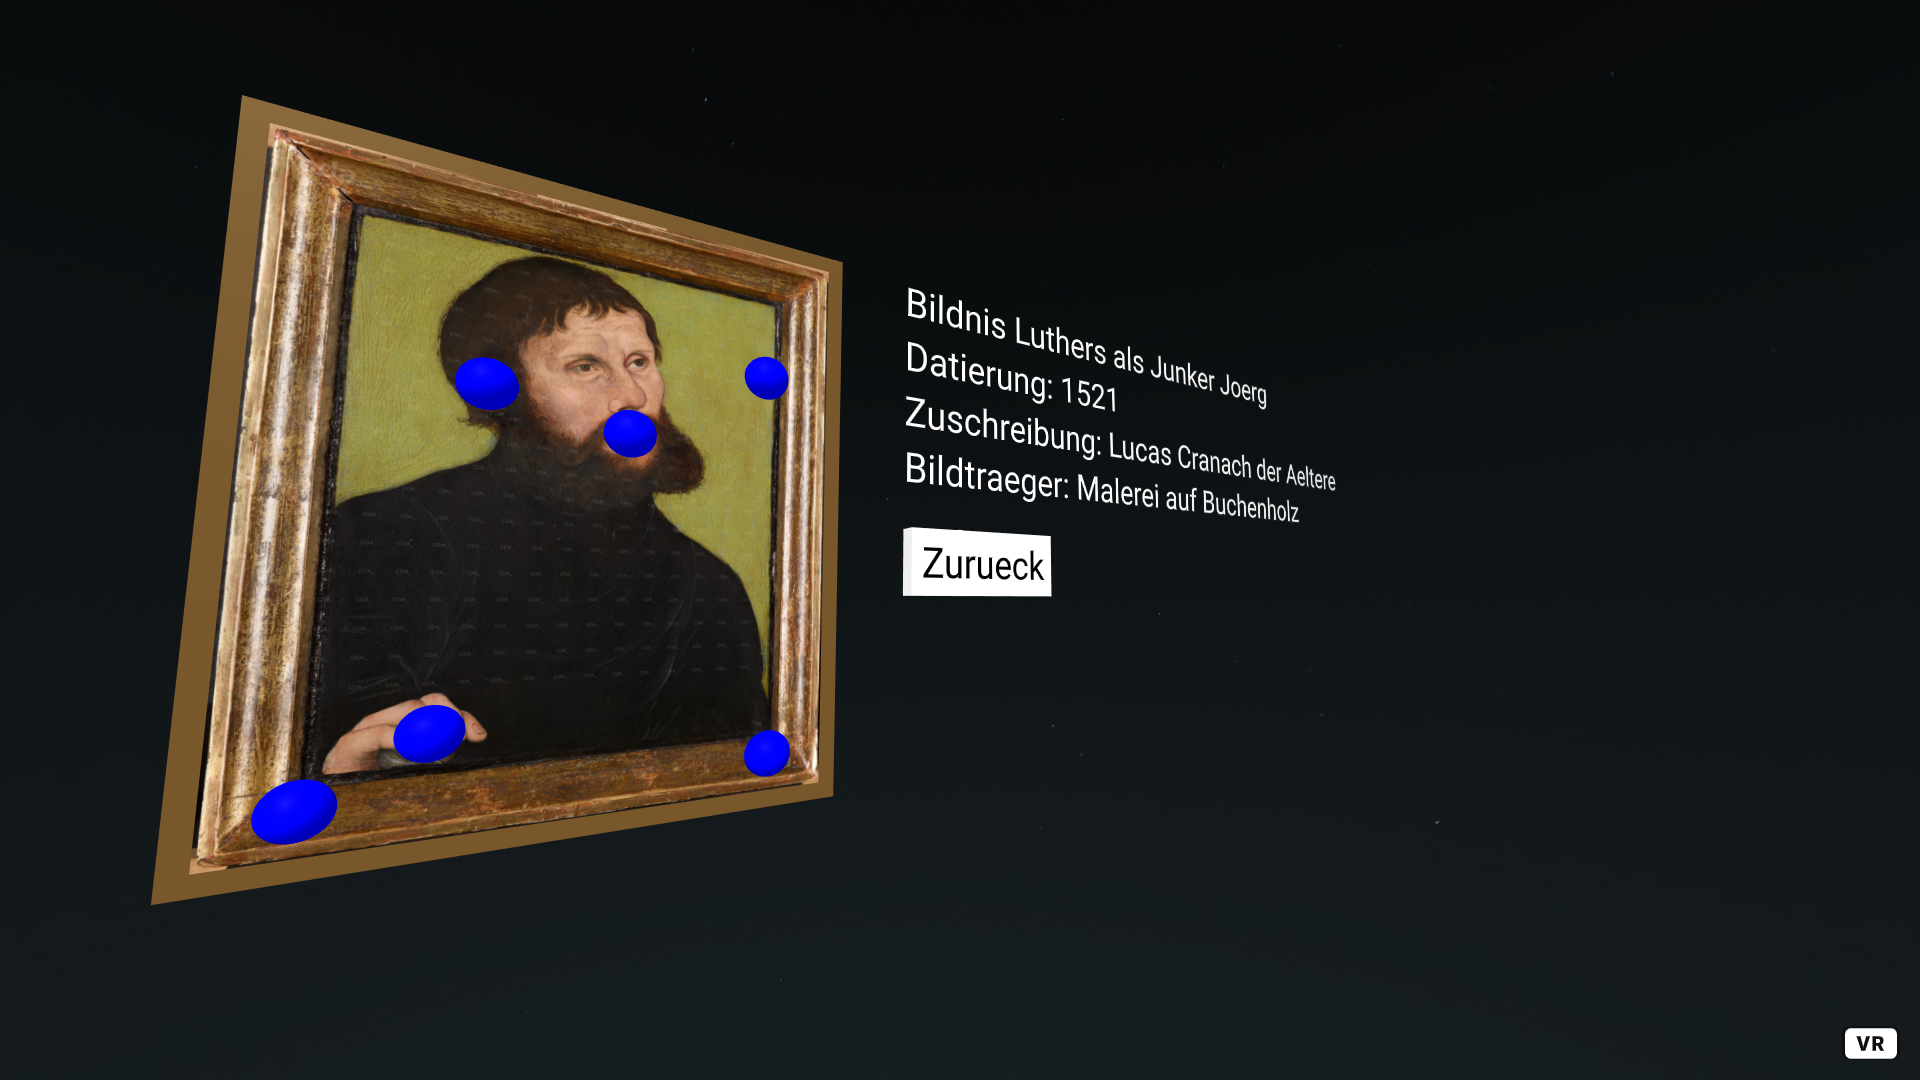
\includegraphics[scale=0.3]{img/coding/paintings-builder4.png}
          \caption{Detailpunkte auf dem Gemälde nach einem Klick auf den \glqq Detailansicht\grqq{}-Button.}
          \label{fig:paintings-builder4}
        \end{figure}
        Zu diesen markierten Stellen existieren Nahaufnahmen von dem Gemälde.
        Durch einen weiteren Klick auf einer der Punkte, wird das
        aktuelle Gemälde durch eine Nahaufnahme ersetzt
        (siehe Abb. \ref{fig:paintings-builder5}).
        \begin{figure}
          \centering
          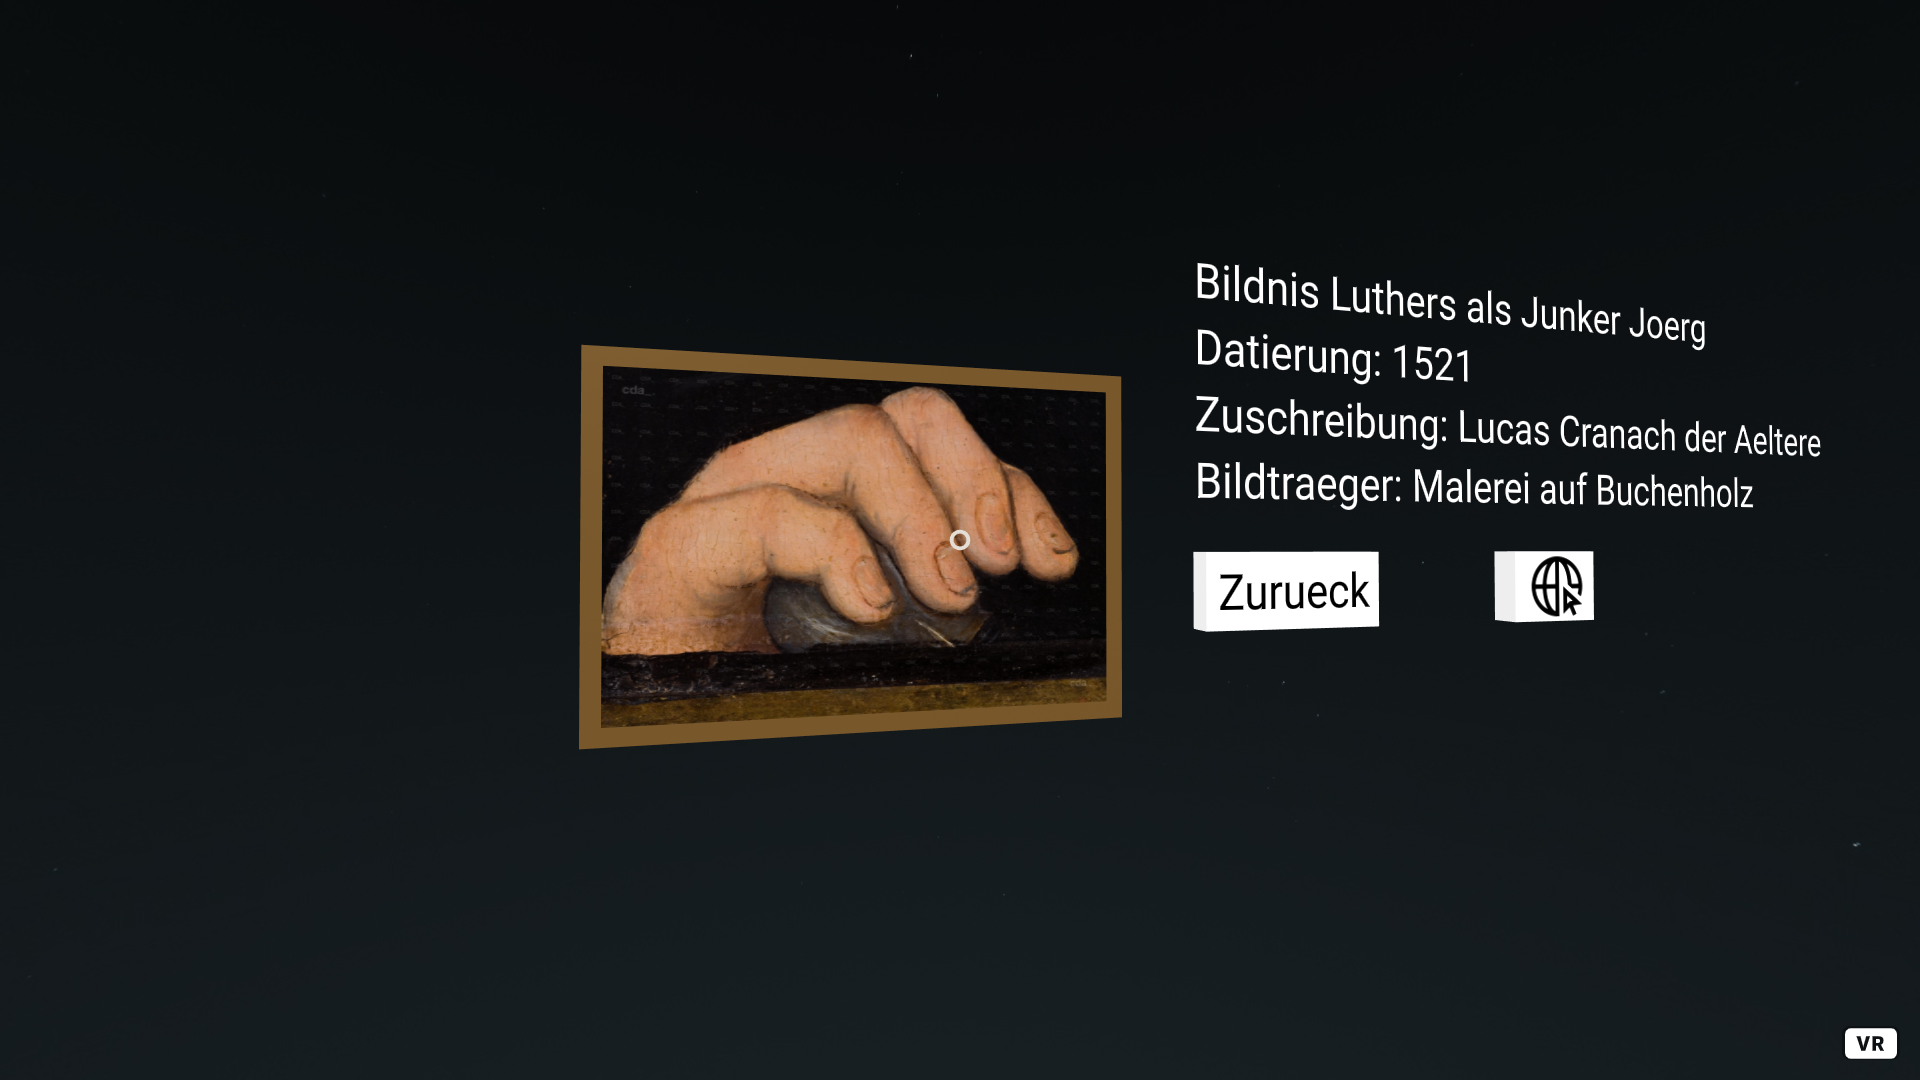
\includegraphics[scale=0.3]{img/coding/paintings-builder5.png}
          \caption{Eine Nahaufnahme des Gemäldes mit der ID \texttt{DE\_MdbKL\_946}.}
          \label{fig:paintings-builder5}
        \end{figure}
        Der erste technische Prototyp soll das Fundament der weiteren 
        Prototypen darstellen. Durch das komponentenbasierte System von
        A-Frame, lässt sich diese Art der Darstellung in andere Szenen
        und in einem anderen Kontext wiederverwenden.
      \subsubsection{Lucas Cranachs Werkstatt}
      Lucas Cranach d. Ä. entwarf vieler seiner Gemälde in seiner
      eigenen Werkstatt. Ähnlich wie das Deutsche Auswandererhaus soll
      bei diesem Prototyp der Benutzer in ein Szenario aus der Vergangenheit
      versetzt werden, um das Erlebnis immersiver zu gestalten. 
      Da Archivalien von Lucas Cranach d. Ä. zur 
      Verfügung stehen, wird ein Gemälde und 
      Dokumente aus dem selben Jahr genommen, um den Benutzer in einen
      Tag von Lucas Cranac d. Ä. zu versetzen. Die Schrift der Archivalien
      sind für den Benutzer unleserlich. Durch einen Klick
      auf einen Button soll die Beschreibung aus dem Cranach
      Digital Archive zu diesen Dokumenten vorgetragen werden. Das soll
      dem Benutzer das Gefühl geben, zu wissen, was bei Lucas Cranach d. Ä.
      an diesem Tag vorgegangen ist. \\
      Dieser Prototyp wird qualitativ nicht an eine hochwertige Produktion
      gelangen, wird aber zeigen, wie durch A-Frame solche Konzepte
      umgesetzt werden können. \\
      Um eine Werkstatt als Szene in A-Frame umzusetzen, werden 3D-Modelle
      benötigt. Nach einer kurzen Recherche bei Google haben sich
      Poly von Google\footnote{Poly von Google | \url{https://poly.google.com/} (18.11.2020)}
      und Sketchfab\footnote{Sketchfab | \url{https://sketchfab.com/} (18.11.2020)}
      als Plattformen für kostenfreie 3D-Modelle hervorgehoben. \\
      A-Frame bietet die Möglichkeit, ganze 3D-Modelle ebenfalls über ein
      HTML-Tag einzubinden. Dabei erlaubt das Framework das Einbinden von
      mehreren Datentypen, wie zum Beispiel glTF oder OBJ. In diesem Projekt
      wurde sich für glTF entschieden, da dies eine royalty-free Sepzifikation
      für 3D-Modelle, leichtgewichtig und interoperabel ist\footnote{glTF Overview | \url{https://www.khronos.org/gltf/} (18.11.2020)}.
      Sketchfab wie auch Poly bieten glTF als Dateiformat an. \\
      Das Einbinden eines glTF-Modells erfolgt über das A-Frame-Tag 
      \texttt{\textbf{<a-gltf-model>}}. Das Modell lässt sich über das Attribut
      \texttt{src} einbinden. Wie auch bei Bildern, kann der Pfad oder die ID
      aus dem \texttt{a-assets}-Tag genommen werden. Wird das 3D-Modell über
      \texttt{a-assets} eingebunden, muss dieses als \texttt{<a-asset-item>}
      hinzugefügt werden. Die Abbildung \ref{fig:gltf1} zeigt wie ein glTF-Modell 
      eingefügt werden kann.
      \begin{figure}
        \centering
        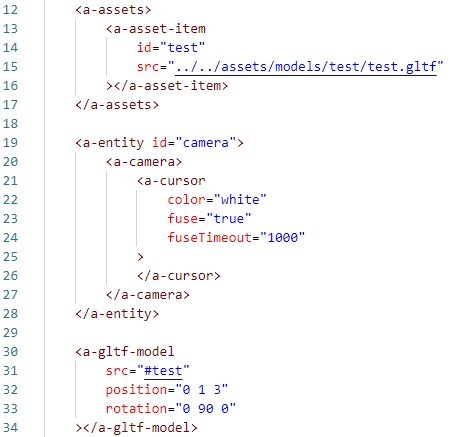
\includegraphics{img/coding/gltf1.png}
        \caption{Einbinden eines glTF-Modells in A-Frame über \texttt{<a-assets>}.}
        \label{fig:gltf1}
      \end{figure}
      Komponenten wie \texttt{painting}, \texttt{painting-description} und 
      \texttt{standing-area} können in diesem Prototypen wiederverwendet
      werden. Der einzige Mehraufwand entsteht durch die Modellierung
      der Werkstatt. Da fertige und kostenfrei Modelle aus dem Internet
      benutzt werden, entfällt dieser Aufwand ebenfalls. Die Werkstatt
      kann mittels A-Frame-Editor, welcher mit \texttt{STRG + ALT + I}
      innerhalb der Webanwendung aufgerufen werden kann. \\
      Die Werkstatt besteht aus zwei Teilen. Zum einen der Bereich des
      Gemäldes 
      (siehe Abb.)
      und zum anderen der Bereich der Dokumente
      (siehe Abb.).
      
  \section{Ergebnisse}
    \begin{itemize}
      \item Hier verwendet man beschriebene Methoden an
      \item Beschreiben, wie Untersuchung verlaufen ist
      \item Ergebnisse analysieren
    \end{itemize}
  \section{Diskussion und Fazit}
    \begin{itemize}
      \item Folgen und Ursache der Ergebnisse beschreiben
      \item Limitationen und Vorschläge für zukünftige Projekte darlegen
    \end{itemize}
    -
    \begin{itemize}
      \item Auf wichtigste Ergebnisse eingehen
      \item Geht auf Einleitung ein, da auf Forschungsfrage eingeht
      \item Füge keine neuen Informationen und Interpretationen
      \item Füge keine Beispiele und Zitate ein, bleibe bei den Fakten
      \item Dein Ergebnis ist immer wertvoll
      \item Ergebnisse deiner Forschung werden im Präsens geschrieben
    \end{itemize}
  \section{Anhang}
    \subsection{Quellenverzeichnis}
      \printbibliography
  
  \newpage
  \pagestyle{empty}
  \section*{Erklärung über die selbständige\\Abfassung der Arbeit}
    \addcontentsline{toc}{section}{Erklärung über die selbständige Abfassung der Arbeit}
    Ich versichere, die von mir vorgelegte Arbeit selbständig verfasst zu haben.
    Alle Stellen, die wörtlich oder sinngemäß aus veröffentlichten oder nicht veröffentlichten Arbeiten anderer entnommen sind,
    habe ich als entnommen kenntlich gemacht.\\ 
    Sämtliche Quellen und Hilfsmittel, die ich für die Arbeit benutzt habe, sind
    angegeben. Die Arbeit hat mit gleichem Inhalt bzw. in wesentlichen Teilen noch keiner anderen Prüfungsbehörde vorgelegen.\\\\
    \begin{tabular}{cp{7cm}}
      & \\ 
      & \\ \hline
      \small (Ort, Datum, Unterschrift) & \normalsize \\
    \end{tabular}
  
  \newpage

  % Unbeschriftetes Abschlussblatt (Leere Seite)
  \thispagestyle{empty}
  \section*{}  
          
\end{document}